\documentclass[a4paper,12pt]{report}
\usepackage{graphicx}
\usepackage{cancel}	%para cancelar expresiones en fórmulas
\usepackage{multicol}
\usepackage{multirow}
\usepackage{amsmath}
\usepackage{float}
\usepackage{url}
\usepackage{color}
\usepackage{tablefootnote}
\usepackage[12pt]{moresize}	%más tamaños de letra
\usepackage{bm}	%bold para math

\usepackage{titlesec}
%\titleformat{\chapter}[display]
%{\normalfont\bfseries}{}{12pt}{\Huge}	%quitar header de chapter

\usepackage{siunitx}	%support for units, numbers
\sisetup{output-decimal-marker={.}, separate-uncertainty}

\usepackage{hyperref}
\hypersetup{
	colorlinks=true,
	linkcolor=blue,
	citecolor=red,
	bookmarksopen=true,
	bookmarksopenlevel=1,
	urlcolor=blue
}

\usepackage{tikz}	%%TIKZ for drawings, shapes
\usetikzlibrary{positioning}
\tikzset{
	nodo/.style={
		rectangle,
		draw,
		black,
		thick,
		rounded corners,
		node distance=1.5cm,
		inner sep=0.3cm,
		font=\large
	}
}

%%% NOMBRES DE COSAS
\renewcommand{\abstractname}{Abstract}
\renewcommand{\figurename}{Figure}
\renewcommand{\tablename}{Table}
\renewcommand{\contentsname}{Table of Contents}
\renewcommand{\appendixname}{Appendix}
\renewcommand{\bibname}{References}
\renewcommand{\chaptername}{Part}

%%% COMANDOS COMUNES
\newcommand{\dif}{\text{d}}
\newcommand{\ddt}[1]{\frac{\dif #1}{\dif t}}
\newcommand{\der}[2]{\frac{\dif #1}{\dif #2}}
\newcommand{\mder}[3]{\frac{\dif^{#3}#1}{\dif #2^{#3}}}		%derivada múltiple
\newcommand{\norm}[1]{\left\| #1 \right\|}
\newcommand{\an}{($\alpha$,n) }
\newcommand{\Aliso}{\textsuperscript{27}Al }
\newcommand{\Piso}{\textsuperscript{30}P }
\newcommand{\Na}{\textsuperscript{22}Na }

%%%%%%%%%%%%%%%%%%%%%%%%%%%%%%%%%%%%%%%%%%%%%%%%%%%%%%%%%
\usepackage[a4paper]{geometry}
\geometry{top=2cm,bottom=2cm,left=1.8cm,right=1.8cm}
\usepackage{setspace}	%interlineado
\onehalfspace	%interlineado 1.5

\makeindex
%%%%%%%%%%%%%%%%%%%%%%%%%%%%%%%%%%%%%%%%%%%%%%%%%%%%%%%%%
\begin{document}
\begin{titlepage}
	\centering
	\Huge Inter-University Master's degree in Nuclear Physics\par
	\vspace*{3cm}
	\HUGE \textbf{Measurements of ($\bm{\alpha}$,n) reactions in CNA/HiSPANoS}\par	%TBD? más largo?
	\vspace{1cm}
	
\includegraphics[width=0.35\textwidth]{us.png}\\
	\vspace{1cm}
	\Large \textsc{Erik Cárdenas Mayoral}\par
	\vspace{2cm}
	Supervisors:\\
	Carlos Guerrero Sánchez\\
	María Begoña Fernández Martínez\par
	\vfill
	26/06/2023
\end{titlepage}

\begin{abstract}
English abstract.
\\
Abstract español.
\end{abstract}

\tableofcontents

\chapter{Introduction and motivation}
In \an nuclear reactions, an alpha particle ($^4_2\text{He}^{2+}$) hits a target nucleus ($^\text{A}_\text{Z}\text{X}$) and a neutron is ejected.
Generally, in the laboratory frame of reference, the $\alpha$ is fast-moving and the target is stationary.
The produced neutron will also be fast, and the resulting nucleus ($^{\text{A}+3}_{\text{Z}+2}\text{Y}$) will be of a new element and have a small recoil.

\begin{figure}[H]
	\centering
	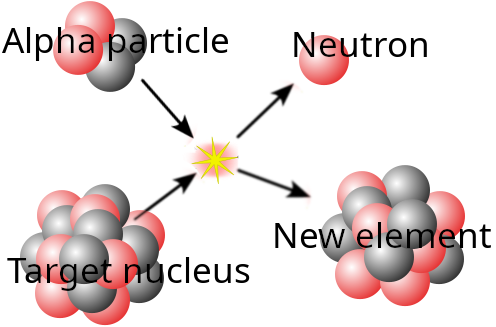
\includegraphics[width=0.4\textwidth]{anreaction.png}
	\caption{Illustration of an \an reaction.}
	\label{anreaction}
\end{figure}

Underground experiments trying to detect dark matter WIMPs or other rare events have to deal with neutron backgrounds that are hard to distinguish from the desired particles.
The main contribution to this background comes from \an reactions, produced by alphas coming from the radioactive decay of elements in the ground.\cite{neutron_in_an}.	%TBD:citas más relevantes, ésta lo da por sabido

A good knowledge of the cross-section and neutron spectra of these reactions is thus useful to differentiate between background counts and rare events.
\\

·Actual state of \an measurements.\\

·The objective of the measurements at CNA are to check the viability for carrying out more \an measurements.\\


\chapter{Experimental setup}
The source of alphas for the experiment is the \qty{3}{\mega\volt} tandem accelerator at CNA, which fires alphas at a \Aliso target.
Detectors used are both organic and inorganic scintillators.

\begin{figure}[H]
	\centering
	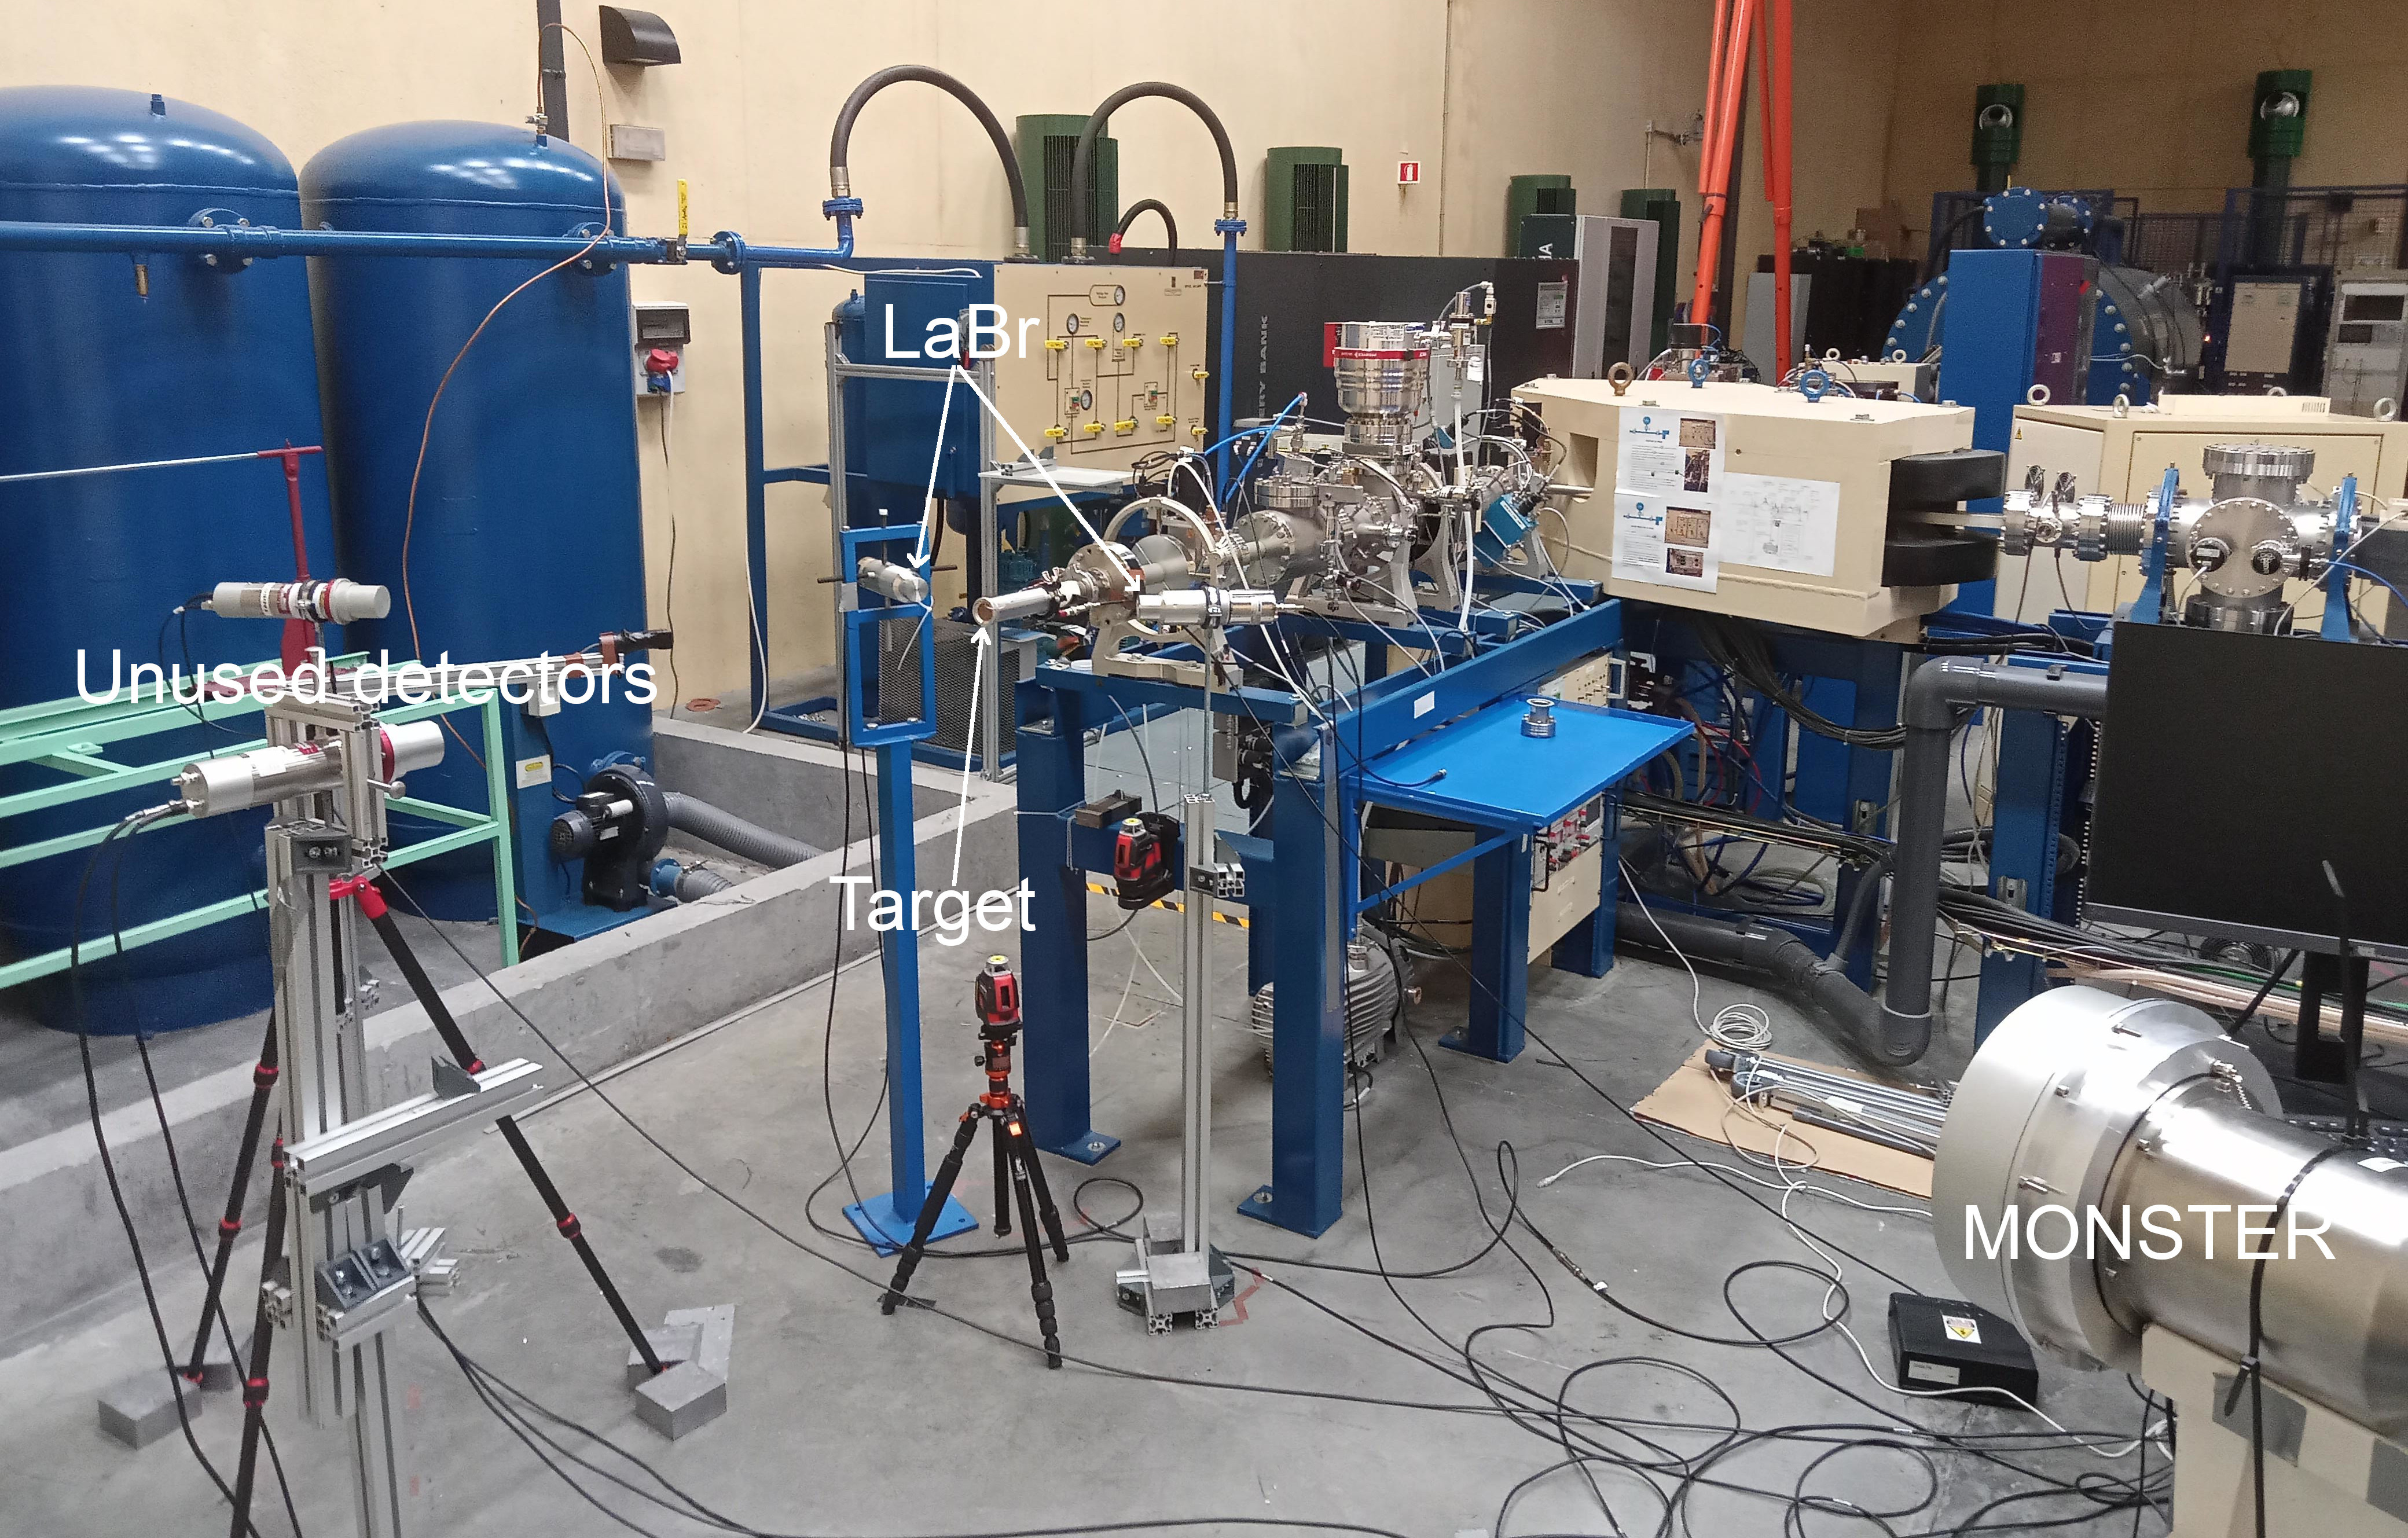
\includegraphics[width=0.80\textwidth]{overview_photo.jpg}
	\caption{Overview picture of the experimental setup.
	Detectors and the target are labeled.}
	\label{overview_photo}
\end{figure}

\section{Tandem 3MV accelerator}
A tandem is a type of linear particle accelerator whose main characteristic is that particles are accelerated twice by the same terminal voltage.
Particles are injected with negative charge from a source situated outside the tank, and accelerated toward the terminal.

Once the negatively charged particles arrive a the terminal, their electrons are removed by a gas, called the \textit{stripper}.
Now with a positive charge, they are accelerated the rest of the way by the same voltage.
\\

In the case of alpha particles, they are injected with charge -1, and then stripped of all electrons, to charge +2.
Given that the maximum voltage of the CNA tandem accelerator is \qty{3}{\mega\volt}, alphas can be accelerated to a maximum of $3\cdot\left(1+2\right) = \qty{9}{\mega\eV}$.	%TBD:añadir injection energy
\\

\subsection{Pulsed beam mode}
For most applications, the accelerator generates a continuous stream of particles.
But it can also be operated in a \textit{pulsed beam} manner, where particles are emitted in groups, or \textit{pulses}.

Ideally, those pulses are instantaneous: all particles arrive at exactly the same time.
In reality, they are approximated by a gaussian distribution, with a certain width in the order of a few nanoseconds.	%TBD: anchura exacta?
\\

To achieve pulsed operations, the accelerator uses two devices: the \textit{chopper} and the \textit{buncher}.
The \textit{chopper} generates an electric field that deflects all particles coming from the accelerator.
With a X frequency, it disengages the field and lets particles pass for X time.	%TBD: poner valores

After the chopper, the \textit{buncher} uses further electric fields to slow down the faster particles and accelerates the slower ones, making the pulse narrower in time (X) and gaussian shaped.	%TBD:poner valor
\\

\subsection{Difficulties with accelerating alpha particles}	%TBD:replace with bold symbol
Although it is used in this experiment to accelerate alphas, the CNA Tandem accelerator was not designed with them in mind.
Rather, it was designed to accelerate deuterons, which have the same mass-to-charge ratio.
This means that, while alphas can be also be accelerated, some problems arise when generating pulses.

The reason is that the electric fields used by the buncher to shape pulses are not strong enough.
This produces both wider and asymmetric pulses than with deuterons, as well as smaller overall currents; especially at higher energies (figure \ref{uneven_gflash}).
\\

\subsection{Neutron line}
·Explain the different parts of the neutron line. Photos.\\

\section{Target}
The target is a sheet of \qty{95}{\percent} purity \Aliso.	%TBD:confirmar porcentaje
This metal was chosen because it is relatively well known compared to others, with the best available measurements of \an reactions to compare to.
\\

Because the target is thick (more than a few micrometers), all of the alphas will be completely stopped by it.
This means that, for some of the \an reactions, the alpha particles will have lost part of their energy in the material.

Any measurements taken with a thick target are thus integrated measurements, for energies up to the one the alphas were accelerated to.
If we wanted to measure only \an reactions at a specific energy, we would have to use a very thin sheet of aluminium, so as to stop the alphas from being slowed down.
\\

It is important, in order to obtain quantitative results, to know how many alphas hit the target.
Because they are stripped of all their electrons, they have charge +2 when they arrive at the target.\footnote{Because the neutron line is aligned with the accelerator, using the \qty{90}{\degree} electromagnet to eliminate other charge states is not possible. Nontheless, the number of alpha particles with charge +1 is considered small enough as to be ignored.}
The target is not grounded, and so it charges up positively as alphas impact it.
By measuring the charge on the target, we can know how many alphas have hit it.

To do so, we connect the target via a copper wire to a \emph{charge integrator}, a device that emits a pulse and discharges the target each time it reaches \qty{0.1}{\nano\coulomb}, or approximately \num{3E8} alphas.
It is important that the target does not accumulate too much positive charge, as that could slow down or deflect incoming particles.

\begin{figure}[H]
	\centering
	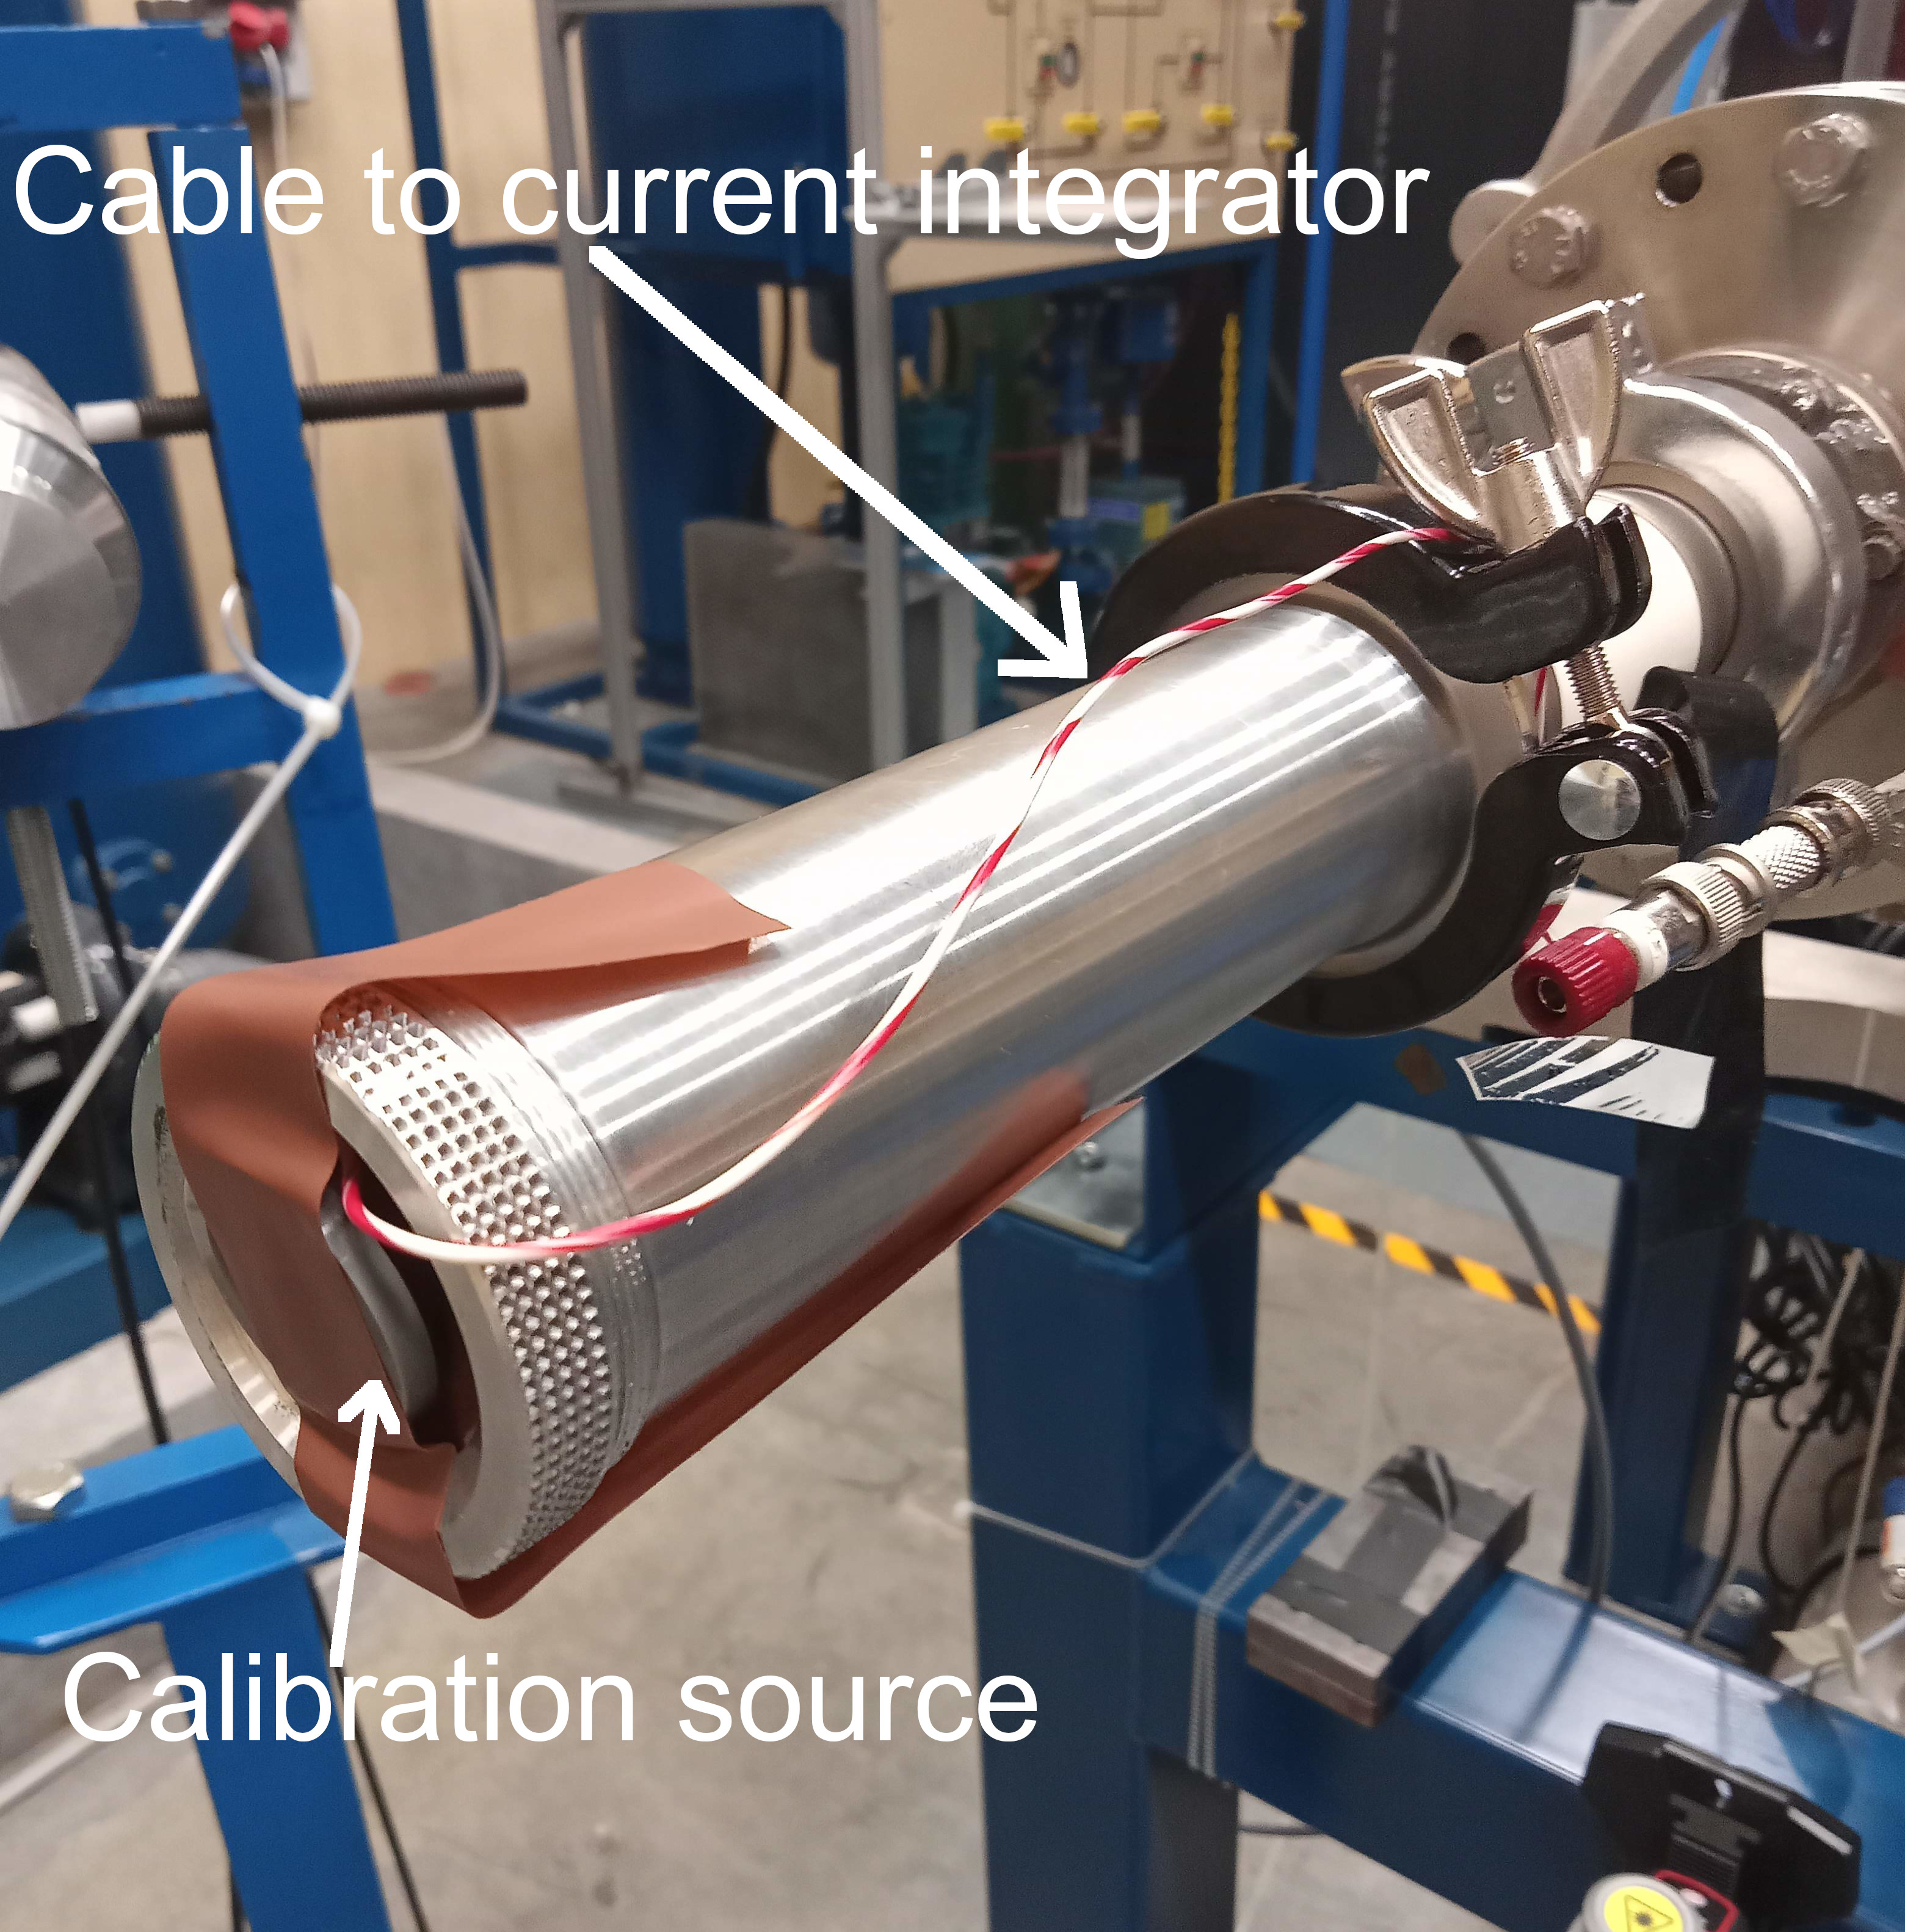
\includegraphics[width=0.5\textwidth]{target_with_calibration.jpg}
	\caption{Target at the end of the neutron line, with a calibration source taped for efficiency calibration measurements.}
	\label{target_photo}
\end{figure}

\section{Radiation detectors}
The thick target yield (number of \an reactions per number of incident alphas) will be measured by using gamma detectors, while the \an neutron spectra will be done via time of flight measurements with a neutron detector.
\\

·Drawing with distances and angles of all relevant detectors.\\

\begin{table}[H]	%Tabla con distancias y ángulos de detectores
\centering
\begin{tabular}[c]{>{\bfseries}l||c|c}
	Detector		&Distances\tablefootnote{Detectors were moved in order to get measurements at different distances.} (\unit{\cm})& Angle\\ \hline
	\textbf{MONSTER}	&\num{100}, \num{200}			&\qty{60}{\degree}	\\ \hline
	\textbf{LaBr1}		&\num{20}, \num{10}, \num{30}		&\qty{150}{\degree}	\\ \hline
	\textbf{LaBr2}		&\num{20}, \num{30}			&\qty{210}{\degree}	\\ \hline
\end{tabular}
\caption{Angles and distances of detectors.}
\label{distances_angles_table}
\end{table}

\subsection{LaBr}
To measure gammas, we use two LaBr\textsubscript{3} (lanthanum bromide) detectors, which we refer to as "LaBr1" and "LaBr2".
They are inorganic scitillators, meaning they produce light when hit by ionizing radiation.
This can be used to detect gamma rays by the following process:

When a gamma ray hits the material, it gives all of its energy via the photoelectric effect, or part of it through Compton scattering; to an electron in the medium.
This electron travels the scintillator, losing energy by exciting atoms.
When those excited states decay, they emit a \textit{scintillating} light, to which the material is transparent.

This \textit{scintillating} light is directed to a photocathode, where it emits electrons via the photoelectric effect.
These \textit{photo-electrons} are multiplied in a \textit{photomultiplier tube} (PMT), and finally turned into an electric pulse, which is registered as a detection.

Because proportionality is maintained in each of those conversions, we get a spectroscopic response, where more energetic gammas generate proportionately bigger pulses.
\\

To calculate the detectors' efficiency to \qty{511}{\keV} gammas, we use a \Na source that we stick on the target, at the end of the neutron line.
By fitting the resulting peak to a gaussian, we get the number of detected photons per second.
We then divide by the total number of emmited photons (given the source's activity) to get the efficiency.
\begin{equation}
	\text{detector efficiency} = \frac{\text{counts per second}}{\text{total source emissions}}
\end{equation}

\begin{figure}[H]
	\centering
	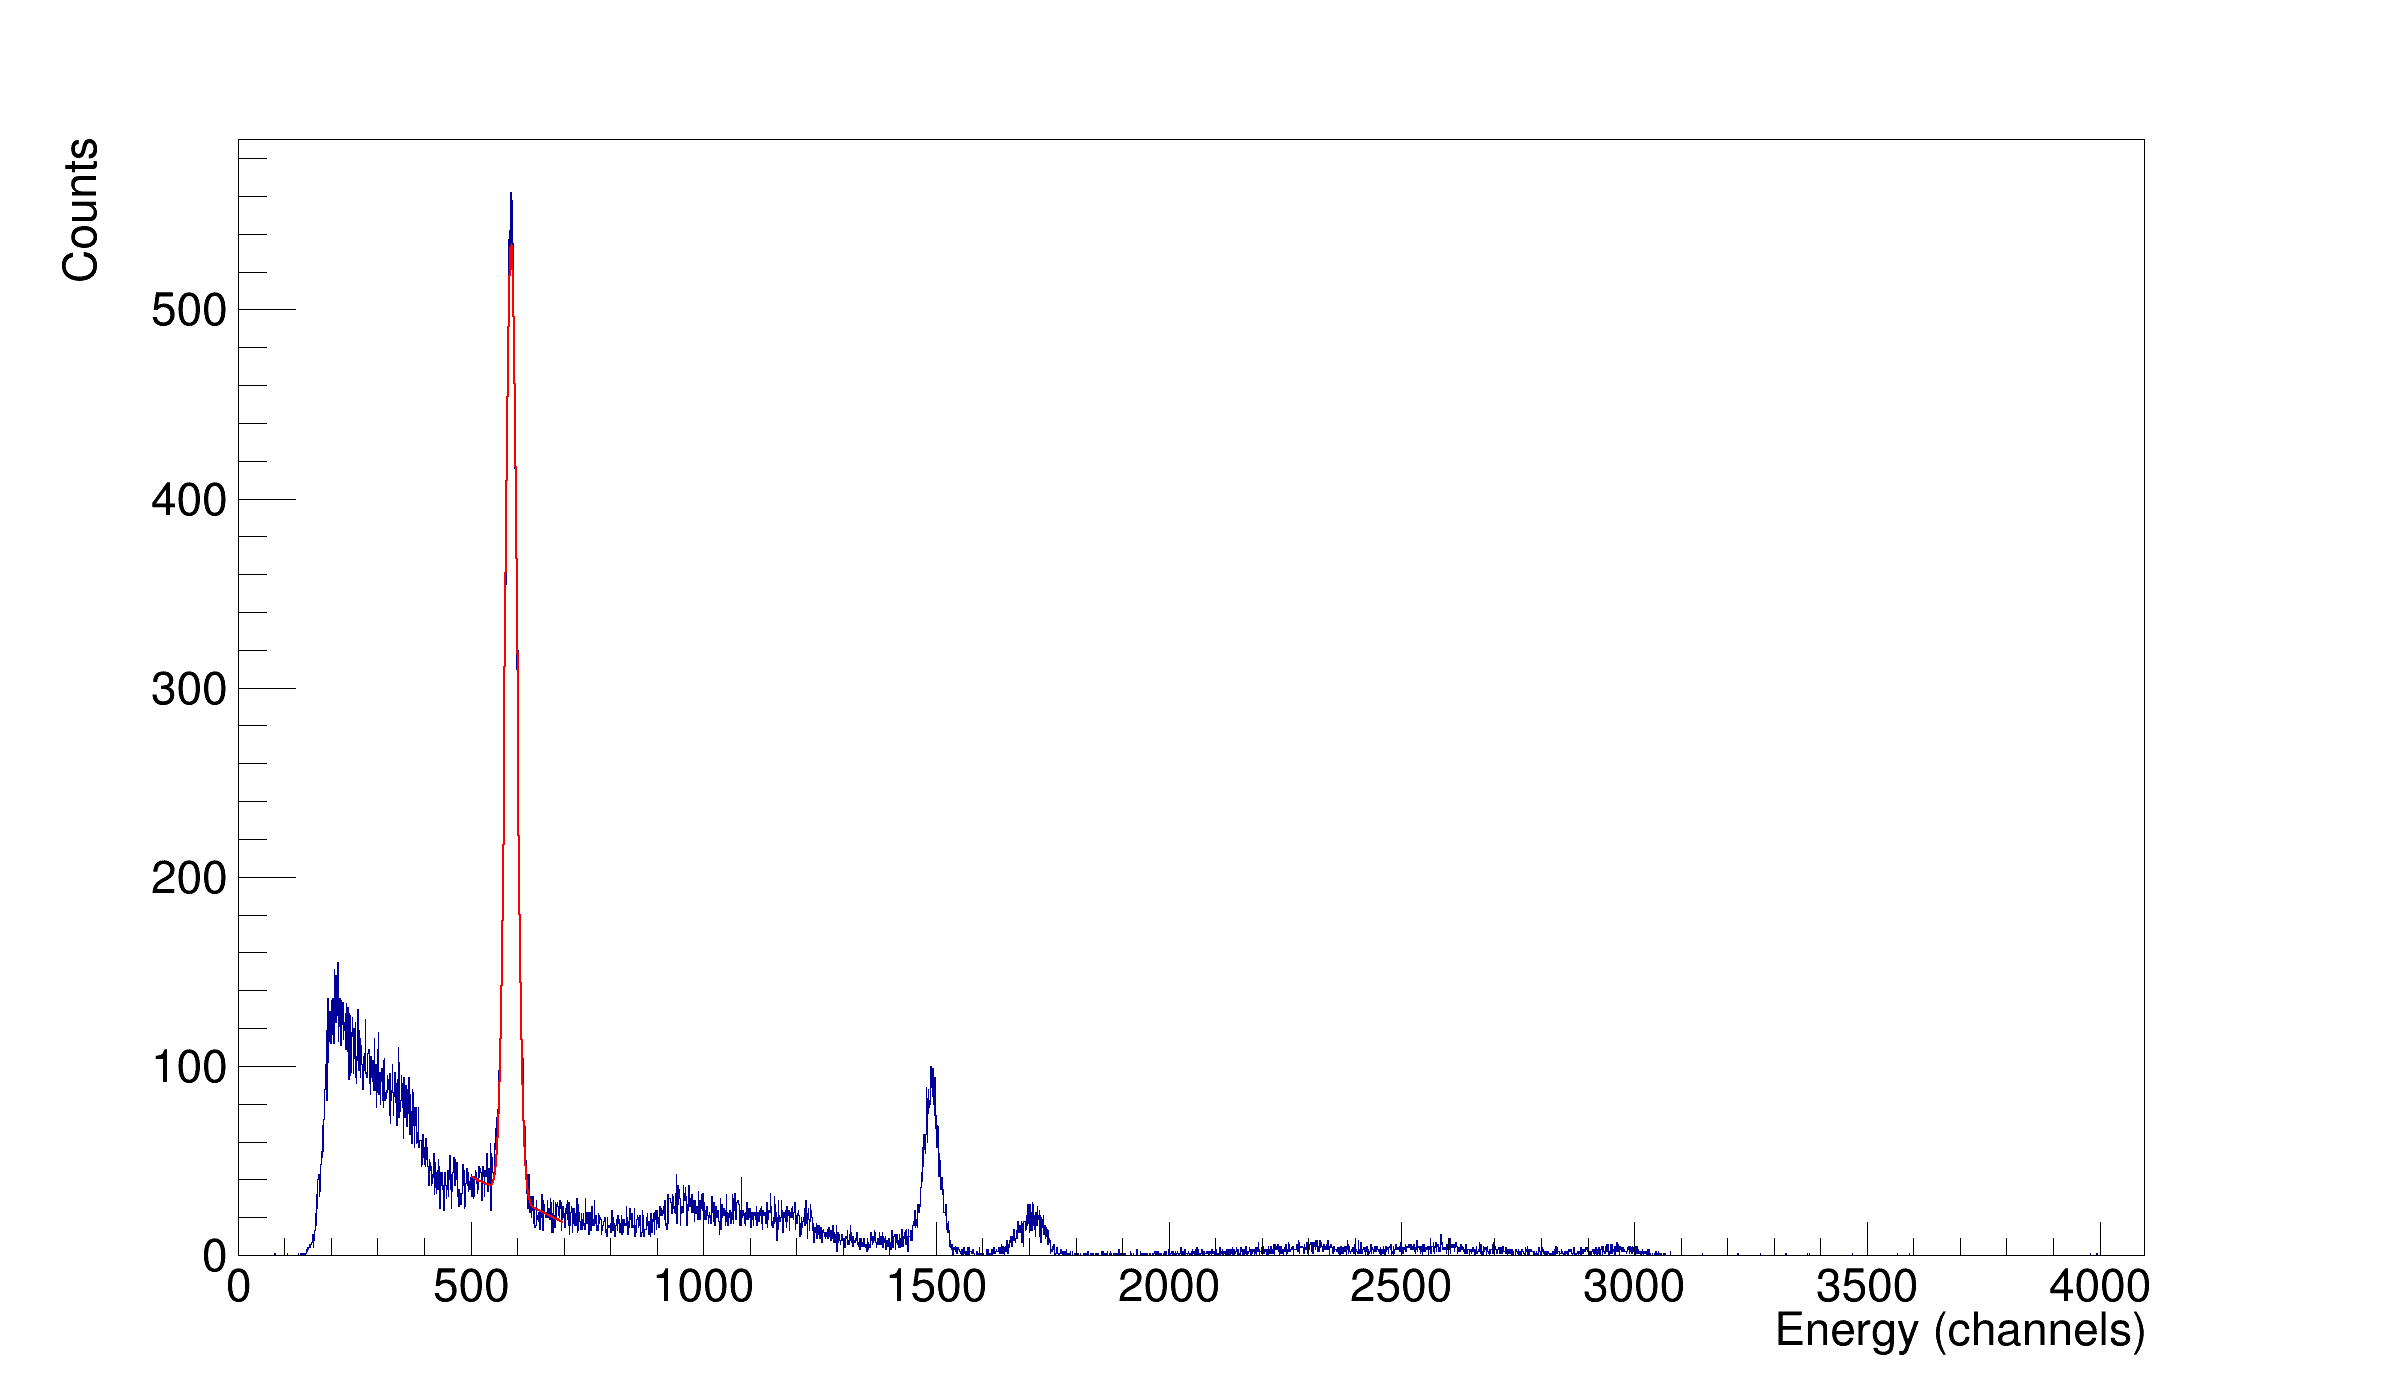
\includegraphics[width=0.80\textwidth]{labr_na22_calibration.png}
	\caption{LaBr1 response to \Na calibration source. In red is the fitting of the \qty{511}{\keV} peak to a gaussian plus a linear background.}
	\label{labr_na22_calibration}
\end{figure}

\begin{figure}[H]
	\centering
	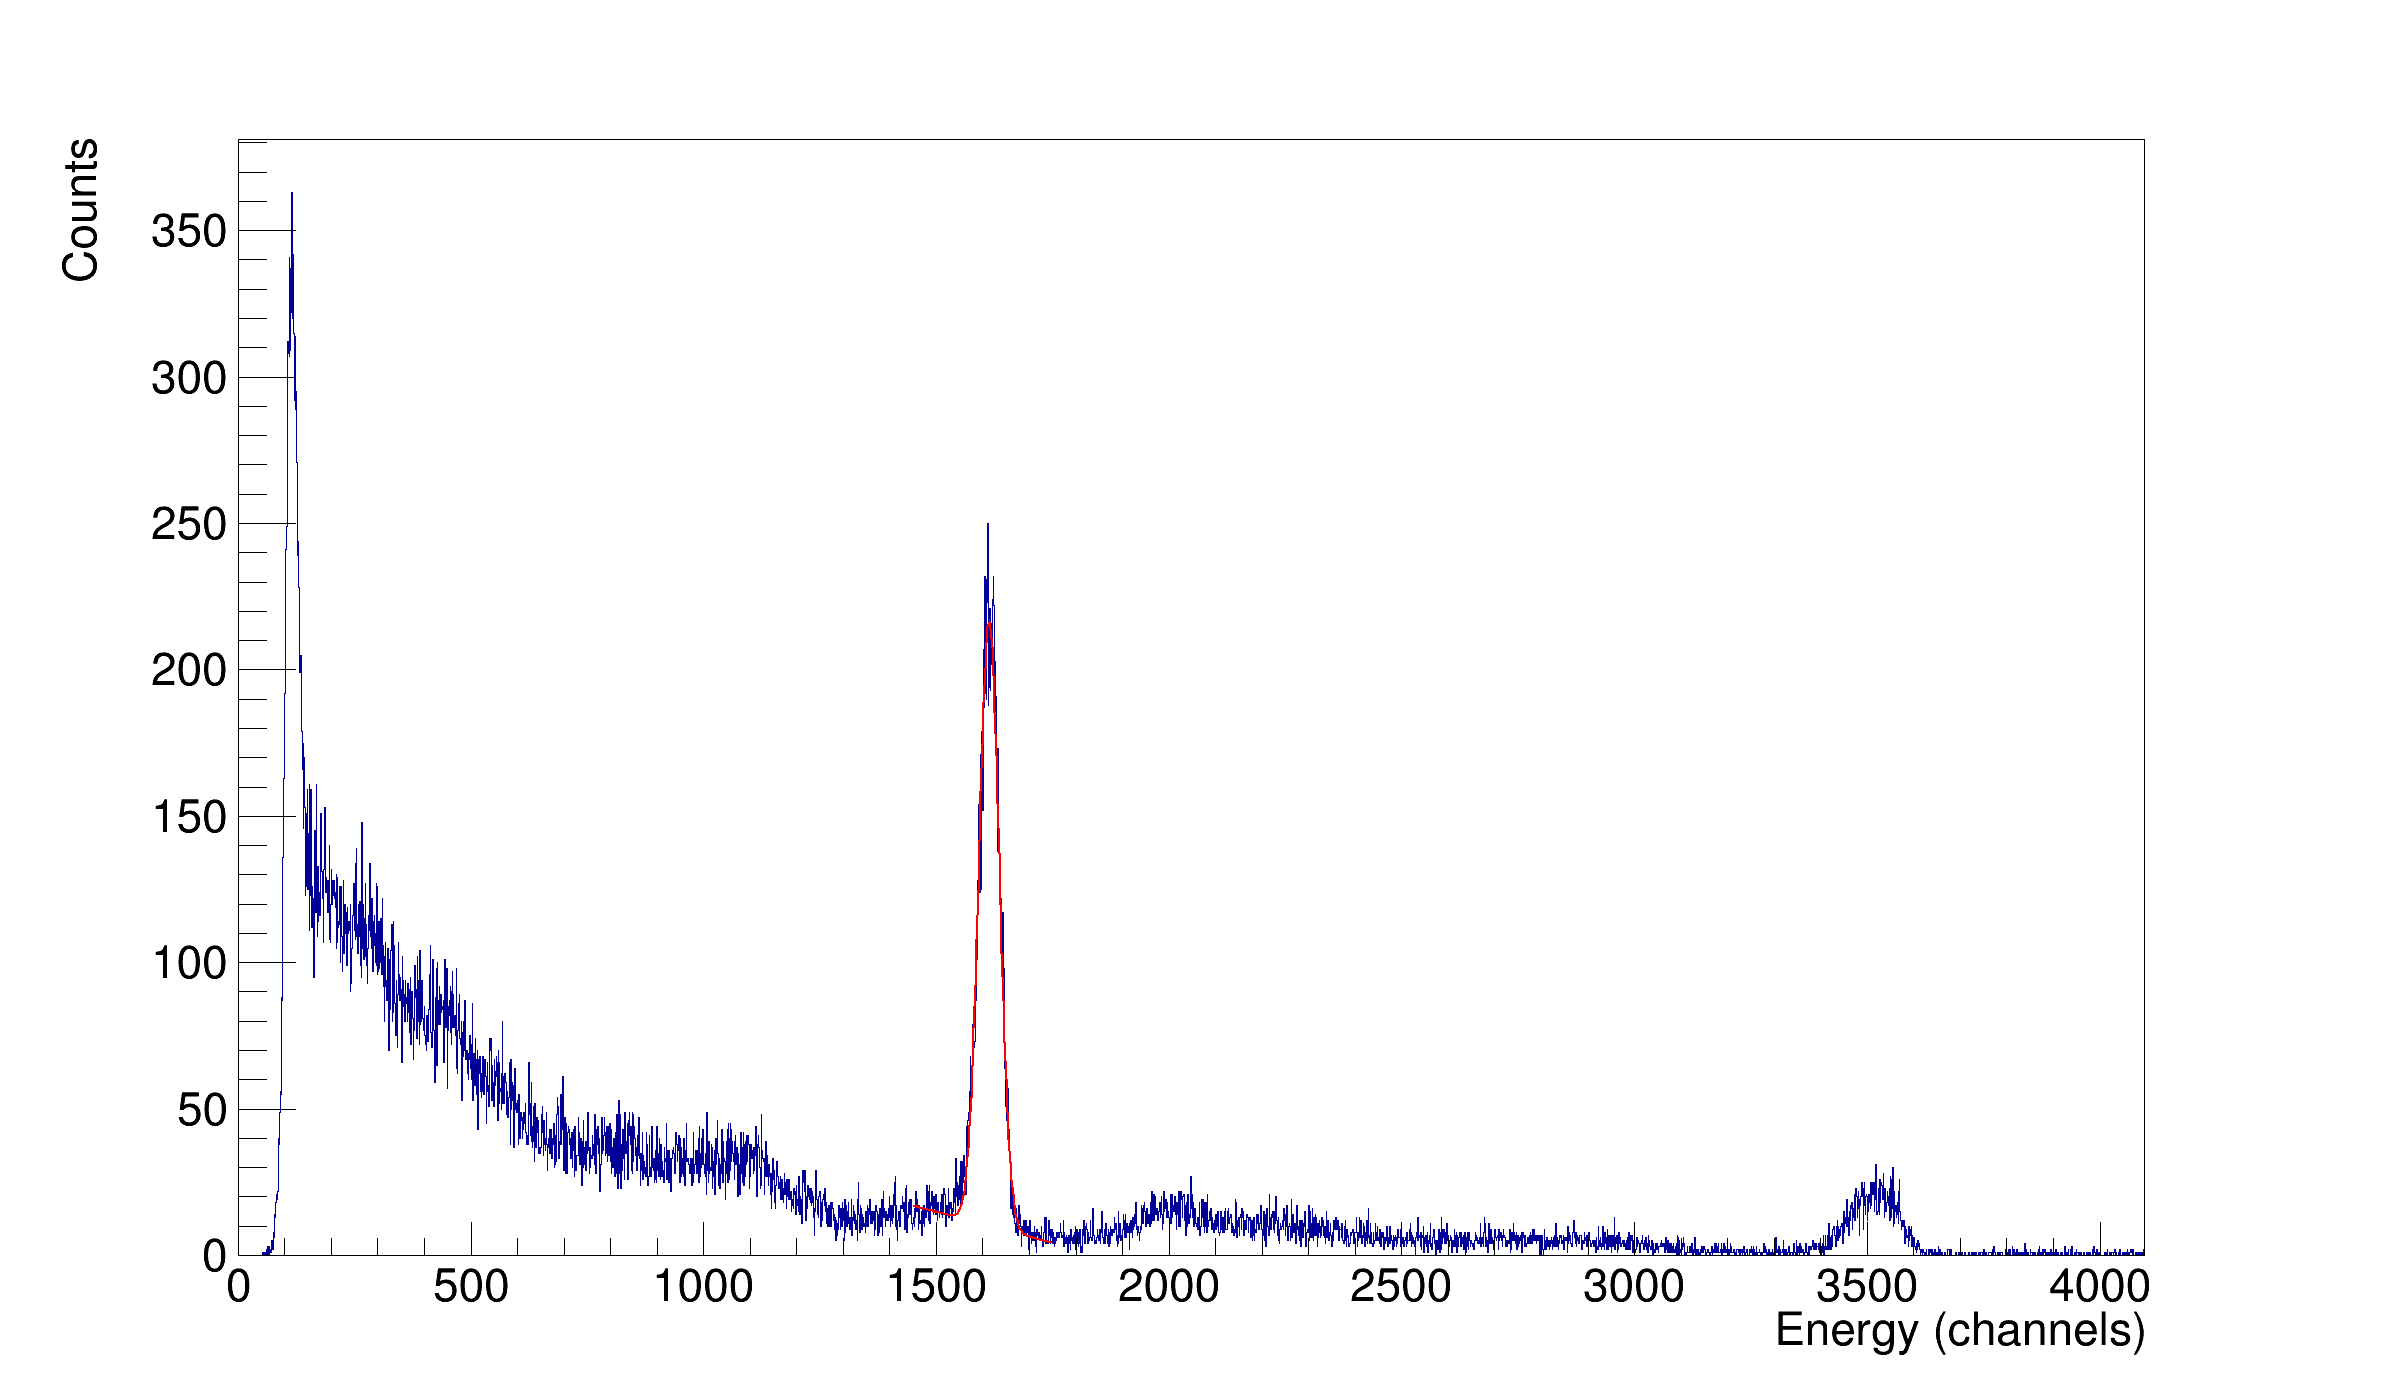
\includegraphics[width=0.80\textwidth]{labr_cs137_calibration.png}
	\caption{LaBr1 response to \textsuperscript{137}Cs calibration source.}
	\label{labr_cs137_calibration}
\end{figure}

\begin{figure}[H]
	\centering
	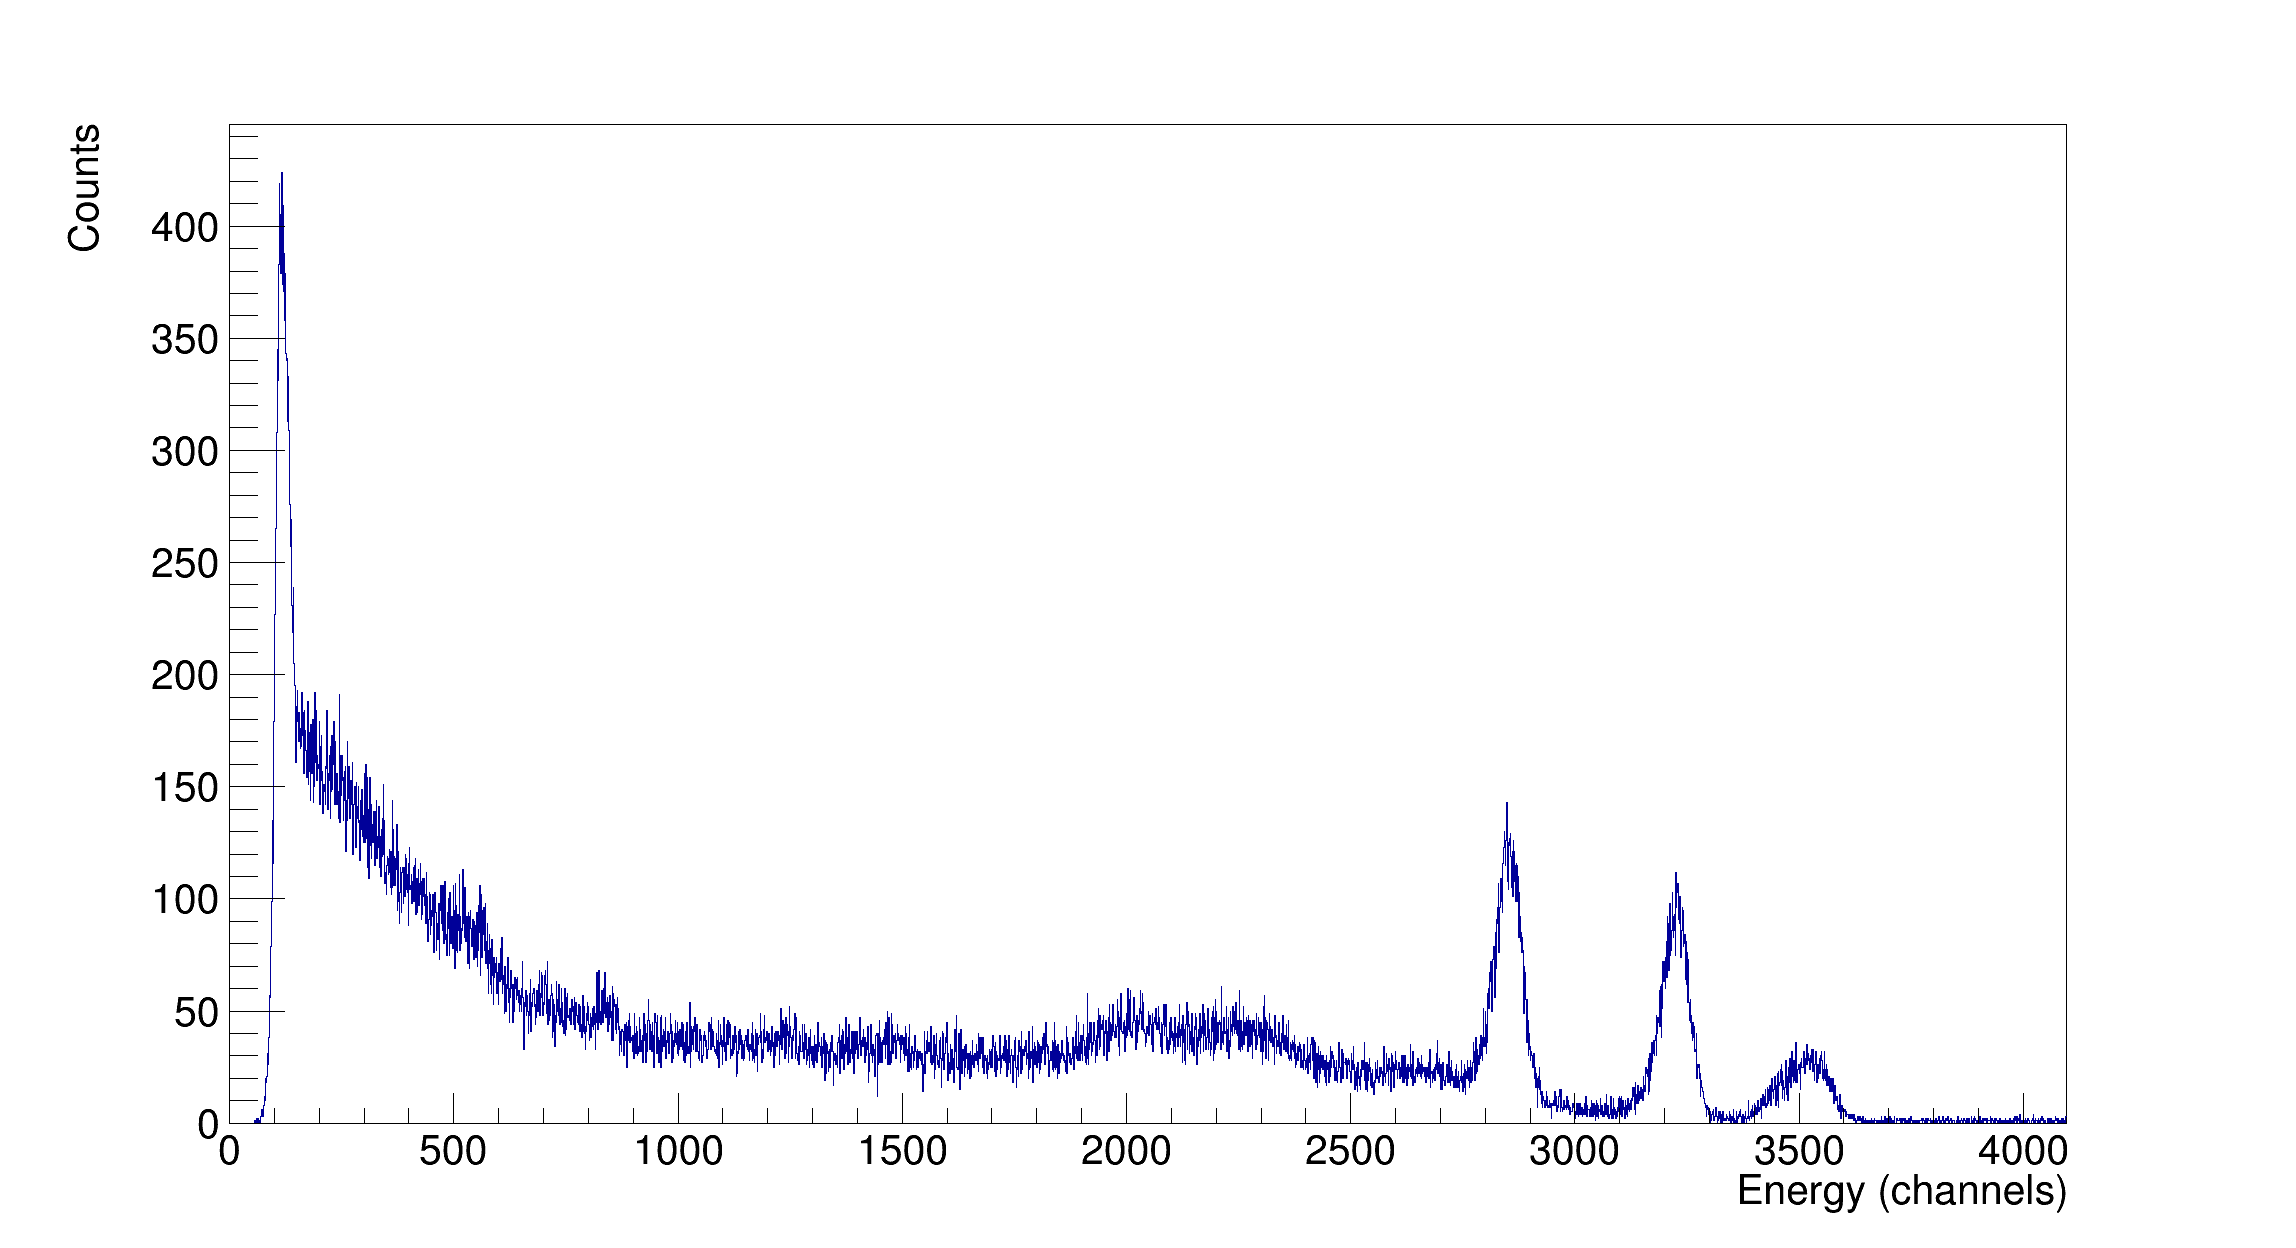
\includegraphics[width=0.80\textwidth]{labr_co60_calibration.png}
	\caption{LaBr1 response to \textsuperscript{60}Co calibration source.}
	\label{labr_co60_calibration}
\end{figure}

\subsection{MONSTER}
To measure the time of flight of neutrons produced by \an reactions, we use MONSTER, a liquid organic scintillator.
Two smaller, liquid organic TADEO scintillators were also used, but their data has not been analyzed due to their poorer efficiency.
\\

Their operating principle is the similar to that of inorganic scintillators described before, except that the excited stated that emit the \textit{scintillating} light are molecular in nature, not atomic.
Organic scintillators have a higher efficiency when for detecting neutrons than inorganic ones, as neutrons excite the material mostly through $\left( \text{n},\text{p}  \right)$ reactions (unlike gamma rays), which have a higher cross-section with hydrogen atoms.

Because the molecules are being excited by different charged particles, different states are populated and scintillating light is emmited with longer half-lifes.
This means that the resulting electric pulse is wider, which allow us to differentiate between pulses caused by photons and those caused by neutrons.
This is called \textit{pulse shape discrimination}, or PSD.

\begin{figure}[H]
	\centering
	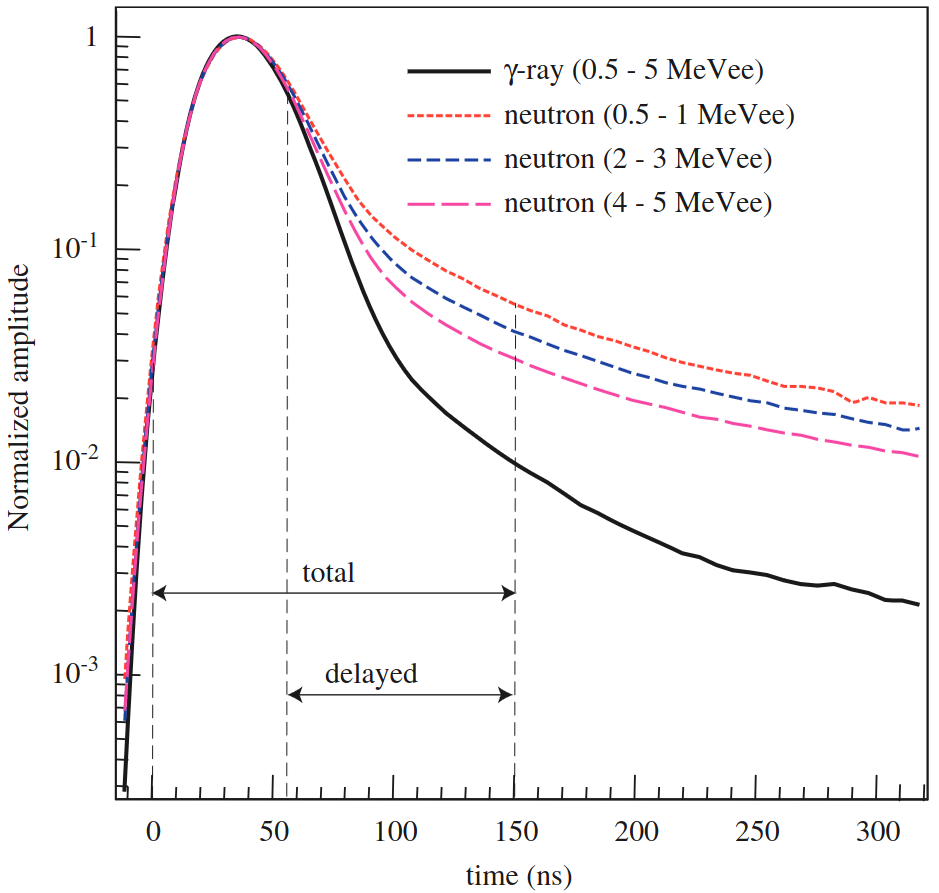
\includegraphics[width=0.35\textwidth]{psd_explanation.png}
	\caption{Illustration of scintillation pulses generated by two different radiation types.}	%TBD:mejor calidad, buscar fuente
	\label{psd_explanation}
\end{figure}

By integrating the charge in a scintillation pulse in two parts, between the initial \textit{fast} rise and the latter \textit{slow} tail, we can calculate a number, PSD:
\begin{equation}
	\text{PSD} = \frac{\text{slow}}{\text{fast}+\text{slow}}	%TBD:check
\end{equation}
that we can use to separate counts corresponding to neutrons from those that correspond to gammas.
At high energies, the \textit{fast} portion saturates, causing the sahpe seen in figure \ref{example_psd}.
This saturation can be caused either by a voltage limit in the detector or by the software in the data acquisition system.

\begin{figure}[H]
	\centering
	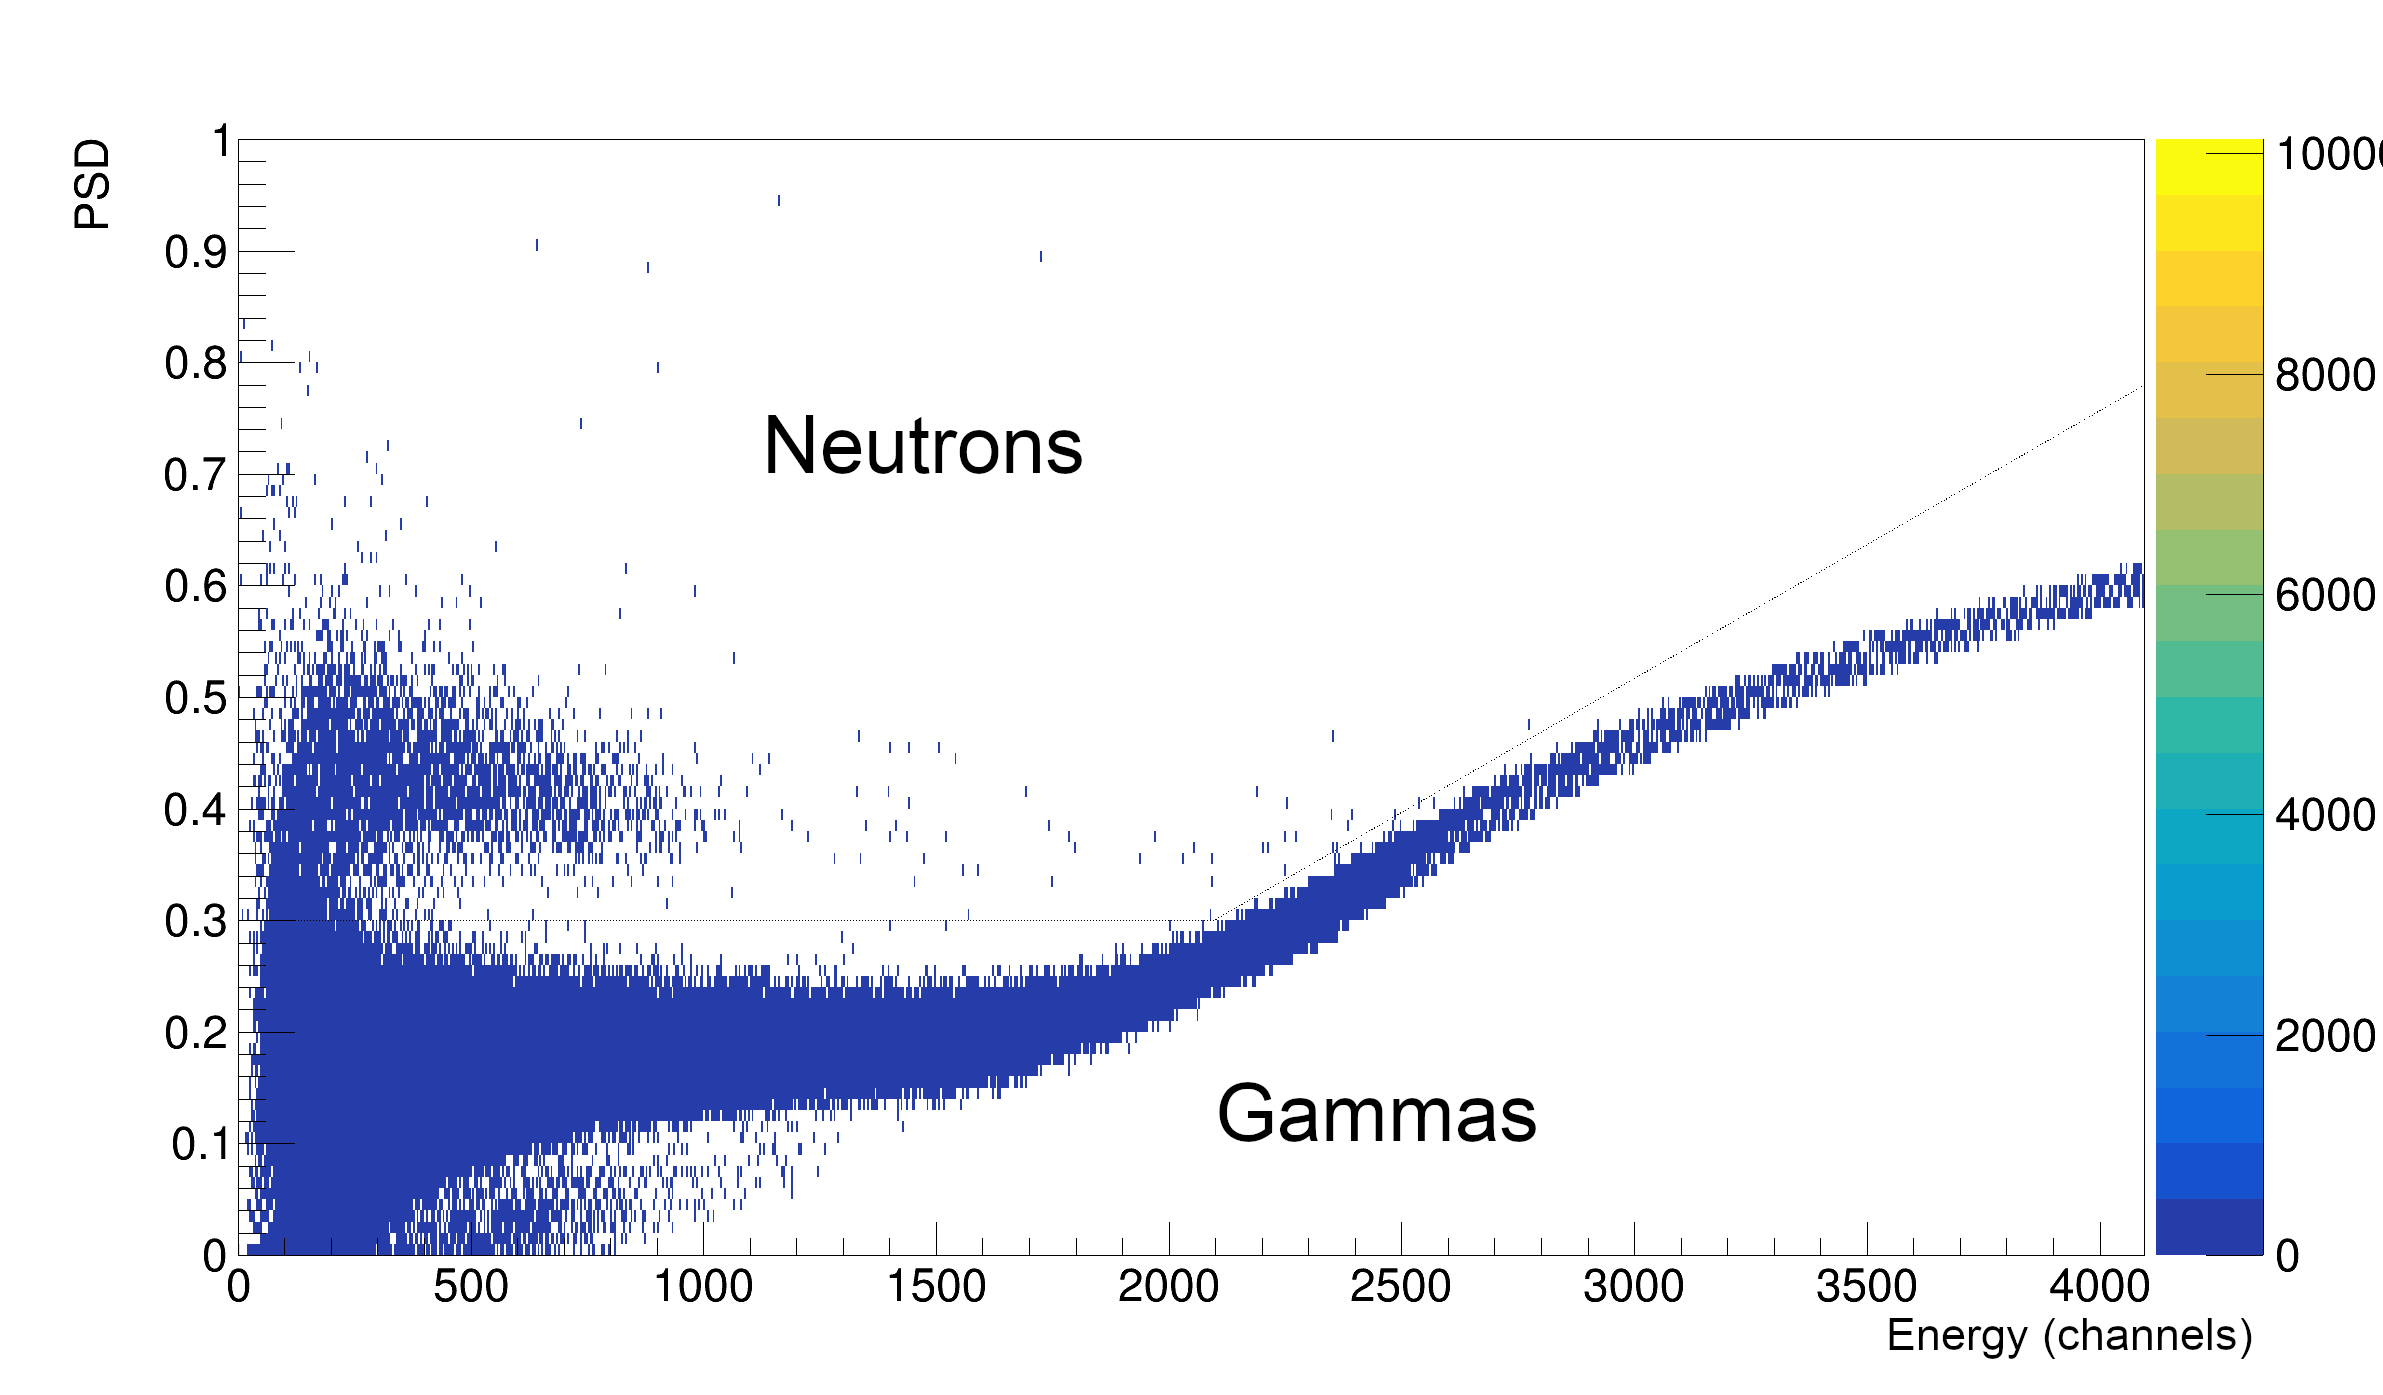
\includegraphics[width=0.80\textwidth]{example_psd.png}
	\caption{2D histogram showing PSD separation between neutrons and gamma rays for a MONSTER measurement.
	The separation line between the two is ahown in black and dotted.}
	\label{example_psd}
\end{figure}

MONSTER's response to photons is different than the lanthanum bromide detectors.
Because it is organic, the cross-section for the photoelectric effect is much smaller; and so photopeaks are not visible, only the Compton continuum is.

\begin{figure}[H]
	\centering
	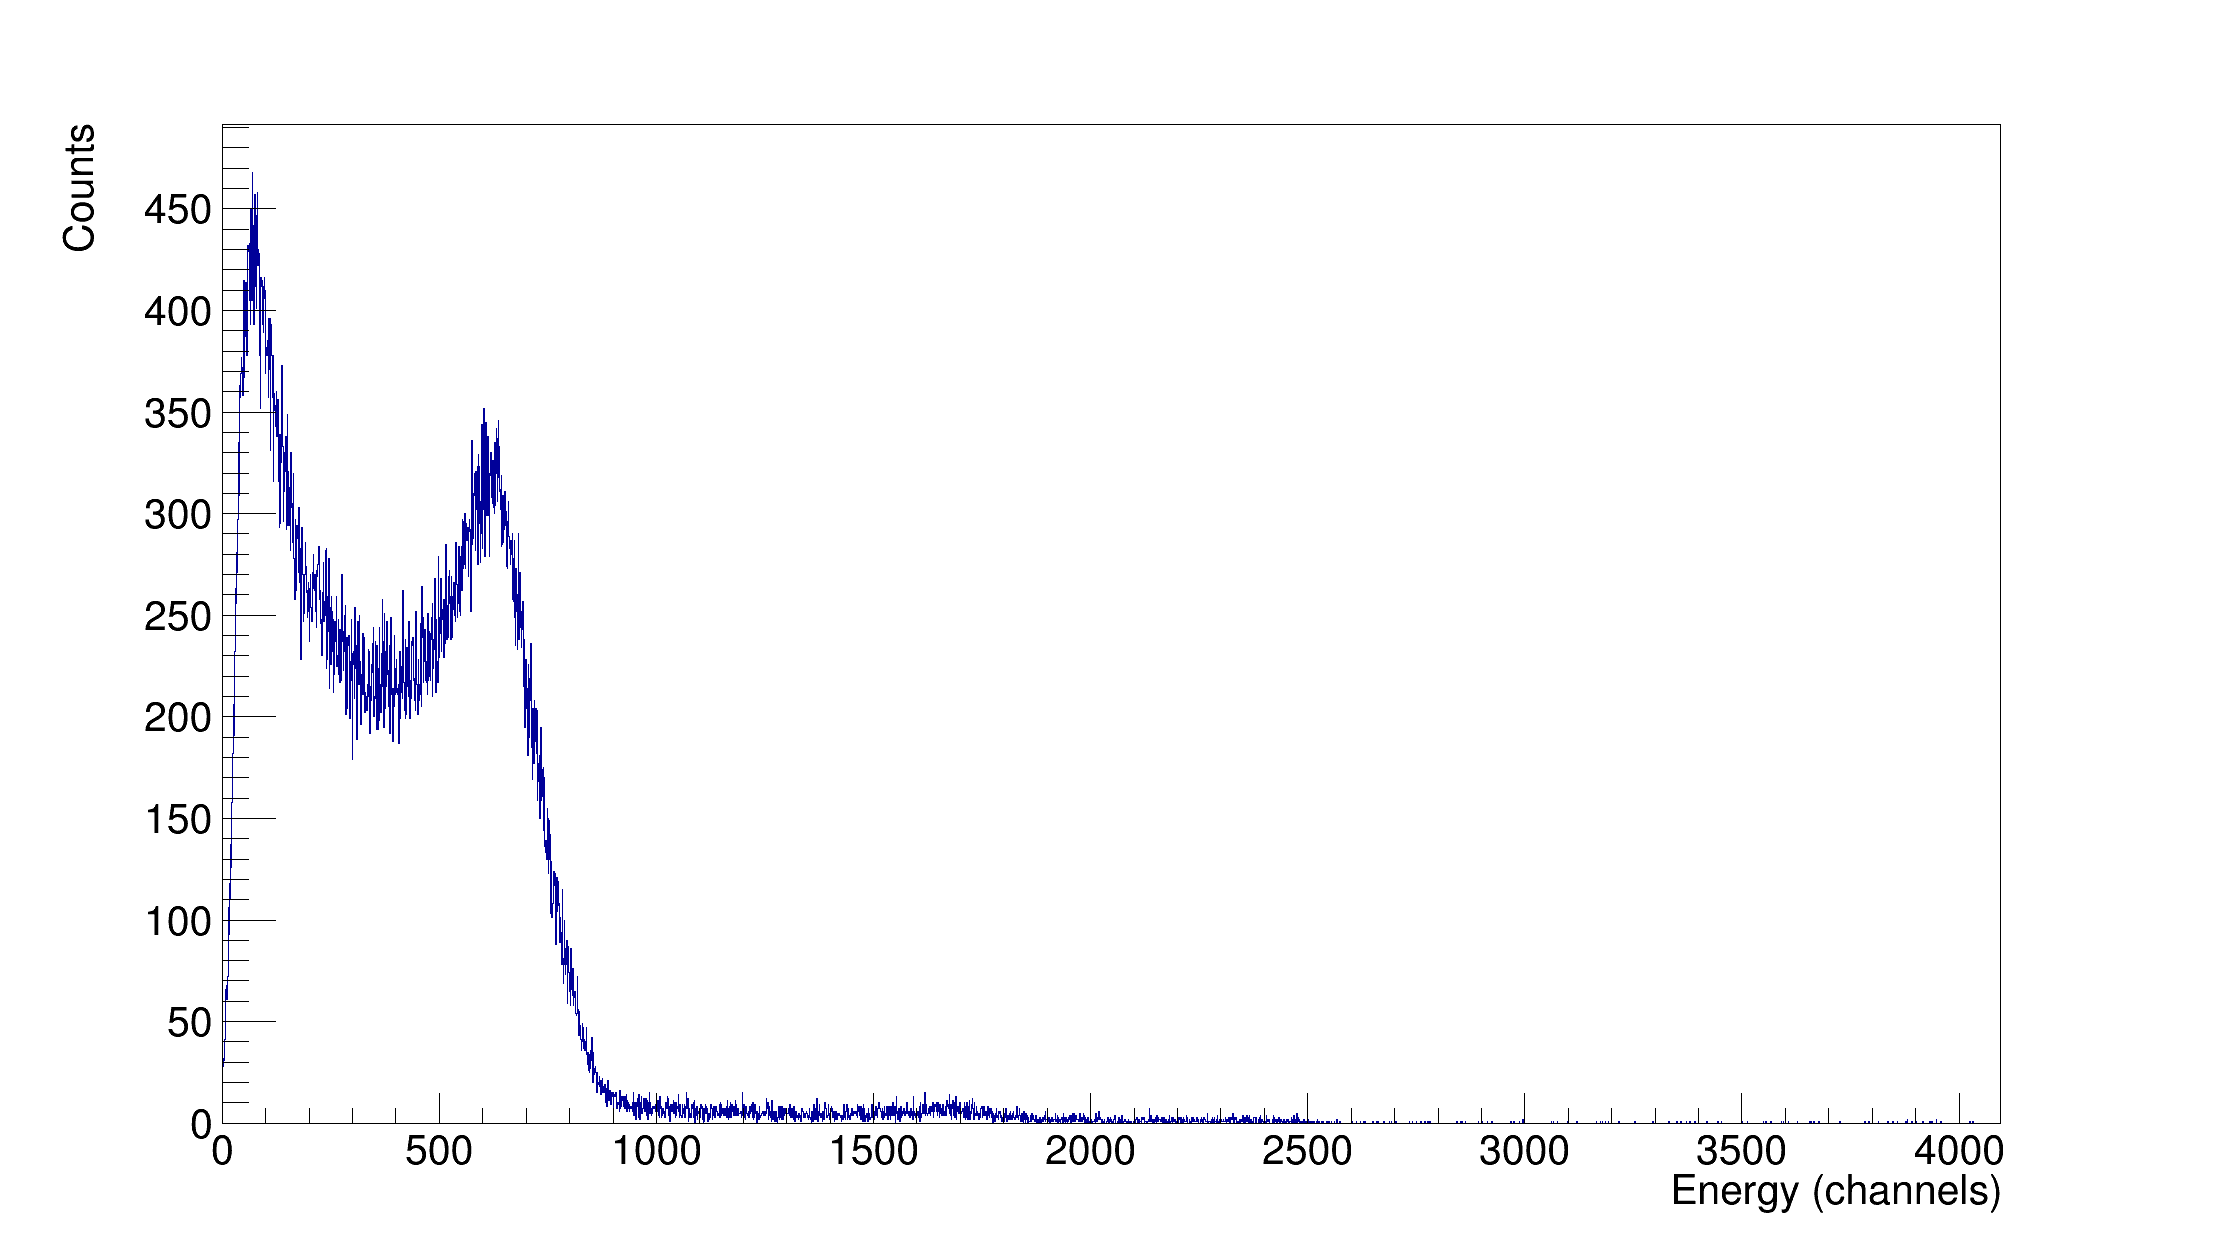
\includegraphics[width=0.80\textwidth]{monster_cs_calibration.png}
	\caption{MONSTER response to \textsuperscript{137}Cs calibration source.}
	\label{monster_cs_calibration}
\end{figure}

\begin{figure}[H]
	\centering
	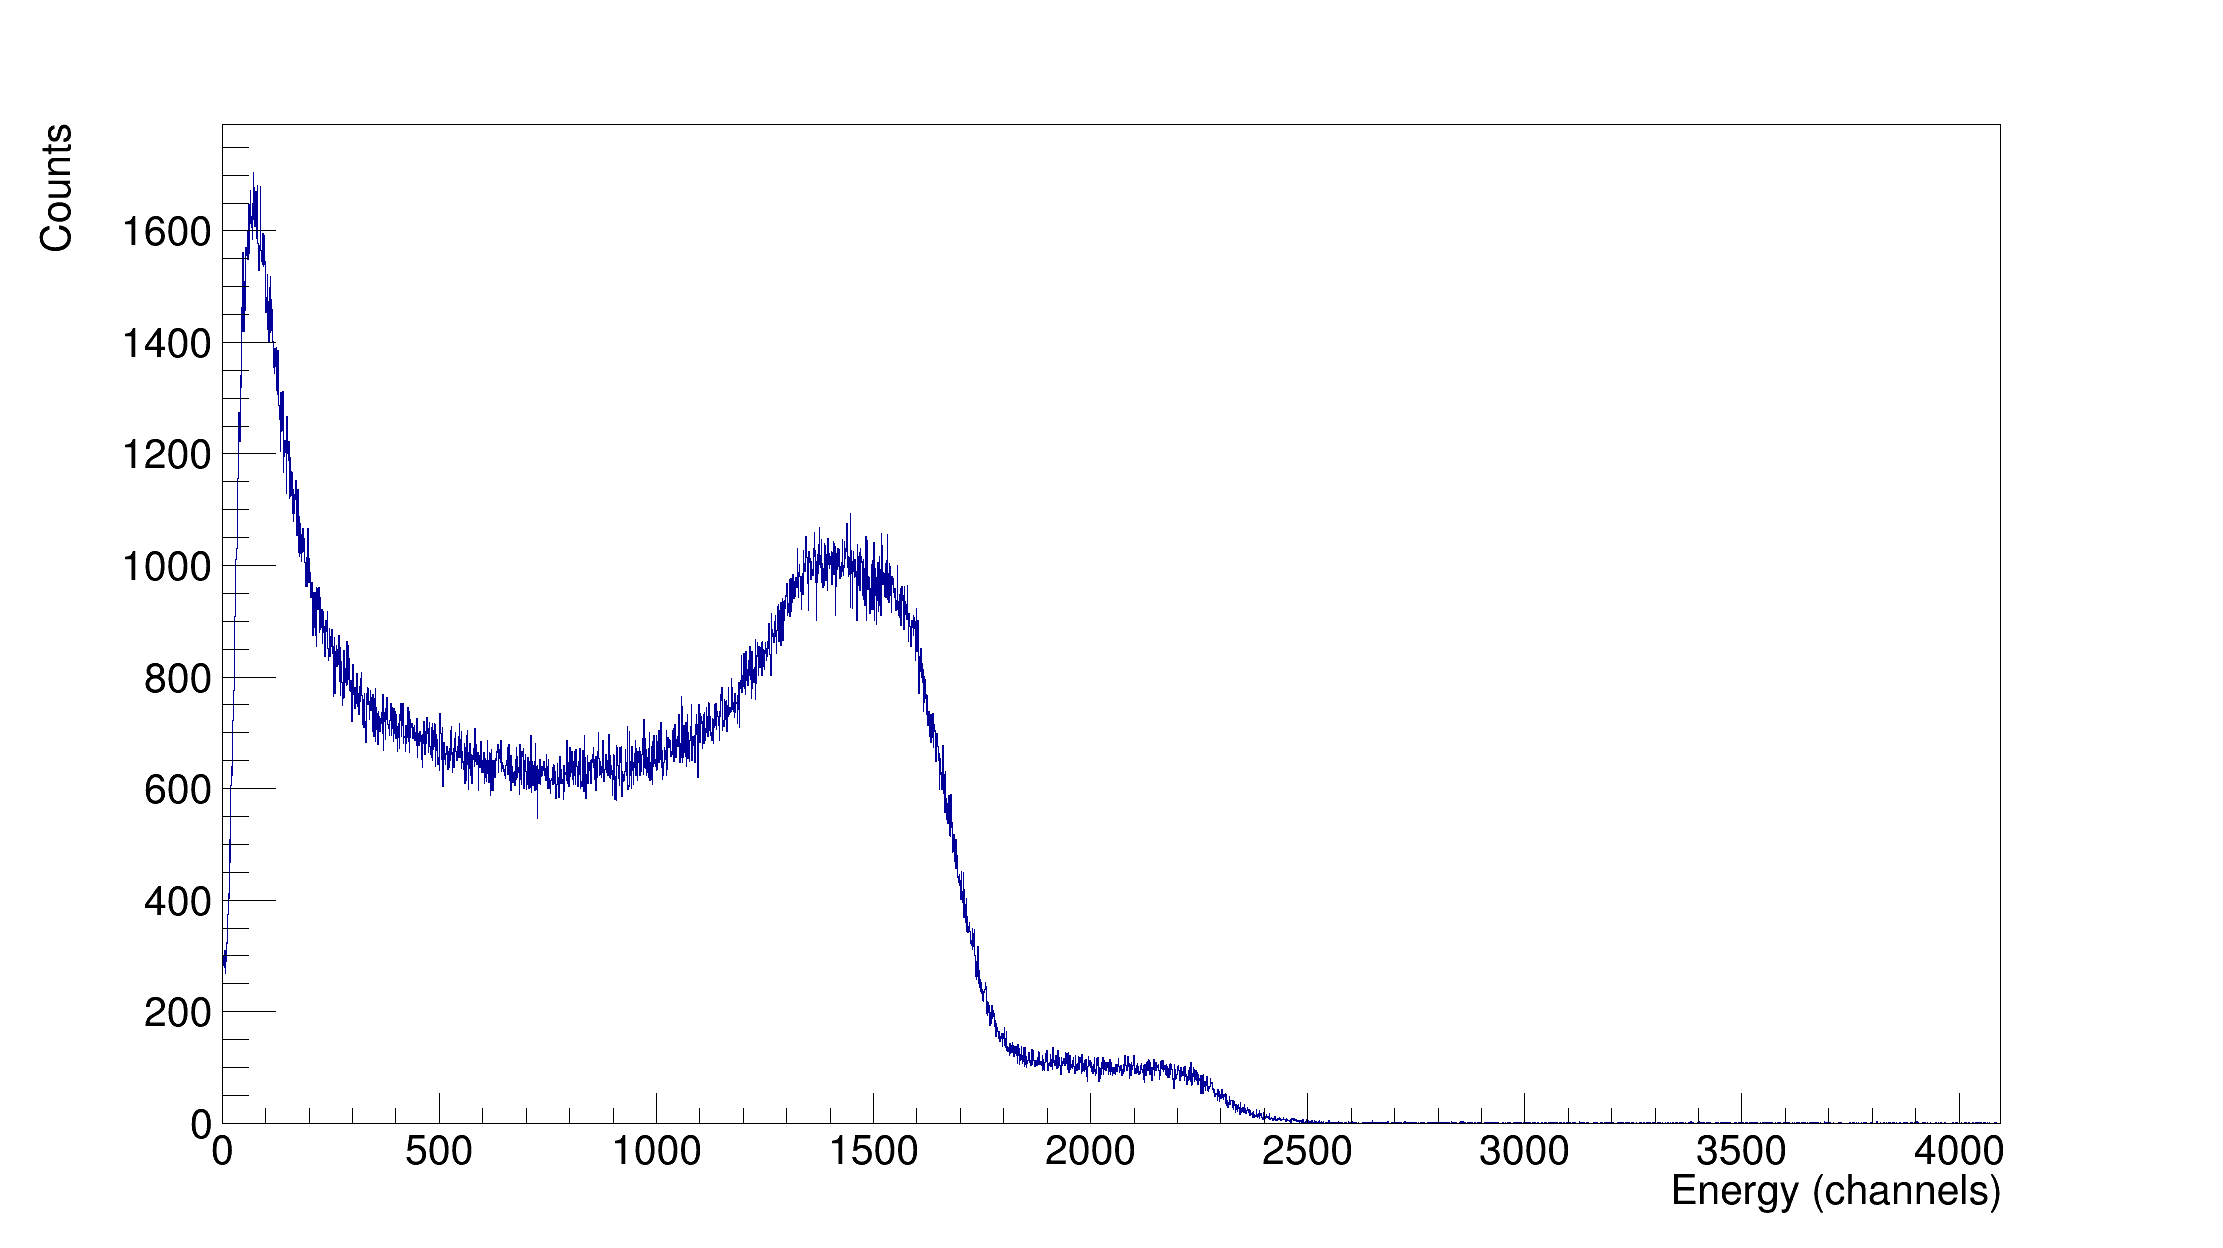
\includegraphics[width=0.80\textwidth]{monster_co_calibration.png}
	\caption{MONSTER response to \textsuperscript{60}Co calibration source.}
	\label{monster_co_calibration}
\end{figure}

To calibrate the MONSTER detector in energy, we use an efficiency curve obtained from simulations, shown in figure \ref{monster_efficiency}.	%TBD: referencia?

\begin{figure}[H]
	\centering
	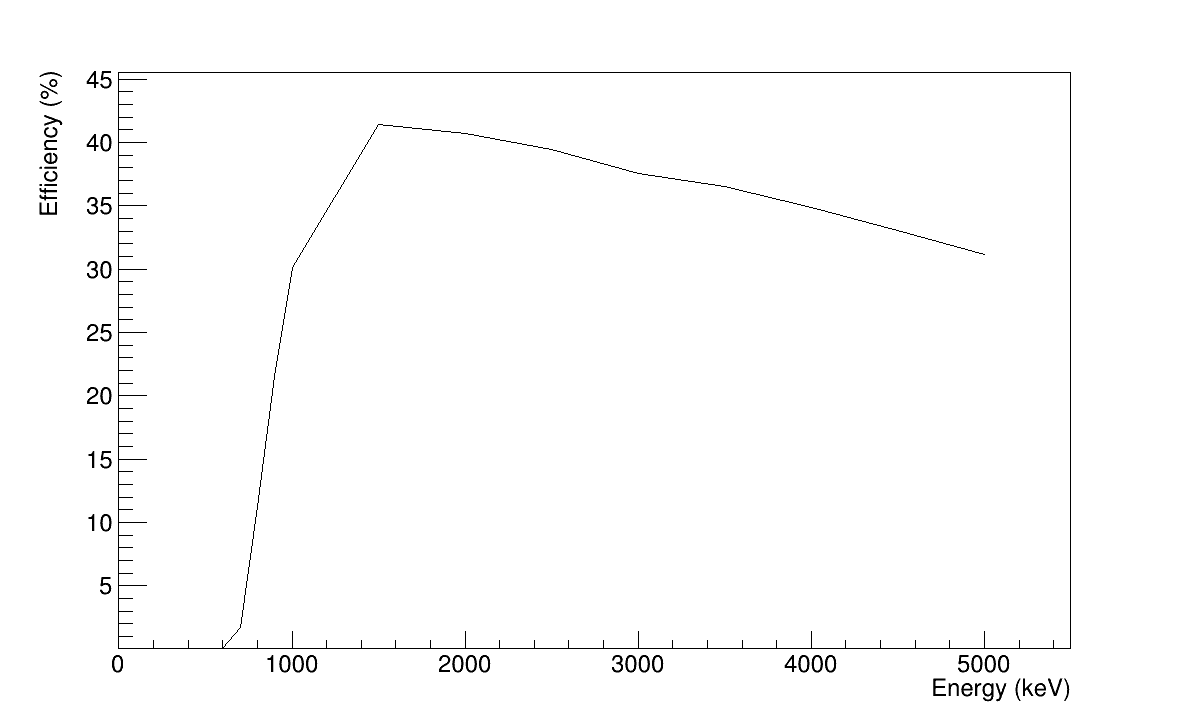
\includegraphics[width=0.80\textwidth]{monster_efficiency.png}
	\caption{MONSTER neutron efficiency curve.}
	\label{monster_efficiency}
\end{figure}

\section{DAQ}

%%%
%%%	ACTIVATION
%%%

\chapter{Activation}
Two different types of experiments are carried out, \textit{activation} ones to measure thick target yield; and \textit{time-of-flight} ones for neutron energy spectra.

\section{Procedure}
\textit{Activation} measurements are a way of measuring the yield of a reaction in a material by measuring the decay of a resulting isotope.

\subsection{Principle}
For \an \textit{activation} measurements, the beam is operated in continuous mode, launching a stream of alpha particles of a certain energy, $E_\alpha$.
When the particles hit the target, \an reactions (among others) occur.
Because the target is thick, meaning thick enough that all alphas will be stopped, these reaction will happen at alpha energies equal to or smaller than $E_\alpha$, as the particles lose energy in the target.

The number of \an reactions will be proportional to the number of incident alpha particles, and the proportionality constant is the \textbf{thick target yield}.
This is different from the regular \textit{yield}, which considers reactions at a single energy.
\begin{equation}
	\text{thick target yield} = \frac{\text{number of \an reactions}}{\text{number of incident alphas}}
	\label{tty_def}
\end{equation}

Because we cannot directly observe the reactions, activation measurements will instead count the number of produced nuclei by measuring their decay radiation.
For that, the reaction must produce an isotope that decays with an appropiately long half-life (not too long nor too short), and emitting radiation that we can easily detect.

The target is to be bombarded for at least a few half-lifes, and then left to decay for several more, while we measure the decay radiation with detectors.
We can calculate the number of produced nuclei, and thus the number of reactions that occured, by analysing the rate of detections of that radiation over time and the rate of incident particles.

\subsection{At CNA}
At the CNA, we use a thick \Aliso target with \qty{95}{\percent} purity.
Each \an reaction creates a single \Piso nuclei, with a \qty{2.498}{\minute} half-life.
We measure its decay to \textsuperscript{30}Si by $\beta +$, emitting \qty{511}{\keV} annihilation gamma-rays with an intensity of \num{1.9971}.\cite{nucleardatasheets}

\begin{figure}[H]
	\centering
	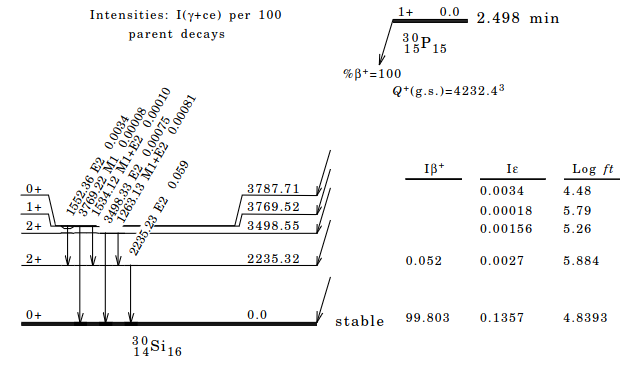
\includegraphics[width=0.7\textwidth]{Piso_decay_scheme.png}
	\caption{\Piso decay scheme.
	From \cite{nucleardatasheets}.}
	\label{Piso_decay_scheme}
\end{figure}

We irradiate the \Aliso target for several half-lifes, then the current in the accelerator is cut.
All the while the number of alphas hitting the target over time is being measured and sent to the DAQ by the current integrator (figure \ref{target_photo}).
The \Piso is then left to decay for several half-lifes.

\begin{figure}[H]
	\centering
	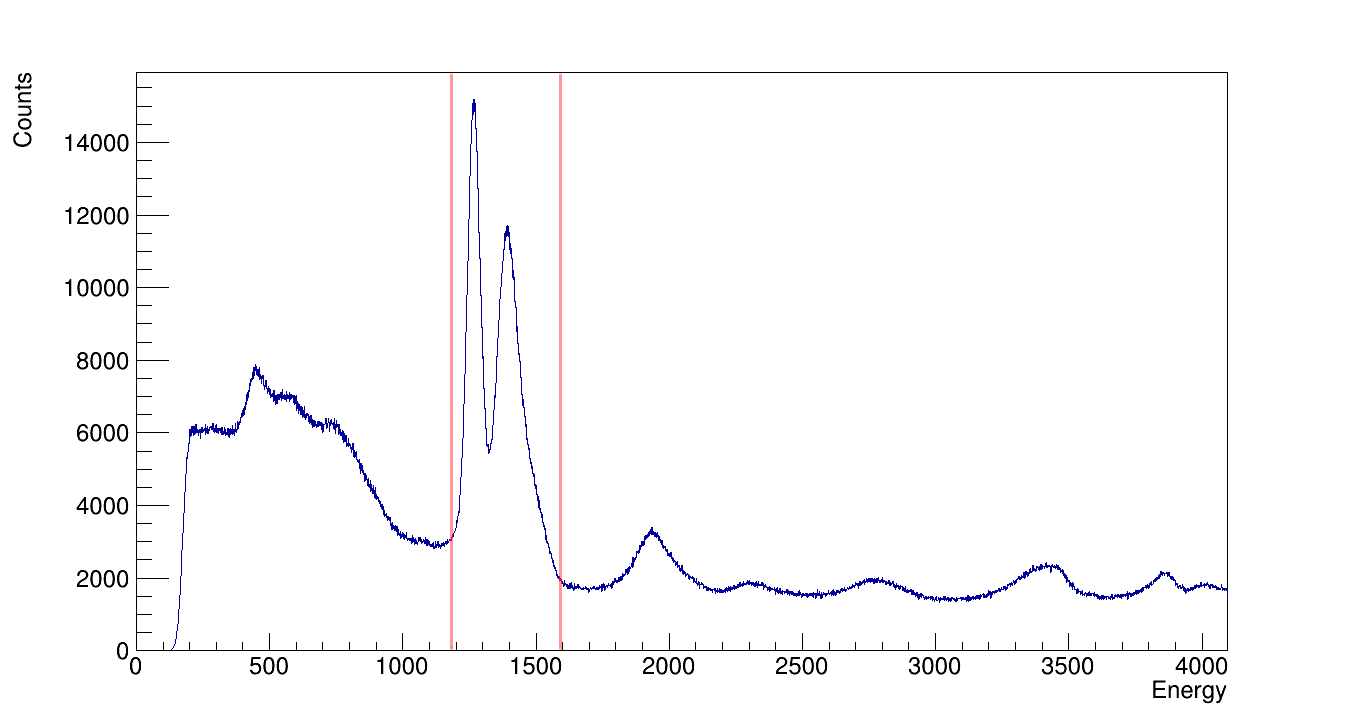
\includegraphics[width=0.80\textwidth]{example_activation_energy_histogram.png}
	\caption{Example activation spectrum.
	The energy window used to generate the time histogram (figure \ref{example_activation_time_histogram}) is shown in red.}
	\label{example_activation_energy_histogram}
\end{figure}

To measure the decay of \Piso nuclei, we use the two Lanthanum Bromide scintillators and look at the \qty{511}{\keV} gamma rays emmited from the target.
Figure \ref{example_activation_energy_histogram} shows the spectrum of one of the LaBr detectors during an activation measurement.
To represent the time histogram (figure \ref{example_activation_time_histogram}), we take only the counts whose energy fall inside the energy window shown in figure \ref{example_activation_energy_histogram}.
The reason there are two peaks, instead of the single \qty{511}{\keV} peak we would expect, is that the high rate of counts during activation changes the gain of the detectors (figure \ref{example_activation_energytime}), shifting the channel the peak corresponds to.

\begin{figure}[H]
	\centering
	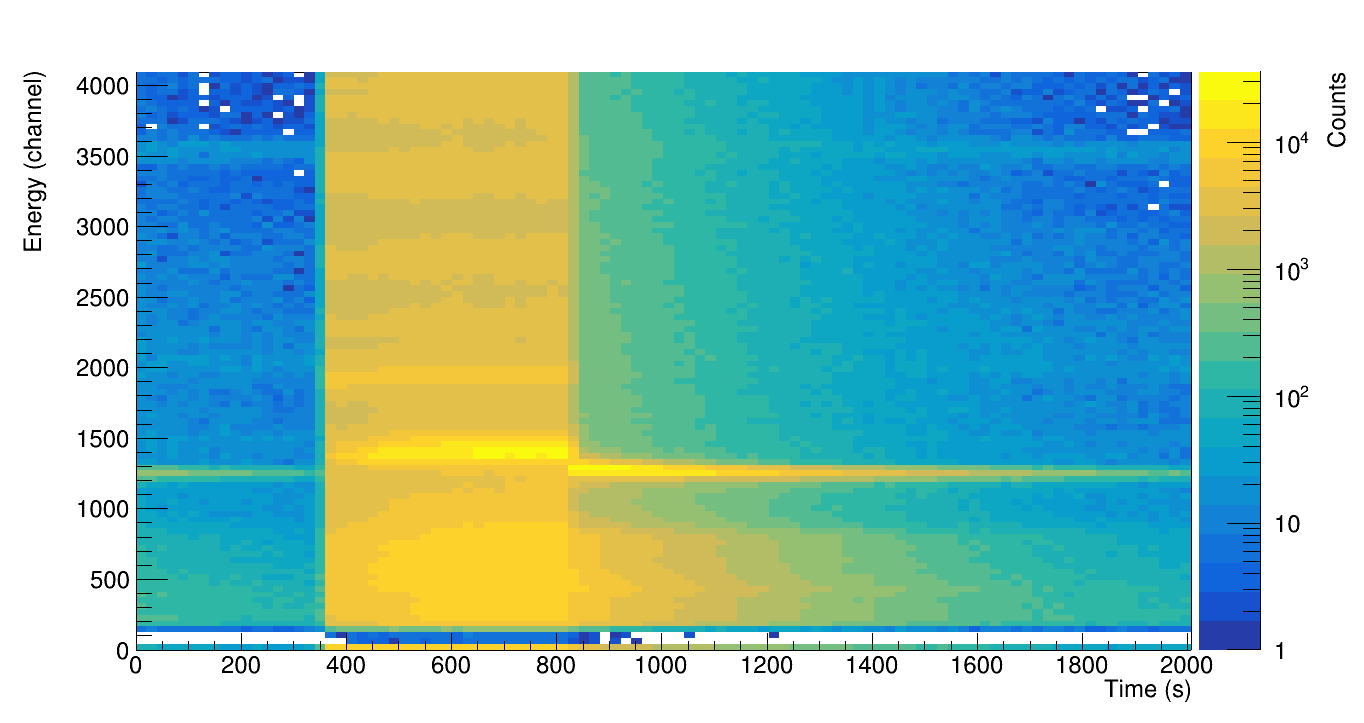
\includegraphics[width=0.80\textwidth]{example_activation_energytime.png}
	\caption{Example activation spectrum over time.
	The change in energy channel for the \qty{511}{\keV} peak is labelled in black.}
	\label{example_activation_energytime}
\end{figure}

\begin{figure}[H]
	\centering
	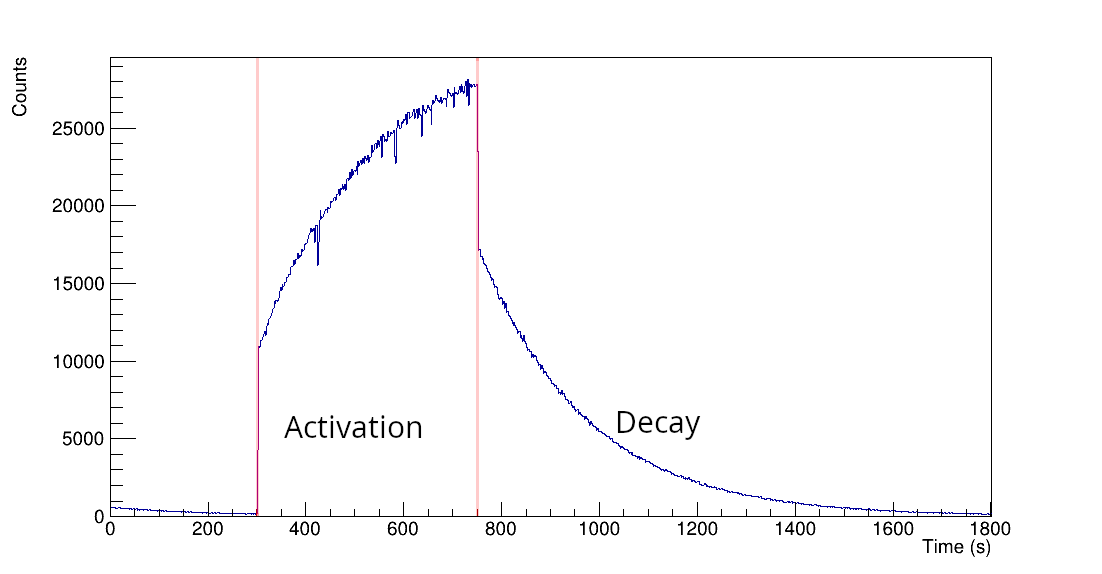
\includegraphics[width=0.80\textwidth]{example_activation_time_histogram.png}
	\caption{Example activation time histogram.
	The activation and decay periods are labeled and separated from the rest of the histogram by red lines.
	The approximate size of the \textit{extra background} caused by the alpha stream is also shown.}
	\label{example_activation_time_histogram}
\end{figure}

The time histogram in figure \ref{example_activation_time_histogram} shows initial counts before the activation starts, corresponding to decay of \Piso from the previous measurement.
When the activation starts, \num{\approx 11000} counts per bin appear very quickly.
These counts go away as soon as the activation period ends.

We call these counts the \textit{extra background}.
They are proportional to the alpha current, and correspond to gamma rays created by reactions other than \an.
They can also be seen in figure \ref{example_activation_energytime}, as the large number of counts appearing during activation well outside of the \qty{511}{\keV} peak.
They affect the histogram because, even if the emitted gammas are outside of the energy window, their Compton continuum still falls inside.

After activation ends, the counts we get correspond to the decay of the created \Piso nuclei.

\subsection{Measurements}
Activation measurements were carried out in two sessions of two consecutive days, in February and April.
Table \ref{activation_measurements_table} summarises the different measurement conditions.

Because detectors were unmounted in between both sessions, calibration measurements with \Na to determine detector efficiency (for activation measurements) were done for each detector configuration.
However, only one set of calibration measurements were done each month.
This caused problems for the April measurements, as the calibrations were done on the 18\textsuperscript{th}, but one of the detectors was moved closer for number 6, then back the following day.

\begin{table}[H]	%Tabla con datos de las medidas de activación
\centering
\begin{tabular}[c]{>{\bfseries}r||c|c|c|c}
	N & Energy (\unit{\keV}) & Current (\unit{\nano\A}) & Activation time (\unit{\s}) & Date\tablefootnote{All took place in 2023.} \\ \hline
	1	&\num{5500}&\num{128}&\num{867}&Feb 22nd\\ \hline
	2	&\num{7000}&\num{101}&\num{981}&Feb 22nd\\ \hline
	3	&\num{8500}&\num{128}&\num{909}&Feb 22nd\\ \hline
	4	&\num{8500}&\num{192}&\num{899}&Feb 23rd\\ \hline
	5	&\num{5500}&\num{123}&\num{605}&Apr 17th\\ \hline
	6	&\num{5500}&\num{312}&\num{599}&Apr 17th\\ \hline
	7	&\num{8250}&\num{193}&\num{452}&Apr 18th\\ \hline
	8	&\num{7000}&\num{216}&\num{466}&Apr 18th\\ \hline
	9	&\num{5500}&\num{151}&\num{451}&Apr 18th\\ \hline
	10	&\num{7500}&\num{183}&\num{448}&Apr 18th\\ \hline
\end{tabular}
\caption{Activation measurements}
\label{activation_measurements_table}
\end{table}

\section{Data analysis}
We can describe the number of \Piso nuclei in the target, $N$, using the differential equation:
\begin{equation}
	\ddt{N} = P(t) -\lambda N
	\label{activation_diffeq}
\end{equation}
where $\lambda$ is the decay constant of \Piso and $P(t)$ is the number of \Piso nuclei produced (by \an reactions) per unit of time, and will be proportional to the current of alphas hitting the target.
If expressed in number of alphas per second, the proportionality constant will be the thick target yield of the reaction: the number of \an reactions per incident $\alpha$ particle:
\begin{equation}
	P(t) = \text{\an reactions per unit of time} = \text{thick target yield} \cdot \text{incident alphas per unit of time}
\end{equation}
or, for an activation of duration $\Delta t$:
\begin{equation}
	\int_{\Delta t}P(t) \dif t = \text{total \an reactions} = \text{thick target yield} \cdot \text{total incident alphas}
\end{equation}
and thus:
\begin{equation}
	\text{thick target yield} =
	\frac{P(t)}{\text{incident alphas per unit of time}} =
	\frac{\int_{\Delta t}P(t) \dif t}{\text{total incident alphas}}
	\label{tty_fromP}
\end{equation}
\\

Our goal being to get the thick target yield from $P(t)$, what we will actually analyze is the activity of \Piso nuclei as they decay by $\beta +$, which will be $A = \lambda N$.
We don't actually measure the activity directly, but rather the activity times \num{1.99}: the intensity of the \qty{511}{\keV} emission.	%TBD: referencia para intensidad, tipo de decay

In order to do that, we use the two LaBr scintillators to detect \qty{511}{\keV} gamma rays.
Some counts will be noise, corresponding not to \Piso decays, but to the Compton continuum of higher energy emissions either in the environment or due to other reactions caused by the alphas in the target.
This background will have to be removed, and its value determined by the different fitting methods below.

We must take into account that, when representing the counts in a histogram, the number shown is dependent on the width of the bins.
This means that, in order to get the activity in decays per second, we must divide the \qty{511}{\keV} counts shown in a histogram by \num{1.99} and by the histogram binwidth:
\begin{equation}
	A = \text{\Piso decays per second} = \frac{\text{\qty{511}{\keV} counts per bin}}{\text{binwidth in seconds}\cdot\num{1.99}} - \text{background}
\end{equation}
We use three different methods to get $P(t)$, depending on wether $P(t)$ is considered constant during the activation period or not; and on the part of the histogram being looked at.

\subsection{Decay fit}
After the activation period is over, we are left with a certain number of \Piso nuclei that will decay following a radioactive decay law.
For the \textit{decay} fit, we simply fit this part of the activation histogram to a negative exponential, $A(t) = A\textsubscript{EOA} e^{-\lambda t} + B$ to get the \Piso activity at the end of activation, $A$\textsubscript{EOA}.

The fit also considers a constant background $B$, coming from the environment.

It is implemented using the ROOT \textit{fit} method, with $A$\textsubscript{EOA}, $\lambda$ and $B$ as fit parameters.
The value of the decay constant $\lambda$ is fixed to that of \Piso, and not determined by the fit.
However, it can be unfixed so that ROOT calculates its value, both to make sure that no other isotope is being produced at significant quantities, and as a sanity check.
Because that test was successful, the parameter is fixed to the known value of $\lambda$ and following fits only return two values: the constant background $B$, and the initial activity $A$\textsubscript{EOA}.
\\

We then divide $A$\textsubscript{EOA} by $\lambda$ to get the number of \Piso nuclei at the end of activation, $N$\textsubscript{EOA}.
However $N$\textsubscript{EOA} is not the number of \Piso nuclei created by \an reactions, as some will have decayed during the activation period.
\[ \frac{A_\text{EOA}}{\lambda} = N_\text{EOA} \neq \int_{\Delta t}P(t) \dif t \]

\begin{figure}[H]
	\centering
	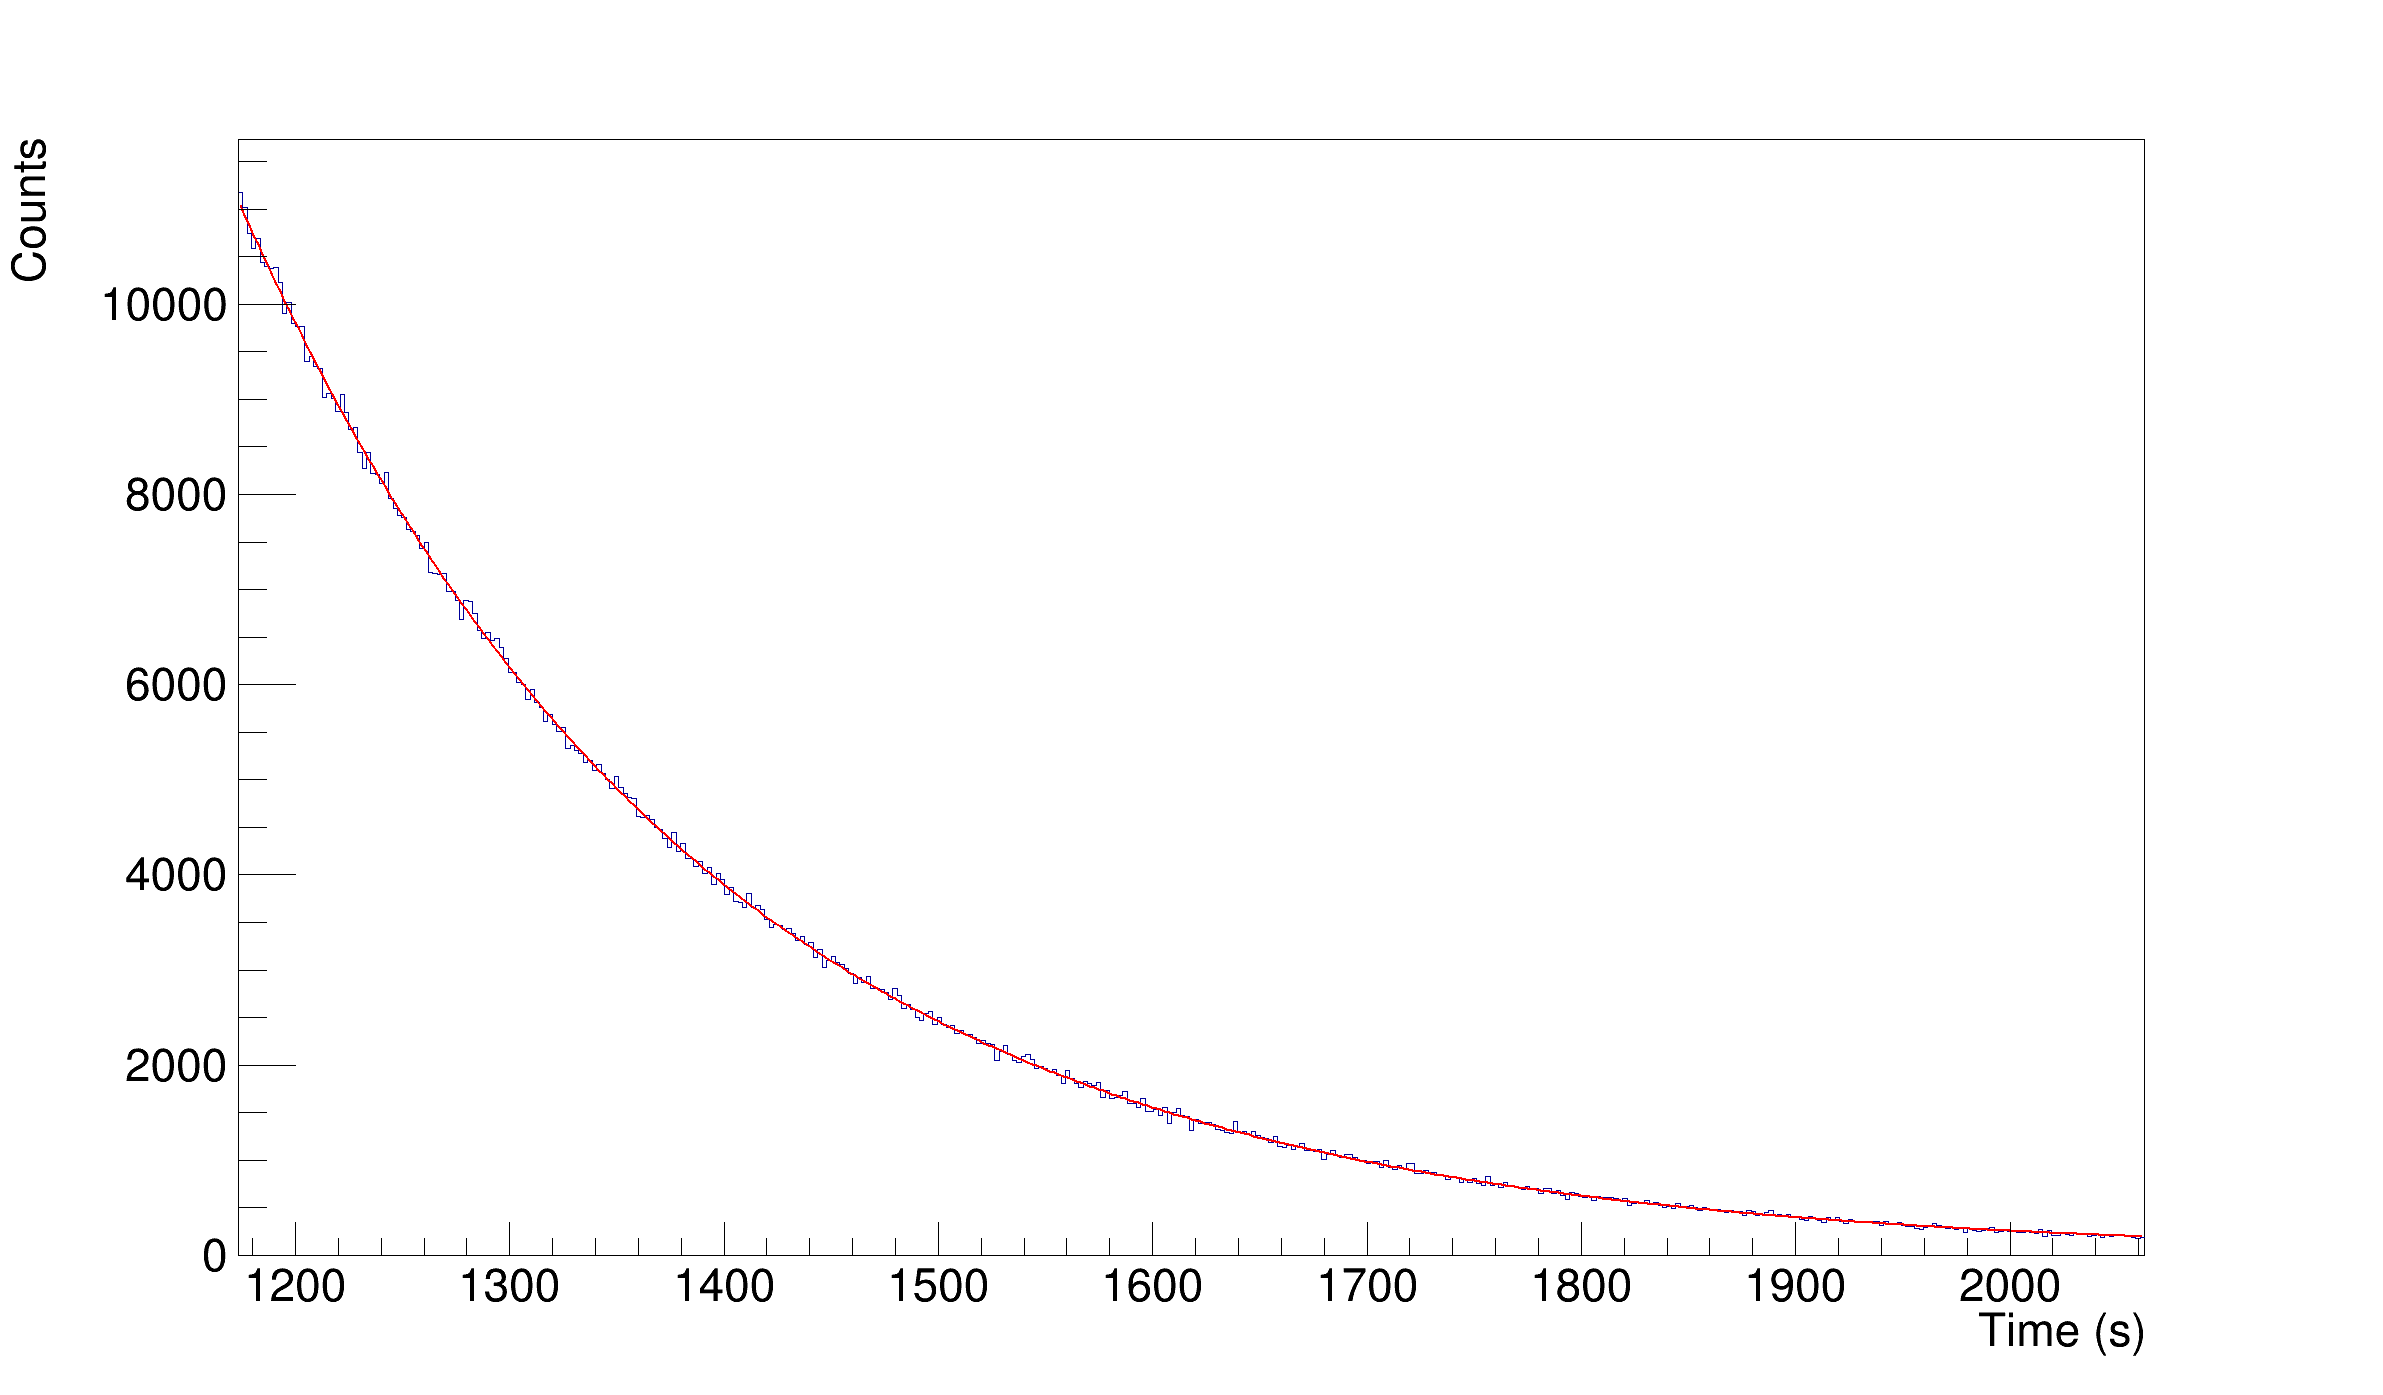
\includegraphics[width=0.80\textwidth]{example_decay_fit.png}
	\caption{Example decay fit.}
	\label{example_decay_fit}
\end{figure}

We can solve the differential equation \ref{activation_diffeq} during the activation period analytically by taking $P(t)$ as a constant, $P$.
We get
\begin{equation}
	\ddt{N} = P -\lambda N
\end{equation}
and its solution is:
\begin{equation}
	N(t) = \frac{P}{\lambda} + \left(  N_0 - \frac{P}{\lambda}  \right) e^{-\lambda t}
	\label{activation_constantP_solution}
\end{equation}
with $N_0$ the initial number of \Piso nuclei, assumed to be \num{0}.
As $t\longrightarrow\inf$, $N(t)\longrightarrow P/\lambda$, meaning production equals decay.
This effect is called \textit{saturation}, and means that, for long enough activations, one can simply take $A_\text{EOA}\approx P$.
If that approximation cannot be made (which is our case), then $N$\textsubscript{EOA} will be equal to:
\[ N\textsubscript{EOA} =N(\Delta t) = \frac{P}{\lambda} - \frac{P}{\lambda} e^{-\lambda \Delta t} = \frac{P}{\lambda} \left(1 - e^{-\lambda \Delta t} \right)\Longrightarrow A\textsubscript{EOA}=P\left(1-e^{-\lambda\Delta t}\right)\Longrightarrow \]
\begin{equation}
	P = \frac{A\textsubscript{EOA}}{1 - e^{-\lambda \Delta t}}
\end{equation}
with $\Delta t$ the total activation time.
$P\cdot\Delta t$ is the total number of \Piso nuclei created during the activation, meaning we can now get the thick target yield, according to equation \ref{tty_fromP}, as:
\begin{equation}
	\text{thick target yield} = \frac{P\cdot \Delta t}{\text{total incident alphas}} = \frac{A_\text{EOA}\cdot \Delta t}{\text{total incident alphas} \cdot \left( 1-e^{-\lambda \Delta t}  \right)}
\end{equation}

All that is left is to correct for the efficiency of the detector, and the final formula for the thick target yield is:
\begin{equation}
	\text{thick target yield} = \frac{A_\text{EOA}\cdot\Delta t}{\text{total incident alphas} \cdot \text{detector efficiency} \cdot \left(1 - e^{-\lambda \Delta t} \right)}	%TBD? use symbols instead?
\end{equation}
\\

The advantages of this method are:
\begin{itemize}
	\item The fitting is simple and fast.
	\item Only the total number of incident alphas is needed, not information of current over time.
	\item The \textit{extra background} doesn't bother us, as we only care about the counts once activation ends.
	\item It is the standard way to carry out activation measurements.
\end{itemize}
The main disadvantage is that, because it assumes $P(t)$ to be constant, the method won't work if the alpha current is not approximately constant over time.

\subsection{Unified and rise fit}
Instead of taking $P(t)$ as constant and integrating \ref{activation_diffeq} analitically, another option is to fit either the whole histogram or the activation period (\textit{unified} or \textit{rise} fits, respectively) to a function that numerically integrates equation \ref{activation_diffeq} step by step.

The function takes the data of current over time as input, and calculates $P(t)$ every step as $P(t) = \text{thick target yield}\cdot\text{alphas}$, with 'alphas' the number of incident alphas during the step.
This is useful because the current is not perfectly constant, there are drops and rises in many of the measurements (figure \ref{current_histograms}) and this could make the \textit{decay} fit less precise, as the assumption of constant current could be incorrect.
\\
\begin{figure}[H]
	\centering
	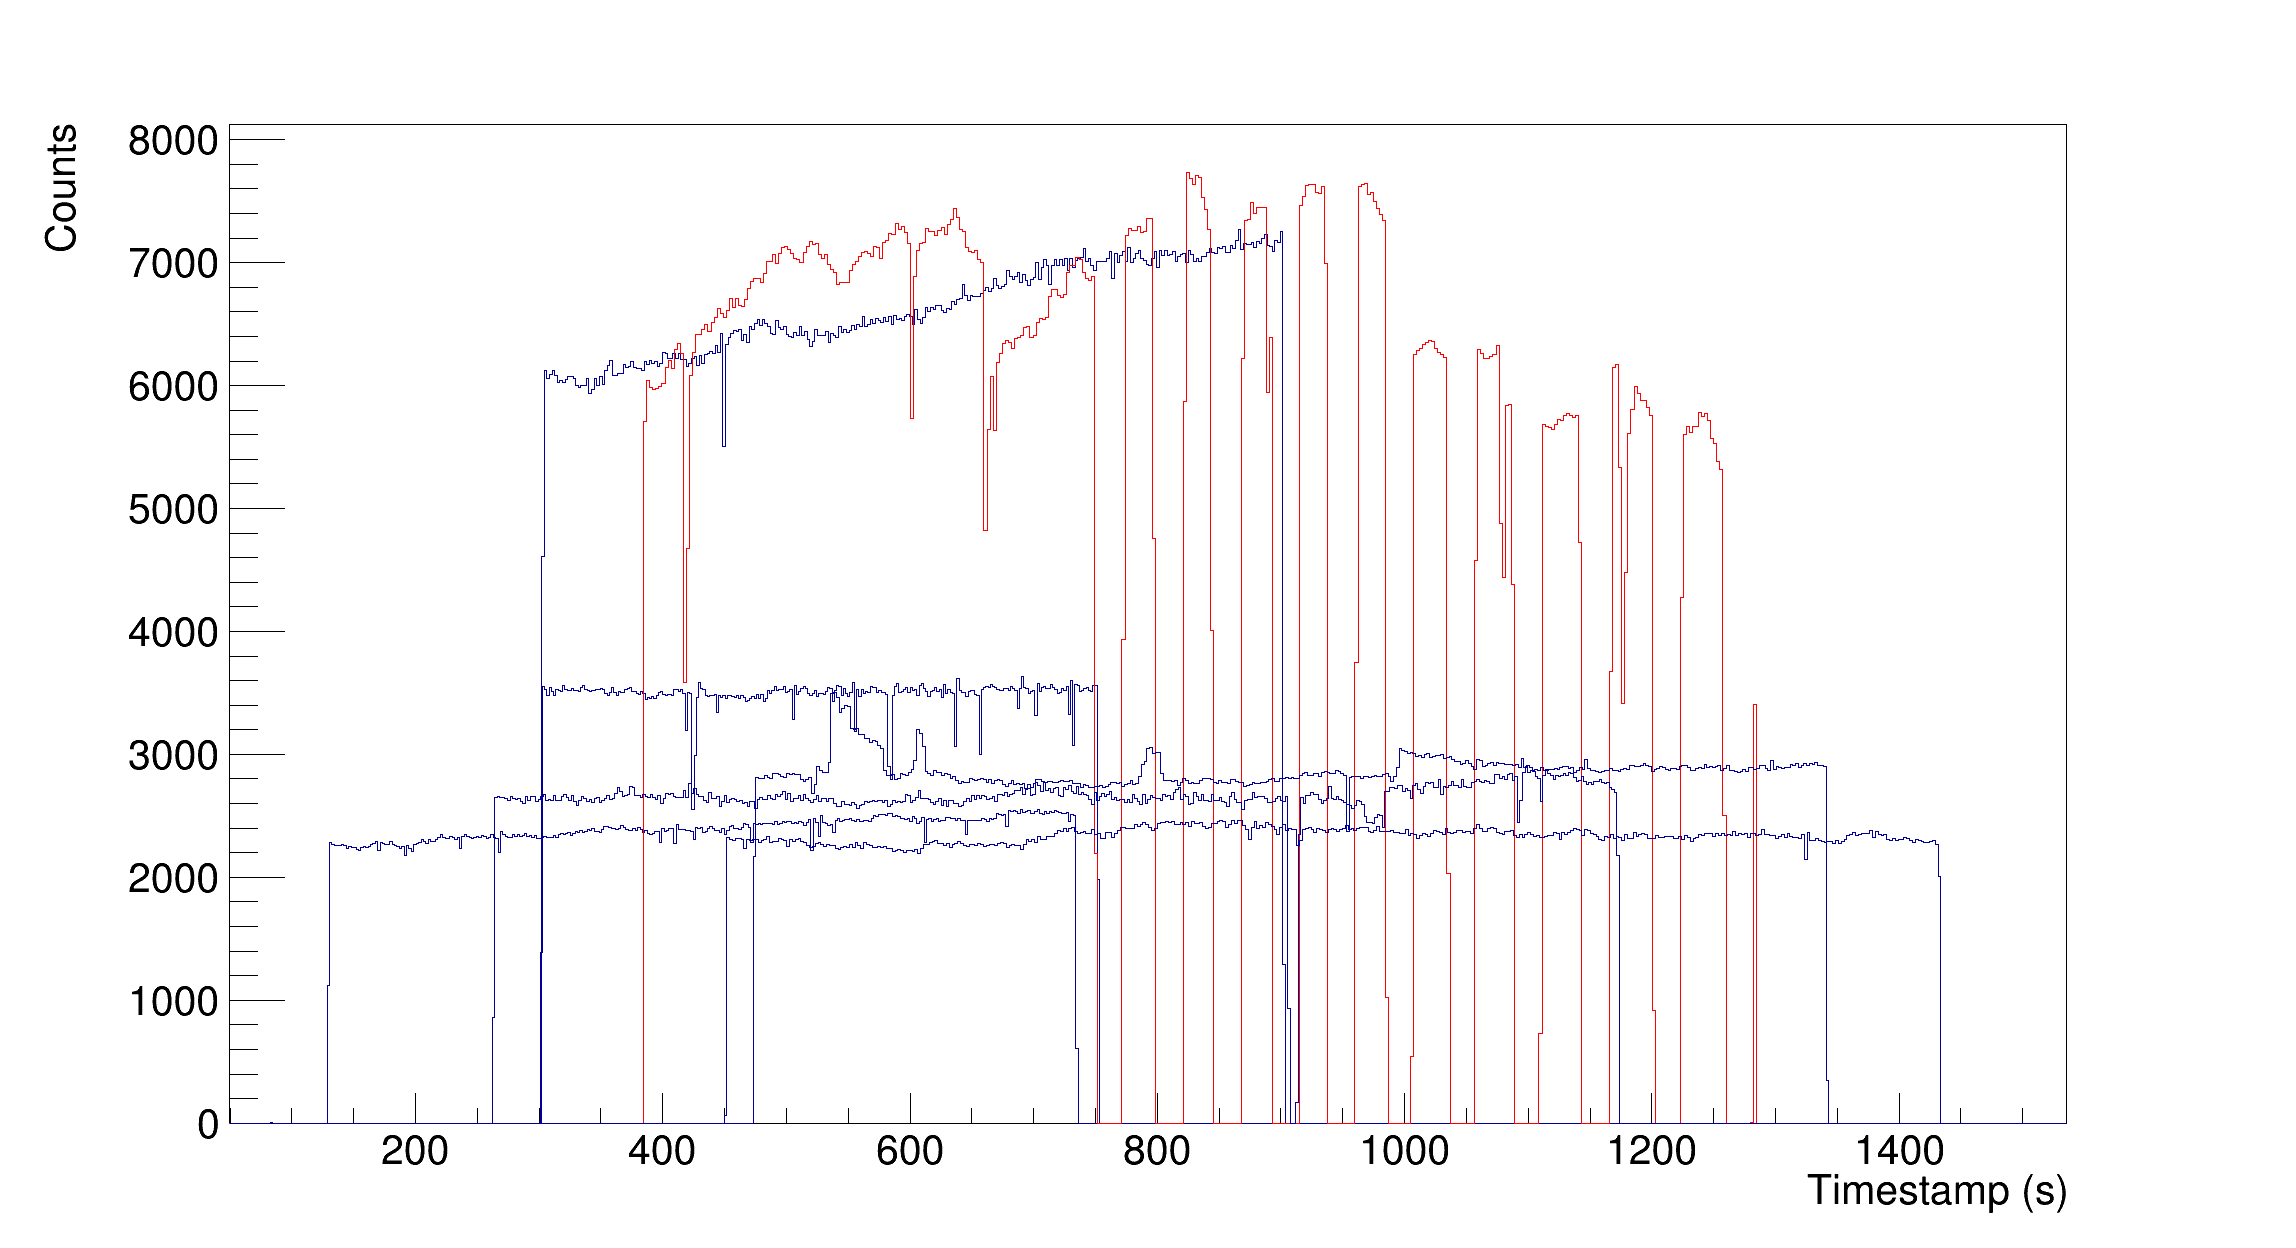
\includegraphics[width=0.80\textwidth]{current_histograms.png}
	\caption{All current histograms, superimposed.
	The one in red corresponds to measurement 4.}
	\label{current_histograms}
\end{figure}

The function is implemented using a C++ functor, and the fitting using ROOT's \textit{fit} method.
Every step, it calculates $P(t)=\text{thick target yield}\cdot\text{alphas}$, then assumes $P$ constant for the duration of the step.
It sets the new number of \Piso nuclei as:
\begin{equation}
	N(t+\dif t)=\frac{P}{\lambda} + \left( N(t)-\frac{P}{\lambda} \right) e^{-\lambda \dif t}
\end{equation}
then repeats until the end of the data.
This numerically integrates equation \ref{activation_diffeq} using the analytical solution \ref{activation_constantP_solution}.
It outputs the counts over time ($1.99 \lambda N$) every step, so that ROOT can compare it to the histogram of \qty{511}{\keV} counts over time for fitting.
The thick target yield is one of the parameters adjusted by the fitting (it is used to calculate $P$), and so it is outputted by ROOT directly and only the binwidth of the histogram needs to be acounted for.

This function also considers a constant background (adding it to its output), an initial number of \Piso (from previous activation runs); and a number of counts proportional to the current (also added to its output), which correspond to the \textit{extra background}.
All of those are also parameters for the fitting, and also adjusted by ROOT.
\\

The thick target yield, corrected by the detector efficiency, in units of \an per alpha, is:
\begin{equation}
	\text{thick target yield} = \frac{\text{result of the fitting}}{\text{detector efficiency}}
\end{equation}
with \num{1.99} the intensity of the \qty{511}{\keV} decay radiation, which we need to divide by because the histograms involved are in counts, not \Piso decays.

\begin{figure}[H]
	\centering
	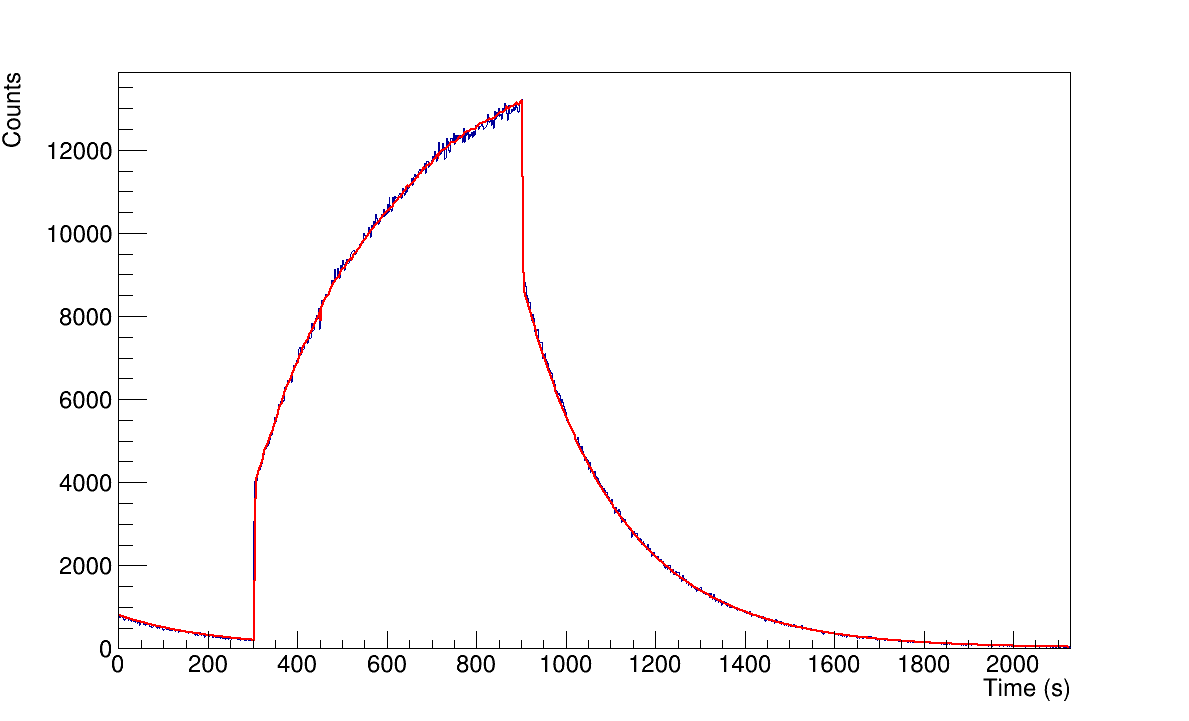
\includegraphics[width=0.80\textwidth]{example_unified_fit.png}
	\caption{Example unified fit (red) and data (blue).}
	\label{example_unified_fit}
\end{figure}

\begin{figure}[H]
	\centering
	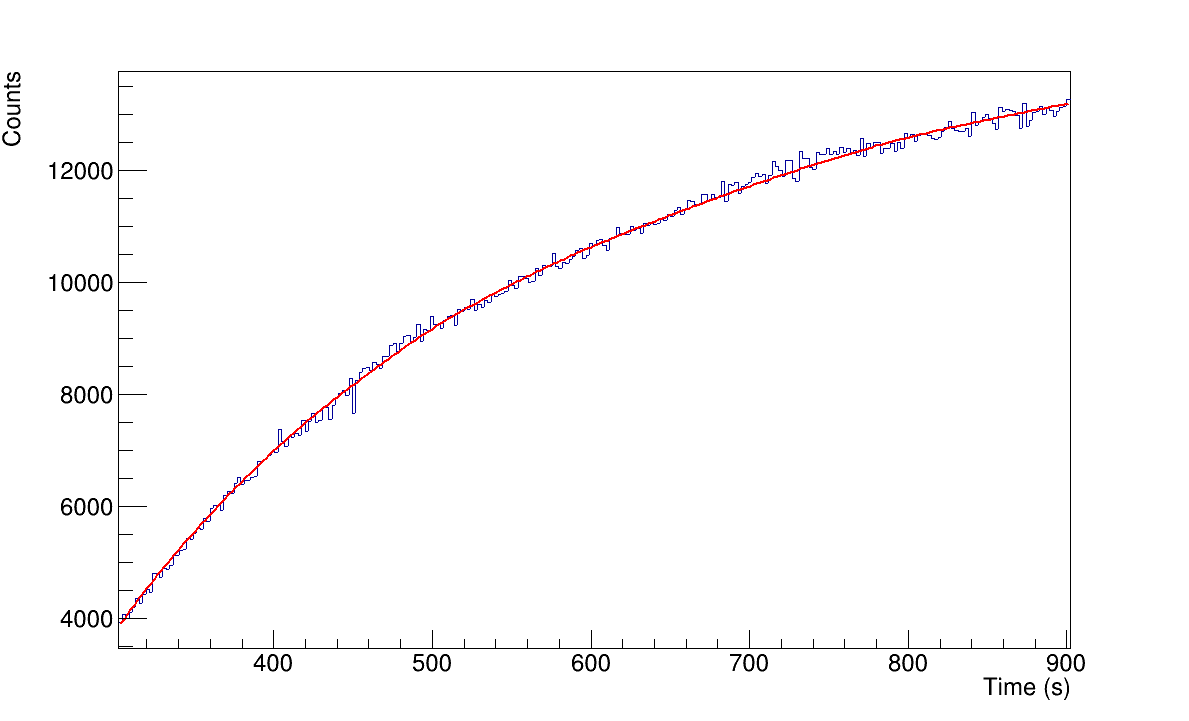
\includegraphics[width=0.80\textwidth]{example_rise_fit.png}
	\caption{Example rise fit (red) and data (blue).}
	\label{example_rise_fit}
\end{figure}

Figures \ref{example_unified_fit} and \ref{example_rise_fit} show the fits (red) to the data (blue).
We can see that they adjust very well.
In figure \ref{example_unified_fit}, we can see that it also correctly accounts for an initial amount of \Piso from a previous activation, as well as the \textit{rise} and \textit{decay} periods.
\\

Data of current over time was not recorded in half of the measurements in April (numbers 8, 9 and 10).	%TBD: por qué razón?
In addition, measurement number 4, in February, shows loss of data due to a problem with the DAQ.

\begin{figure}[H]
	\centering
	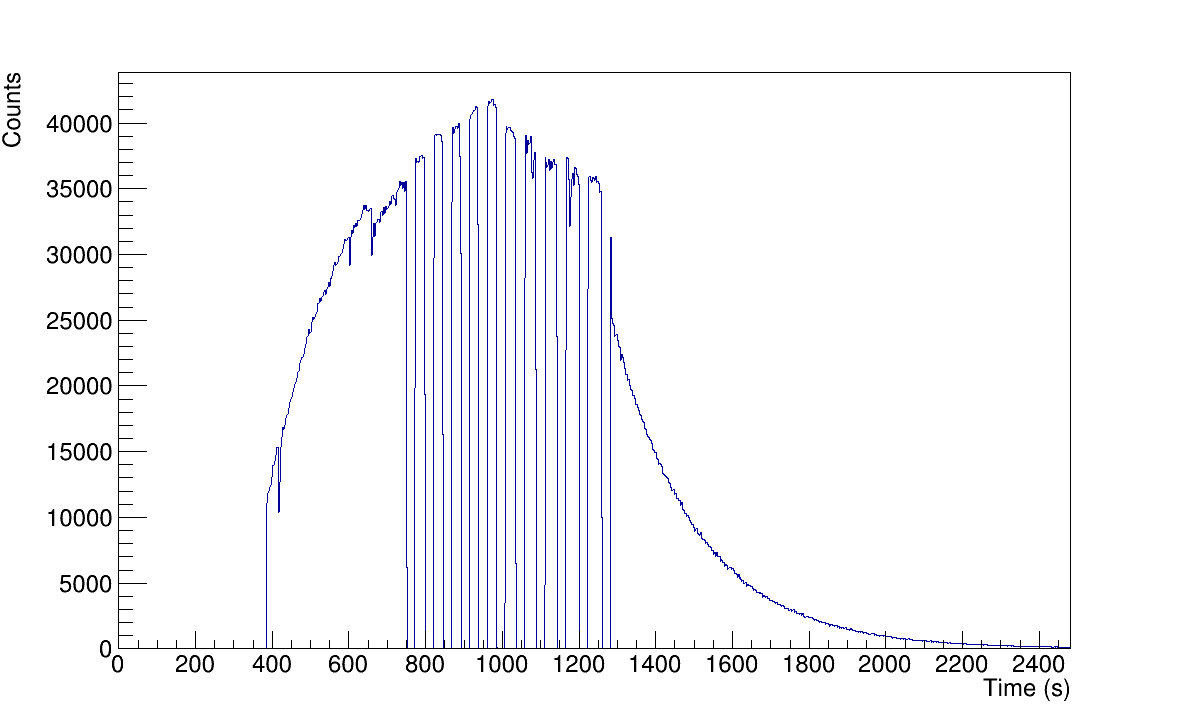
\includegraphics[width=0.80\textwidth]{activation_4_time.png}
	\caption{Activation measurement number 4.
	We can see the loss of signal to the DAQ periodically for most of the activation period.}
	\label{activation_4_time}
\end{figure}

These problems prevent the \textit{unified} and \textit{rise} fits from being used for all measurements.
\\

\section{Results}
Because all measurements were carried out with two detectors, we can start by comparing them.
Afterwards, we can compare the different methods with each other, to find out wether they agree.
Then, we can compare the final results with data from EXFOR.

\subsection{Agreement between detectors}
In theory, both detectors should give the exact same result.
Figure \ref{decay_errors_rel_per} shows that the relative difference in measurements between LaBr detectors 1 and 2 is around \qty{4}{\percent} for February and \qty{8}{\percent} for April.
The points shown are for \textit{decay} fit measurements only (for the sake of brevity), but are similar for the other methods.
The percentage is calculated as the difference between LaBr 1 and the mean, over the mean of both detectors: $\frac{\text{LaBr}_1-\text{mean}}{\text{mean}}\cdot 100 = \frac{\text{LaBr}_1-\text{LaBr}_2}{\text{LaBr}_1+\text{LaBr}_2}\cdot 100$.
This is so that it roughly corresponds to the uncertainty of the mean.

Measurements in February show negative values, indicating detector 2 is higher; while those in April are positive, meaning the opposite is true.

\begin{figure}[H]
	\centering
	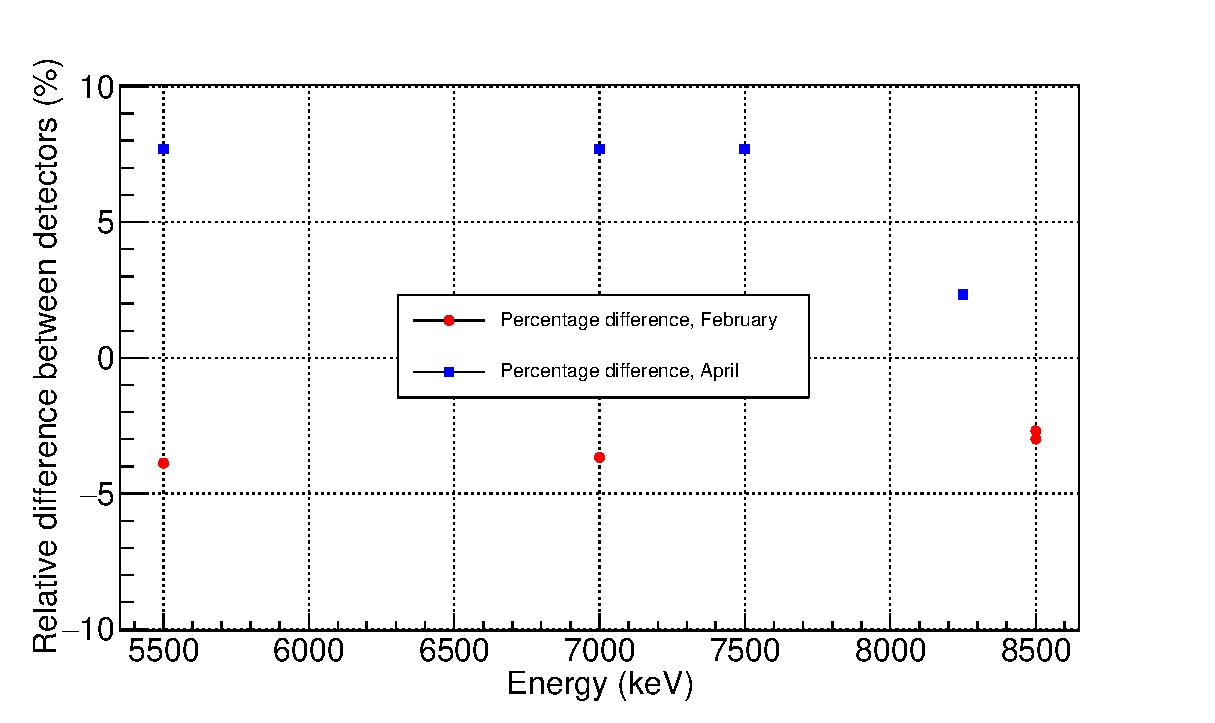
\includegraphics[width=0.80\textwidth]{decay_errors_rel_per.eps}
	\caption{Percentage difference in thick target yield results between detectors in each measurement.
	The number shown is calculated as $\frac{\text{LaBr}_1-\text{LaBr}_2}{\text{LaBr}_1+\text{LaBr}_2}\cdot 100$, the difference over the average, in percentage.}
	\label{decay_errors_rel_per}
\end{figure}

The outlier, with \qty{-30}{\percent}, corresponds to measurement number 6.
For this measurement, LaBr detector number 1 was placed much closer to the target, and at \qty{0}{\degree}.
The corresponding \Na calibration measurement does not correspond to that configuration, and so the results from this measurement and detector are unreliable.
The measurements \emph{before} the change in position can also not be trusted, as the calibration was done on the 18th, after the position was changed back; and the distances and angles were not carefully measured.

Going forward, measurements 5 and 6 will be discarded, and their results not shown.
\\

\begin{figure}[H]
	\centering
	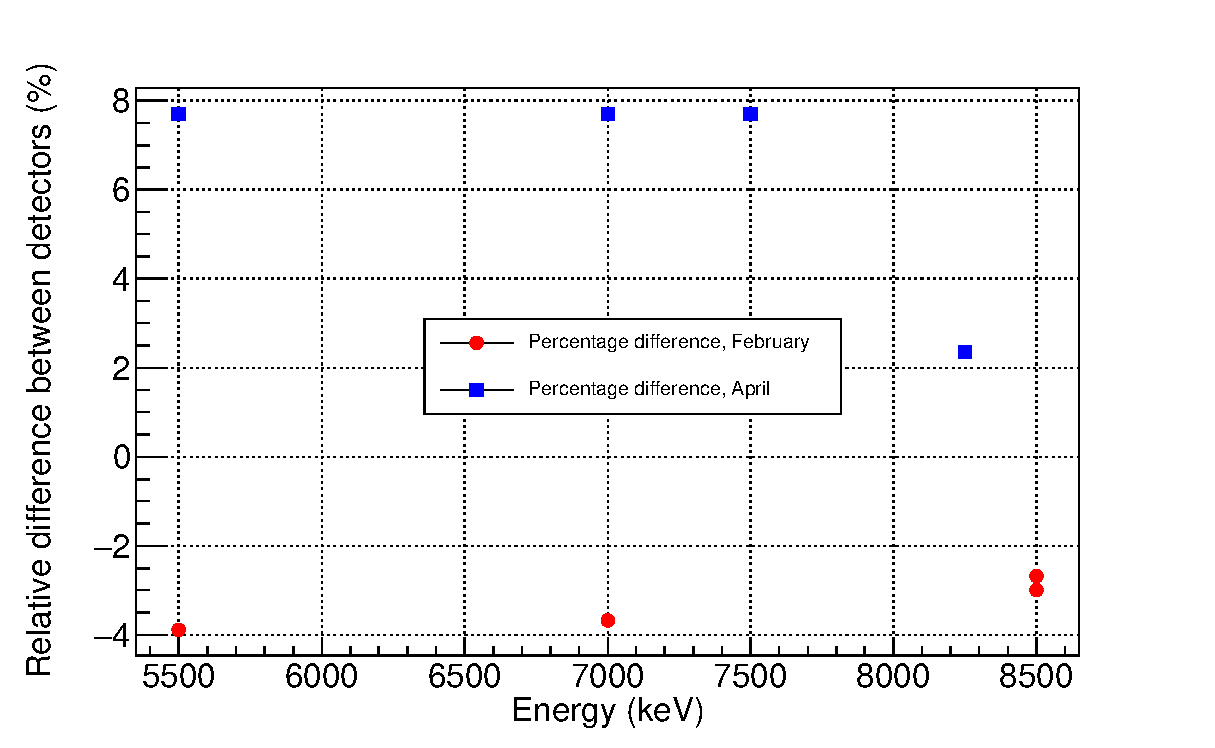
\includegraphics[width=0.80\textwidth]{decay_errors_rel_per_fixed.eps}
	\caption{Same as figure \ref{decay_errors_rel_per}, but without measurements 5 and 6.}
	\label{decay_errors_rel_per_fixed}
\end{figure}

The best agreements between detectors are for the measurements at higher energies, in both months.
The differences barely changing at energies under \qty{8}{\MeV}, and we can see at \qty{8.5}{\MeV}, where we have two measurements, that they give very similar numbers.
All of this tells us that this difference is due to a systemic error, and that it is likely dependent on the energy of the accelerator.

Regardless, agreement between detectors is good and consistent, and going forward we will represent, for each measurement and method, the average between both detectors.
Their error bars will be $\pm$ the relative differences calculated above.

\subsection{Agreement between fit methods}
To determine the agreement between the different fit methods, we can calculate the relative difference between the results given by each, with the same formula as in the previous point.
In figure \ref{activation_method_comparison} are represented the relative difference when comparing:
\begin{itemize}
	\item \textit{Unified} with \textit{rise}, drawn with crosses.
	\item \textit{Unified} with \textit{decay}, drawn with Xs.
	\item \textit{Decay} with the average between \textit{rise} and \textit{unified}, drawn with squares.
		This one is to compare the most conventional way of doing activation measurements with the more numerial method.
\end{itemize}
Because we have already discarded measurements 5 and 6 completely, and we don't have current data (and thus \textit{rise} and \textit{unified} results) for mesurements 4, 8, 9, and 10; we only have 4 measurements to do this comparison with.
Luckily, they are each at a different alpha energy.

\begin{figure}[H]
	\centering
	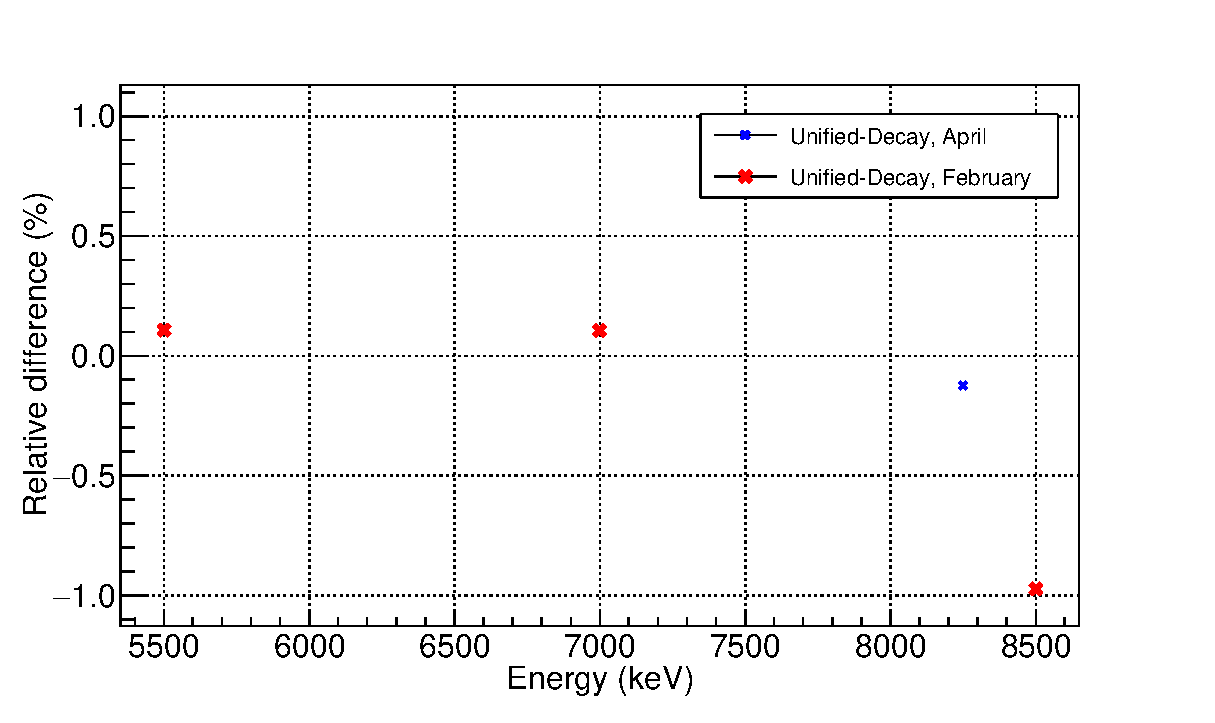
\includegraphics[width=0.80\textwidth]{activation_method_comparison.eps}
	\caption{Relative difference between the different fitting methods, with different symbols for each comparison; and color for each month.}
	\label{activation_method_comparison}
\end{figure}

We can see that the agreement is under \qty{9}{\percent} between \textit{unified} and \textit{rise}, and under \qty{1}{\percent} between \textit{unified} and \textit{decay}, for all measurements.
It seems from the results that the \textit{rise} method is the one in most disagreement with the others.
The difference between \textit{decay} and the average between \textit{unified} and \textit{rise} is thus mostly due to the \textit{rise} results being more discordant.

This disagreement with \textit{rise} seems to correlate with the current being less constant for measurements 1 and 3 (energies \num{5.5} and \num{8.5} in figure \ref{activation_method_comparison}) and, more noticeably, having abrupt changes compared to measurements 2 and 7.
More measurements are needed to make sure, but a sudden change in current mostly means a change in the \textit{extra background}.
It makes sense that the results are worse, as \textit{unified} is able to give a better fit for the proportionality constant that determines the \textit{extra background}, by virtue of also analyzing the sudden change at the beginning and end of activation.
\\

We will, then, discard the \textit{rise} results and use only the \textit{decay} results moving forward.
Representing the \textit{decay-unified} average would restrict us to only 4 measurements, so we will represent \textit{decay} results for all 8\footnote{Measurements 5 and 6 were removed.}, knowing they agree within \qty{1}{\percent}.

\subsection{Disagreement with EXFOR data}
When comparing the results we have obtained with EXFOR data, the disagreement is very large, around a factor of \num{1.9}.
In figure \ref{activation_final_results}, we plot the absolute results for the thick target yield, along with the raw data from EXFOR.
We also plot the EXFOR data scale up by \num{1.9}, to show that the results follow the same shape, but higher.

\begin{figure}[H]
	\centering
	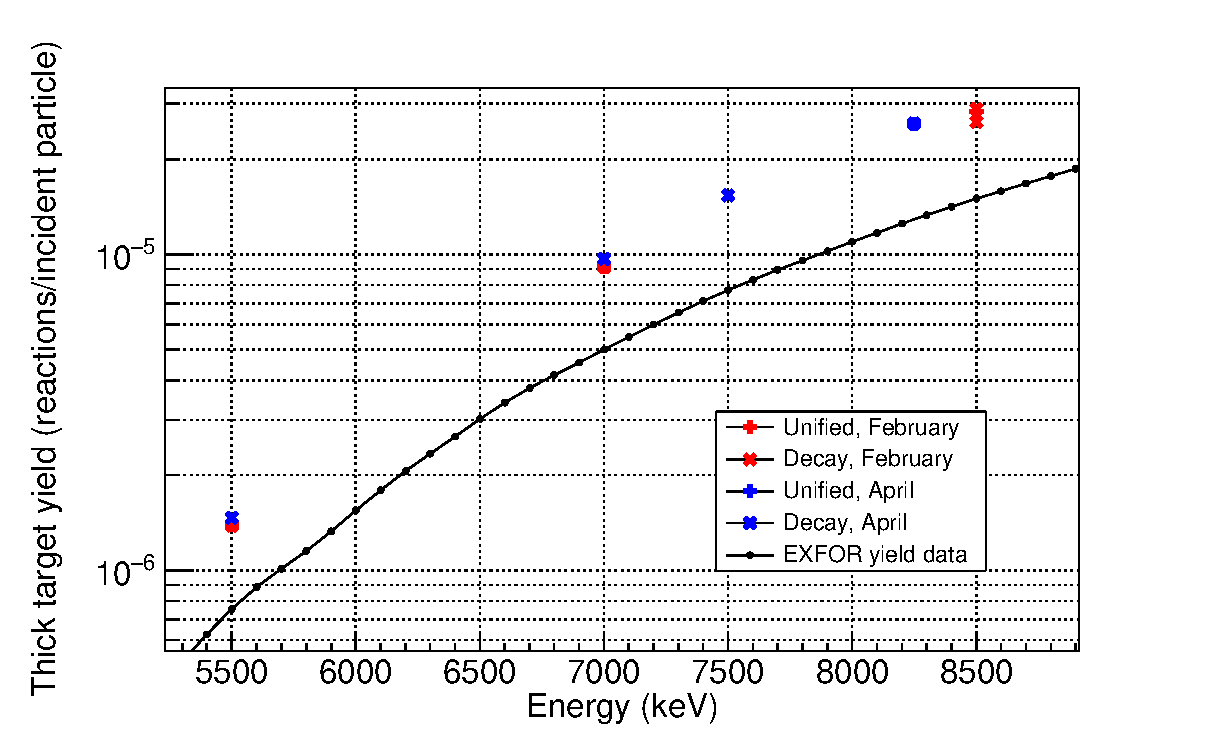
\includegraphics[width=0.80\textwidth]{activation_final_results.eps}
	\caption{Final results for thick target yield, next to the data from EXFOR and a scaled up version.}
	\label{activation_final_results}
\end{figure}

Figure \ref{activation_result_diffs} shows the ratio of results over EXFOR.

\begin{figure}[H]
	\centering
	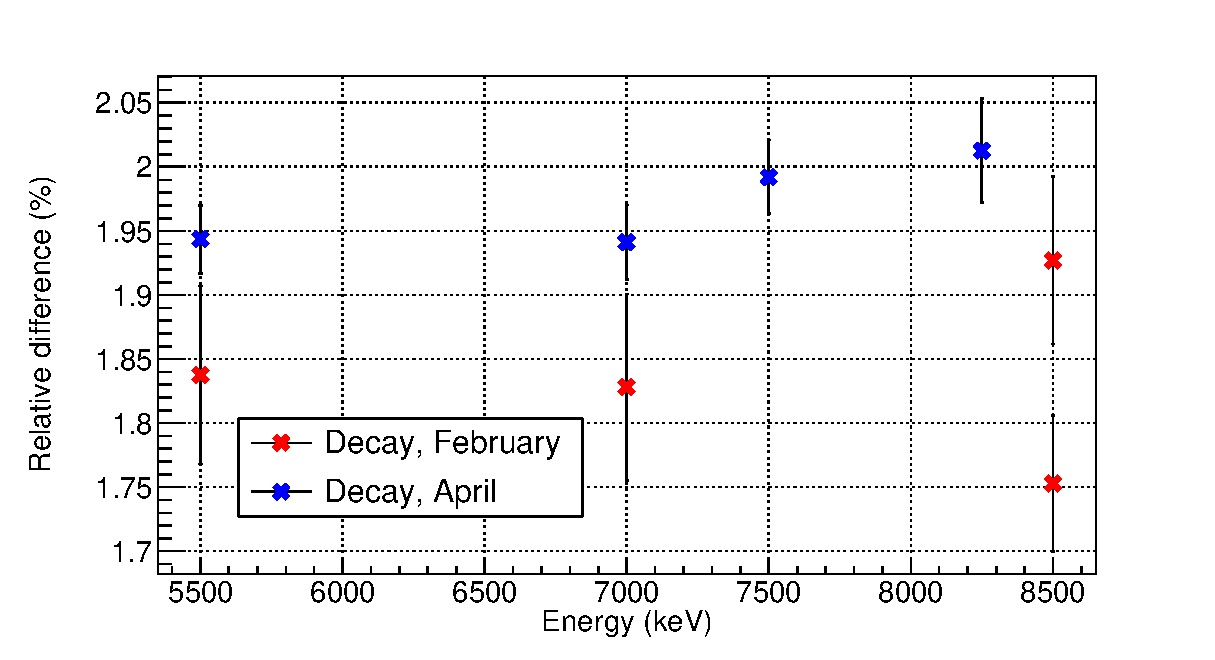
\includegraphics[width=0.80\textwidth]{activation_result_diffs.eps}
	\caption{Relative difference of different methods with respect to EXFOR data.
	\qty{+100}{\percent} difference means the result is double the expected.}
	\label{activation_result_diffs}
\end{figure}

We can see that the results are almost double the expected, and also that they deviate more for energies higher than \qty{7}{\MeV}; meaning their shape is also not completely the same (although the difference is small), the curve grows somewhat faster.
The lower point at \qty{8.5}{\MeV} corresponds to measurement 4, done on February but on the second day, unlike the others.
The difficulties with the Tandem at higher energies might explain the diverging results there.
For measurement 4 specifically, some other change from one day to the next might be a possible explanation for it decreasing instead of increasing, the same way measurements change from February to April.

We can compare the results by month and see that, for April, they are consistently higher than for February, but not by much.
For the two energies where we can compare \textit{decay} results, the difference is of \qty{2.8}{\percent} for \qty{5.5}{\MeV} and \qty{3.0}{\percent} for \qty{7.0}{\MeV} (compared to their average).
\\

In conclusion, although the activation measurements are consistent with each other and their shape is consistent with EXFOR; they are all too high, multiplied by a factor of around \num{1.9}.
This is most likely due to an unidentified error in the data analysis, whose cause remains a mistery.
Other possible causes, like errors in the measurement process, are not consistent with the results being in accord with each other so well.
The error must also, by necessity, affect all methods employed to arrive at the results equally; which remove the possiblity of it being specific to any one fitting method.

In the end, it could not be found.


%%%
%%%	TOF
%%%

\chapter{Measuring neutron energy by time-of-flight}

\section{The time-of-flight experiments}
The most accurate, and sometimes the only, method for determining the kinetic energy energy of a neutron is by time-of-flight.

\subsection{The time-of-flight principle} 
This method requires that the beam of particles producing the neutrons features a pulsed beam structure: the alphas should arrive in narrow pulses spaced with a certain period, producing as a results neutrons also in the form of pulses.
\\

The time that the radiation needs to reach the detector since it is produced is called the \textit{time-of-flight}, or ToF.
In the case of $\gamma$-rays, they move at the speed of light $c$, and thus all arrive at the detector at $\text{ToF}=L/c$, with $L$ the distance to the target, forming the so-called  \textit{gamma flash}.
Neutrons, however, have different speeds depending on their kinetic energy and therefore arrive at the detector with a ToF distribution from which the neutron energy distribution produced by the \an reaction can be extracted.
For each neutron:
\begin{equation}
	E_n=\frac{1}{2} m_n \left( \frac{L}{\text{ToF}} \right)^2 = \frac{1}{2} m_n \left( \frac{L}{t_n - t_{flash} + L/c} \right)^2
	\label{Eq_ToF2En}
\end{equation}
where $L$ is the distance between the target and the detector, and where the ToF of the neutrons is calculated in reference to the time of the $\gamma$-flash $t_{flash}$ and of the neutron $t_n$ in reference to some other point in time.

The neutron energy resolution that can be achieved can be calculated through propagation of errors as:
\begin{equation}
    \frac{\Delta E_n}{E_n} =
    \label{Eq_Enresolution}
\end{equation}

Hence, the resolution is better as the detector is placed further from the target and as the beam pulses become narrower (as this is it what causes  $\Delta$t$_{flash}$, the fact the alphas do not arrive all at the same time).
The beam pulses always have a certain width that generally can be approximated by a Gaussian distribution.

In order to study the time structure of the beam pulse, the shape of the observed $\gamma$-flash is a good proxy, because the photons travel all at the same speed and are directly caused by the alphas in the beam.
The gamma-flash will thus have the same shape as the alpha pulse, simply scaled by a factor and with an added background from other sources.

\subsection{Time-of-flight implementation at HISPANOS} 
In order to measure the ToF distribution, each time the accelerator's chopper acts, its internal clock emits an electric signal that is sent through a long cable to the DAQ, which takes it as a reference signal, from wich to determine $t_{flash}$ and $t_n$.
It doesn't correspond to when the pulse arrives at the target, as the time the particles take to cover the distance is not the same as the time taken by the electric signal to travel along the cable and be registered.

The detector signals from photons and neutrons are registered and marked with the timestamp relative to the chopper clock.
The result is a ToF distribution of signals that, in order to have physical meaning, need just to be shifted so that the $\gamma$-flash falls in the $\text{ToF}=L/c$ position.
\\

An example of the observed $\gamma$-flash is displayed in figure \ref{example_gflash}.	%YO ENSEñARÍA SOLO UNA PARA PODER DESCRIBIRLA BIEN, Y LUEGO TODAS EN LA SIGUIENTE SECCION PARA DISCUTIR LA CASUÍSTICA
The time structure of the $\gamma$-flash is far from the ideal Dirac delta function.
First, it features a quasi-Gaussian profile with a FWHM of \qty{1.5}{\nano\second}, which will certainly affect the neutron energy resolution (see equation \ref{Eq_Enresolution}).
Then, it also features a tail with a bump at longer ToF values, and a constant background.
This is related to the fact that the buncher is optimized for protons and deuterons, but not for alpha particles.

In the worst case (measurement 1), the tail contains up to \qty{30}{\percent} of the overall $\gamma$-flash, which means that the time of arrival of the alpha beam is not very well determined.
Because of all this, we cannot really treat the $\gamma$-flashes as simple Gaussians when considering their effect in the neutron energy and its resolution.

\begin{figure}[H]
	\centering
	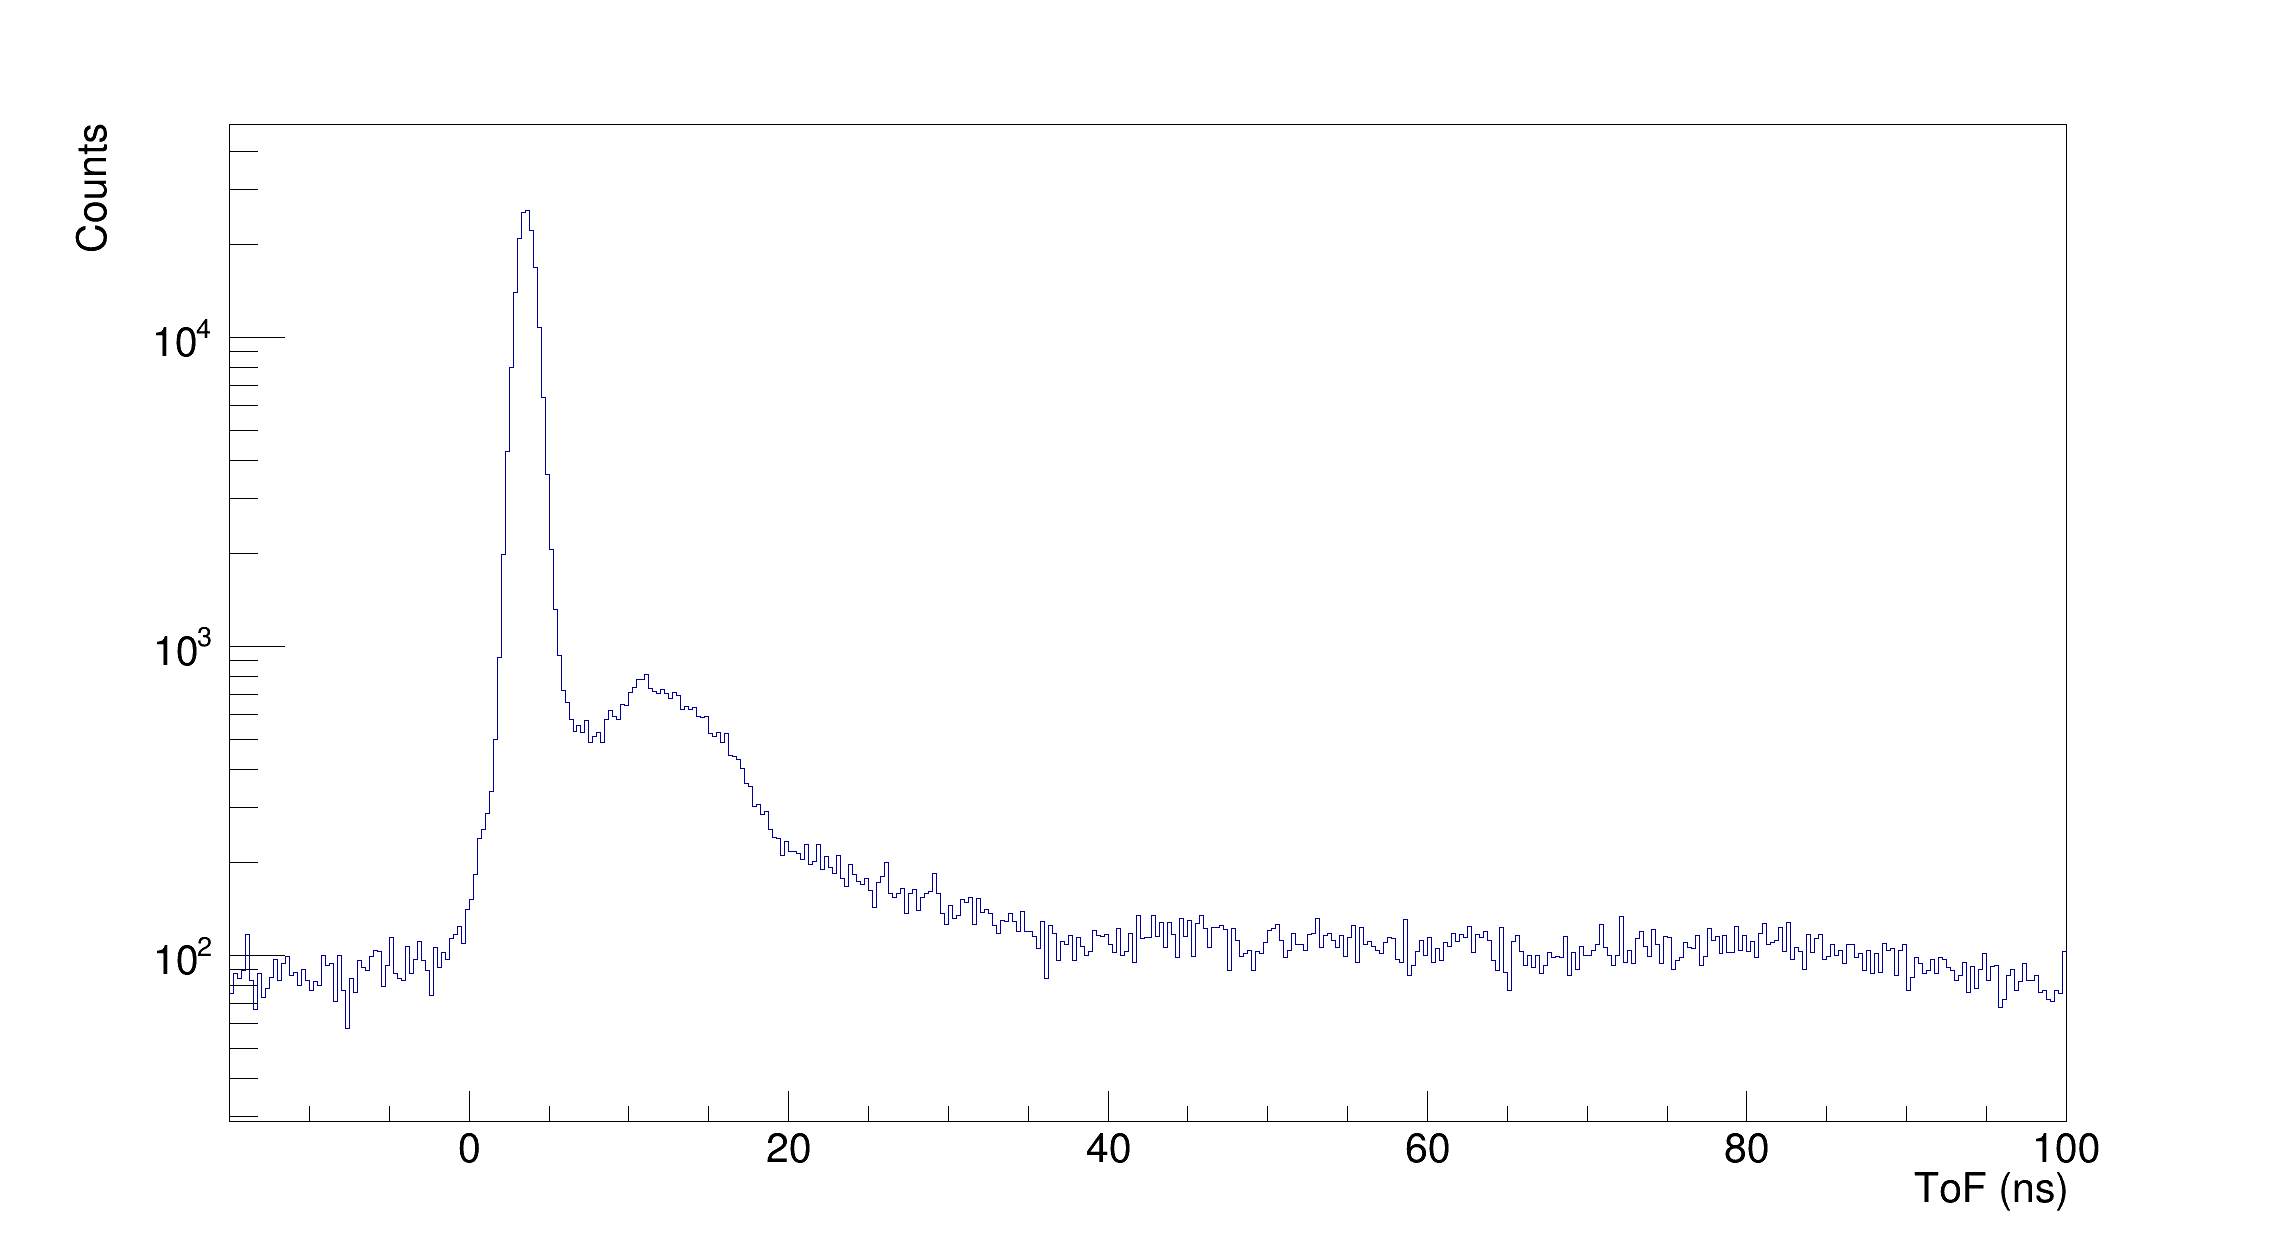
\includegraphics[width=0.80\textwidth]{example_gflash.png}
	\caption{Gamma flash of measurement number 3, in semi-logarithmic scale.}
	\label{example_gflash}
\end{figure}

\subsection{Measurements} 
The time-of-flight measurements carried out to study the \Aliso \an reaction took place on April 17th and 18th.
The details of the dates, beam energies, flight path distances and accumulated beam (charge) on target of each experiment are listed in Table \ref{pulsed_measurements_table}.

\begin{table}[H]	%Tabla con datos de las medidas de haz pulsado
\centering
\begin{tabular}[c]{>{\bfseries}r||c|c|c|c}
	N& Energy (\unit{\keV}) & Distance (\unit{\cm}) & Charge (\unit{\micro\coulomb}) & Date\tablefootnote{All took place in 2023} \\ \hline	%TBD?incertidumbre en distancia?
	1&\num{5500}&\num{100.0(25)}&?? &April 17\textsuperscript{th}\\ \hline
	2&\num{5500}&\num{100.0(25)}&?? &April 18\textsuperscript{th}\\ \hline
	3&\num{7000}&\num{100.0(25)}&?? &April 18\textsuperscript{th}\\ \hline
	4&\num{8250}&\num{100.0(25)}&?? &April 18\textsuperscript{th}\\ \hline
	5&\num{8250}&\num{200.0(25)}&?? &April 18\textsuperscript{th}\\ \hline
\end{tabular}
\caption{Summary of the time-of-flight experiments carried out.}
\label{pulsed_measurements_table}
\end{table}

The single measurement on the 17th was a test and had a very low current, featuring also the highest tail in its $\gamma$-flash (\qty{30}{\percent} of counts), thus it was discarded in the analysis.
On the other hand, the experiments with the maximum beam energy was repeated at two different distances, in order to assess the expected improvement in neutron energy resolution.

\begin{figure}[H]
	\centering
	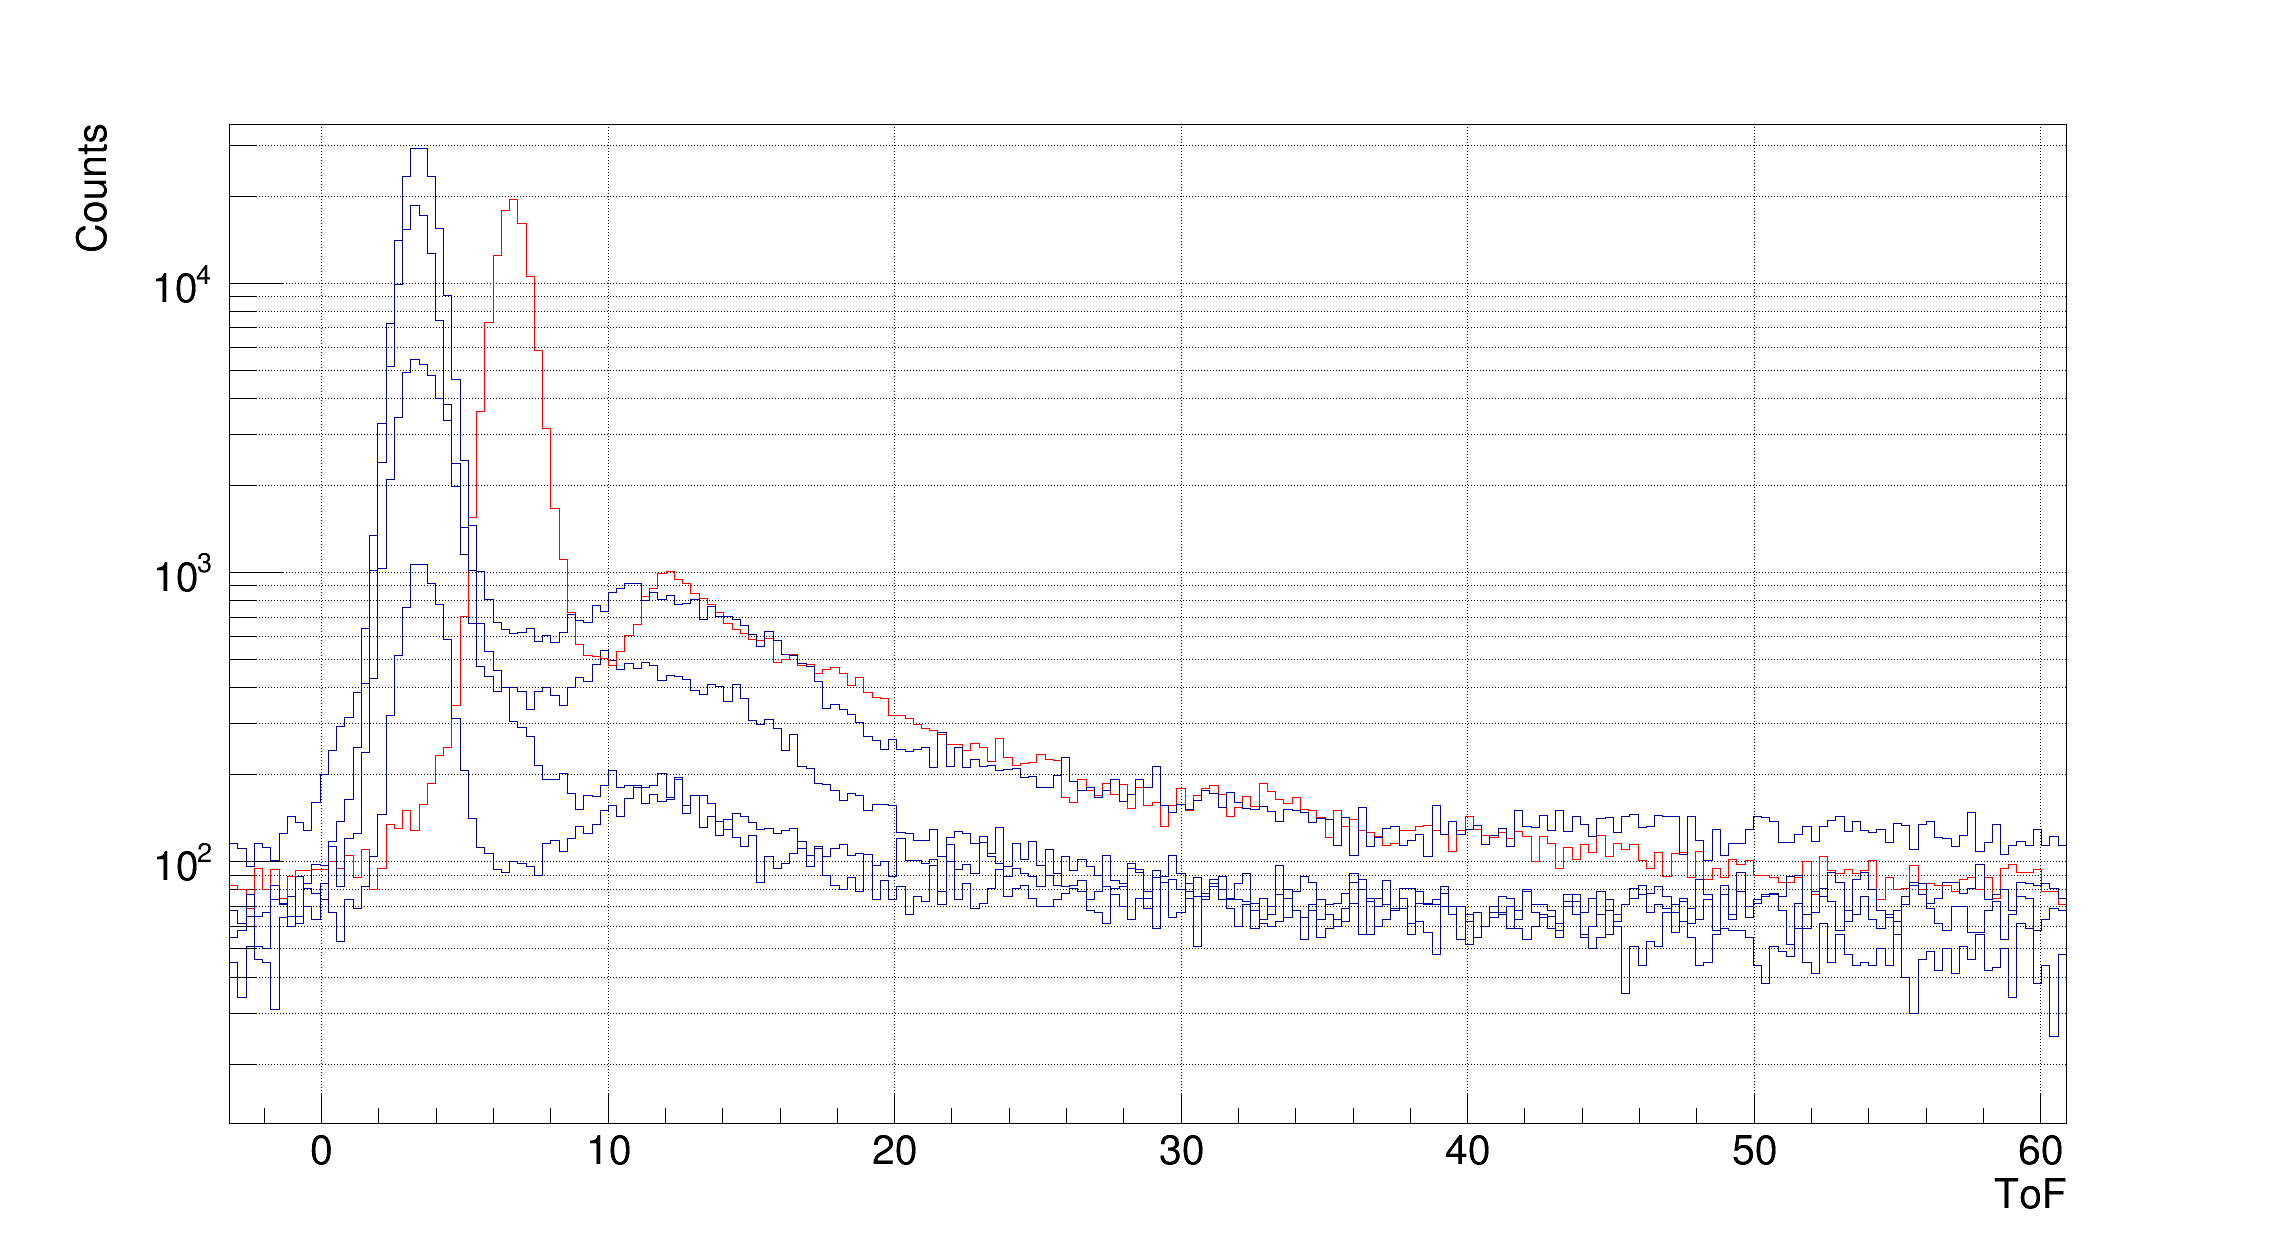
\includegraphics[width=0.80\textwidth]{uneven_gflash.png}
	\caption{Superposition of all histograms of gamma flashes.
	In red is a measurement taken at double the distance than the others.
	It is displaced to the right because of the longer time photons take to travel the distance to the detector.
	Their shape will be that of their corresponding alpha pulses, plus a background.}
	\label{uneven_gflash}
\end{figure}

\section{Data analysis}
The objective of our analysis is to obtain the energy spectra of the neutrons generated by the \an reactions.
To that end, we must first separate the gammas from the neutrons by using PSD, by using a figure such as \ref{example_psd}.
We thus get the gamma flash and the neutron response for each measurement.

\begin{figure}[H]
	\centering
	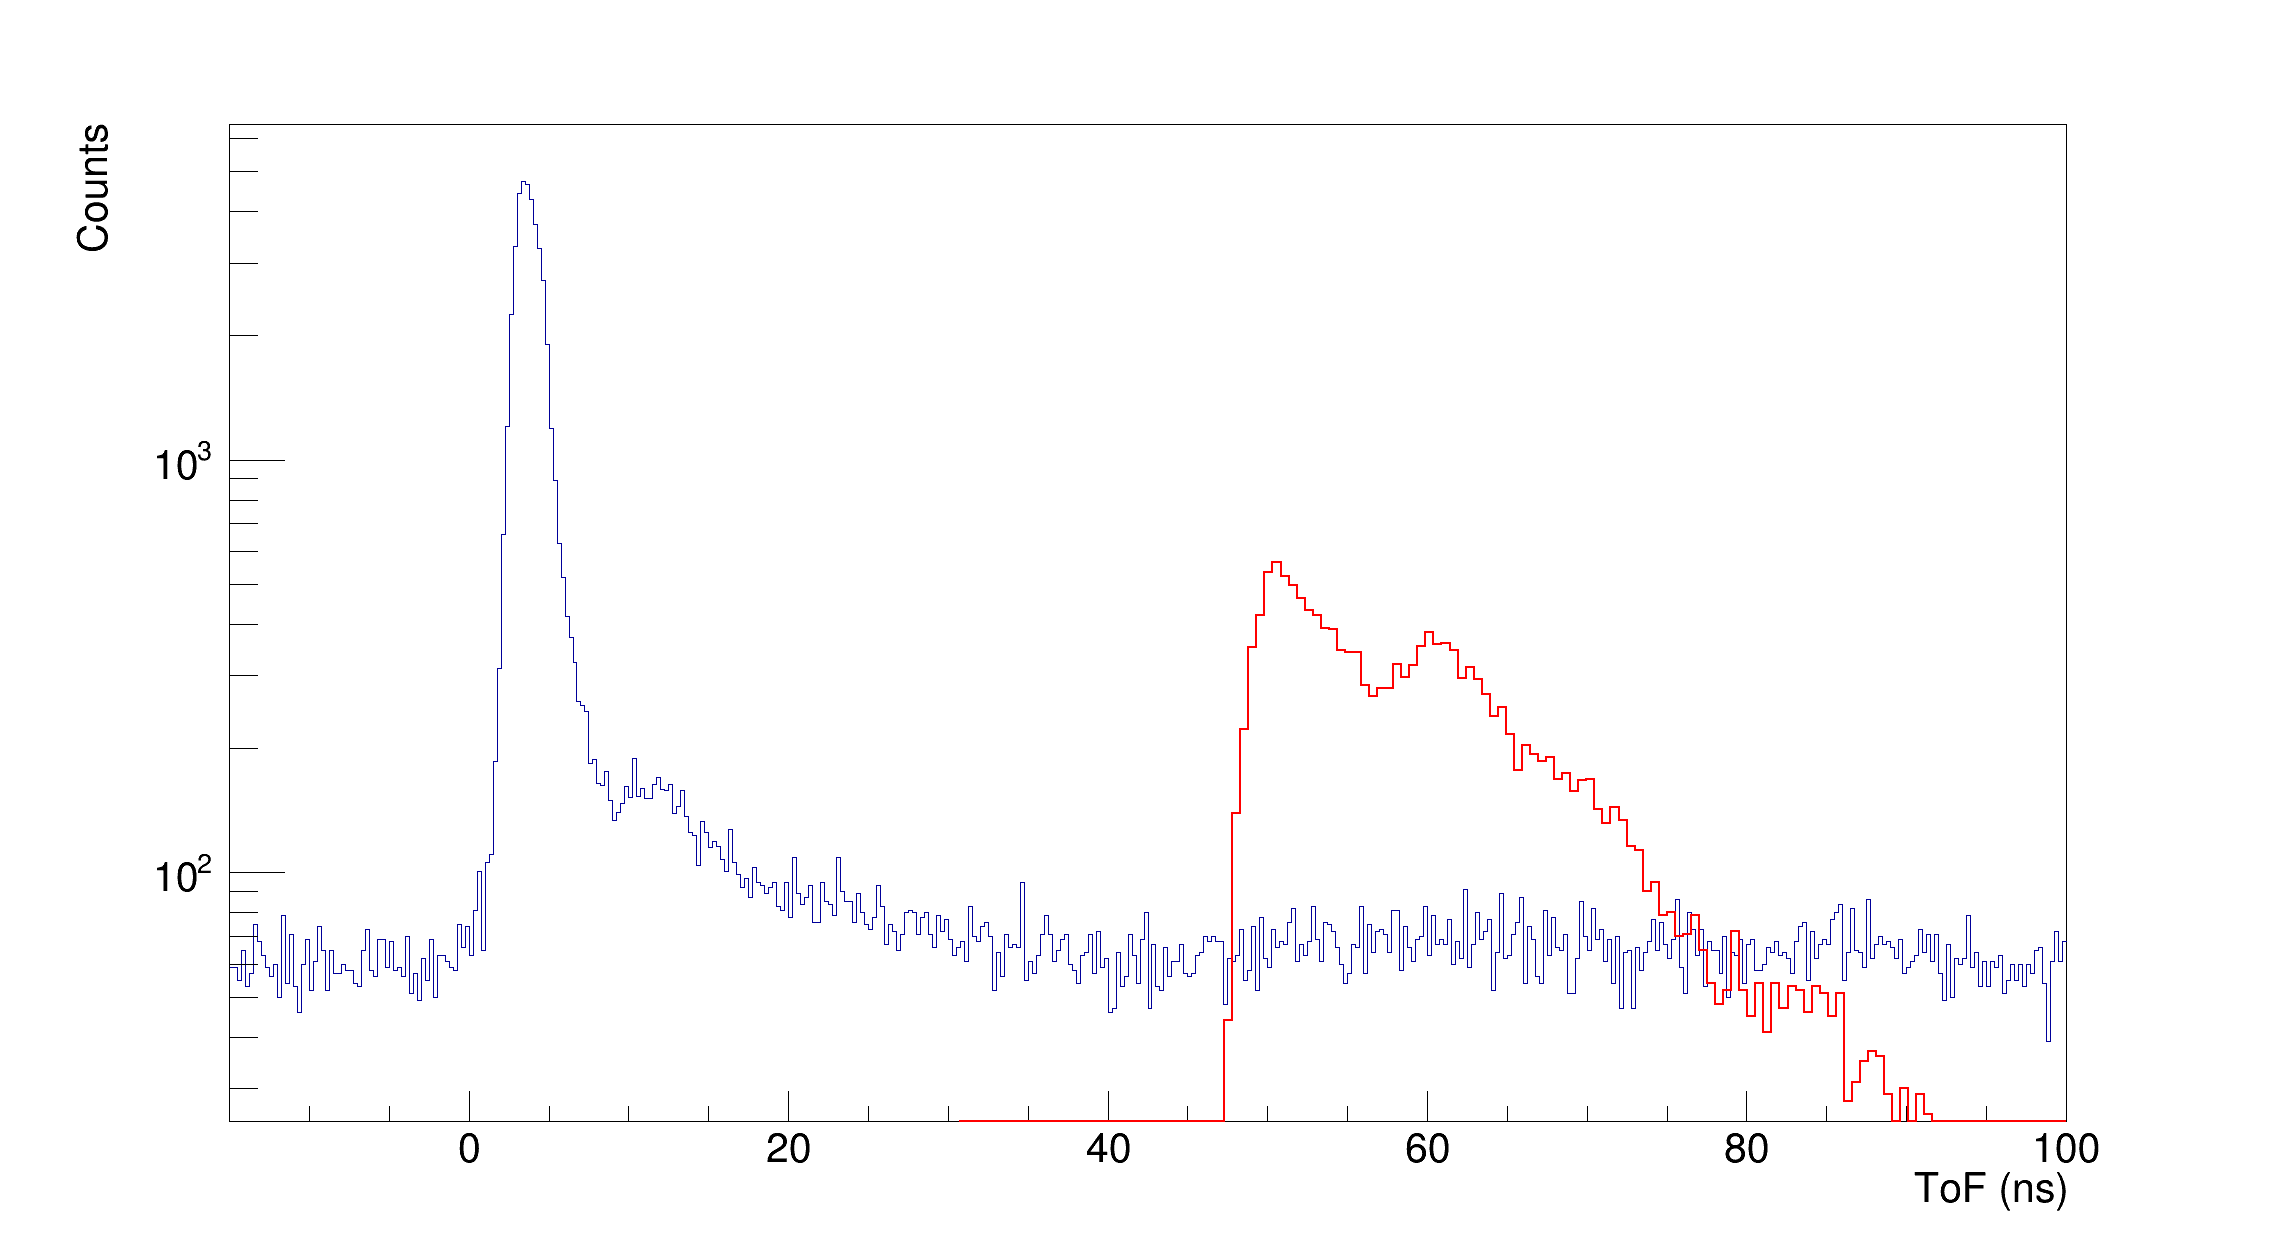
\includegraphics[width=0.80\textwidth]{separated_tof.png}
	\caption{Gamma flash (blue) and neutron response (red) for measurement number 2.}
	\label{separated_tof}
\end{figure}

To get the neutron energy spectra, we use two different methods of analysing the resulting gamma flash and neutron response for each measurement.

\subsection{Simple method}
This method makes use mostly of the neutron response counts.
We use the gamma flash histogram exclusively to get its center, by taking as the centroid when fitting it to a gaussian.
We then calculate the ToF of each neutron as:
\begin{equation}
	\text{ToF} = t_n-t_\text{flash}+\frac{L}{c}
\end{equation}
with $t_n$ the timestamp (with respect to the signal from the chopper) of the neutron, $t_\text{flash}$ the center of the gamma flash, and $L/c$ the time it takes the gammas to get to the detector, i.e., the ToF of the gamma flash.
From each time-of-flight, we can then get the energy of the neutron as:
\begin{equation}
	E=\frac{1}{2} m_\text{n} \left( \frac{d}{\text{ToF}} \right)^2
\end{equation}
with $m_\text{n}$ the mass of the neutron.

Representing the calculated energy of every count in the neutron response in a histogram, we get the energy spectrum of the detected neutrons.
We correct it by dividing every bin by the geometric efficiency of the detector and by its efficiency in energy (given by figure \ref{monster_efficiency}).

After dividing by the number of alphas and the width of the bins, the resulting plot (figure \ref{pulsed_energysimple}) is the energy spectrum of the neutrons produced in the \an reactions.

\begin{figure}[H]
	\centering
	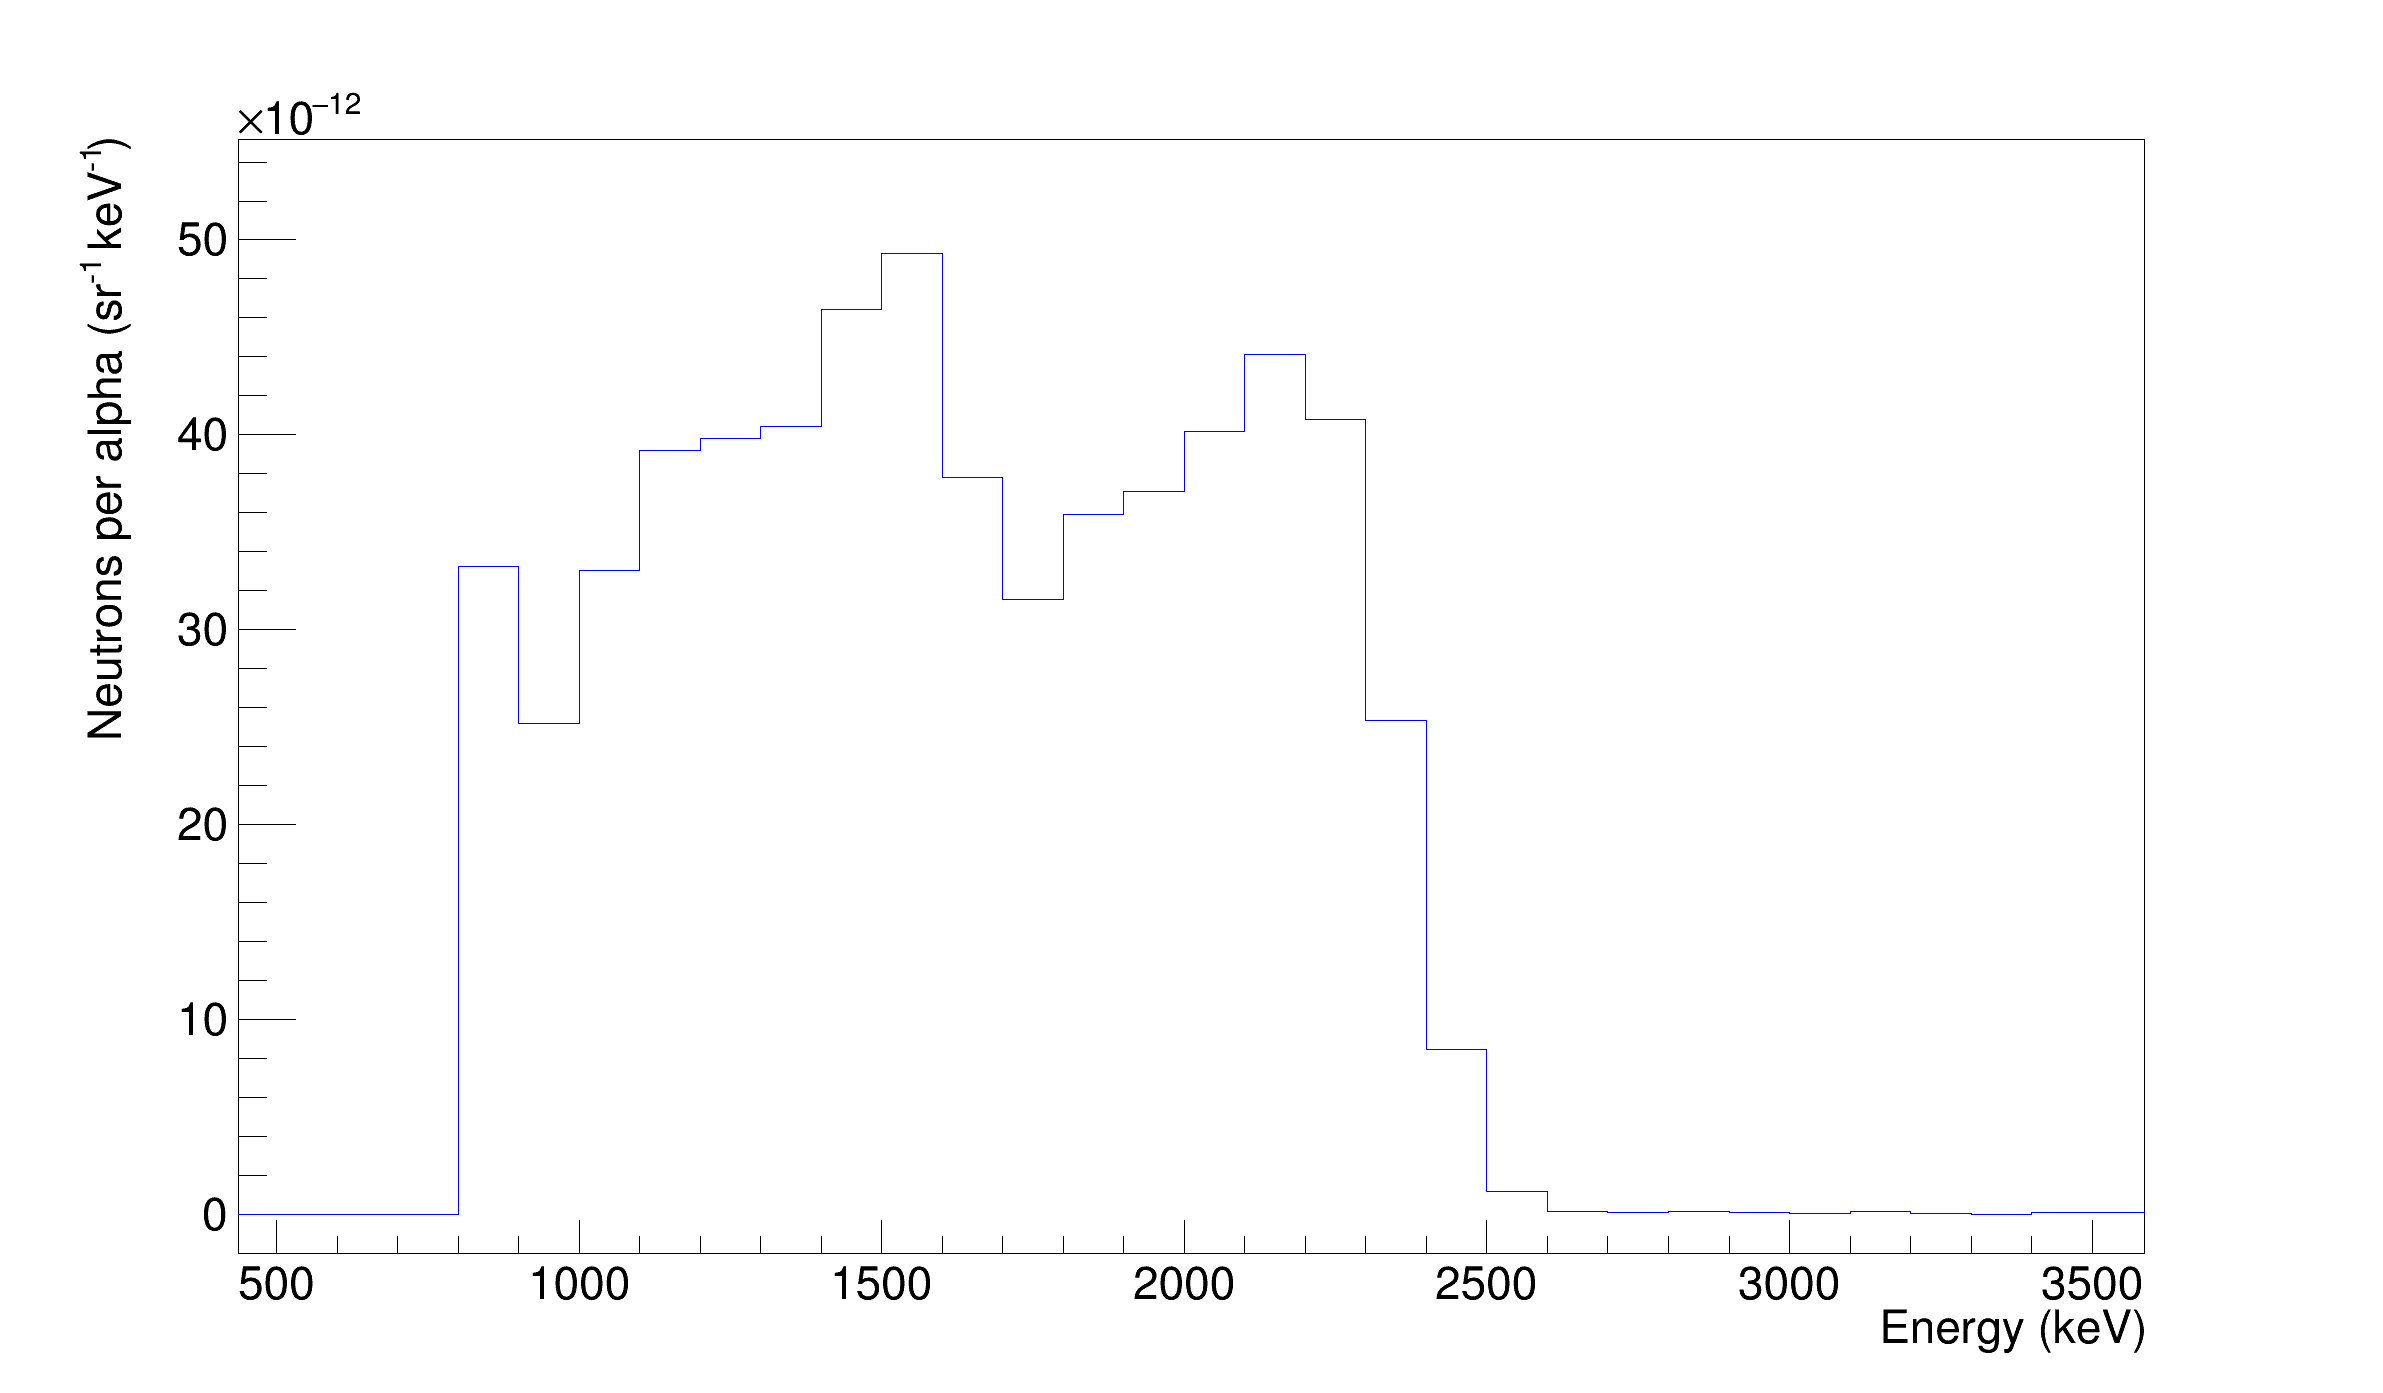
\includegraphics[width=0.80\textwidth]{pulsed_energysimple.png}
	\caption{Resulting energy spectrum for measurement number 2 using the simple method.}
	\label{pulsed_energysimple}
\end{figure}

This method doesn't consider the shape of the alpha pulse, rather it assumes all of the neutrons are created at the same time, $d/c$ time before the center of the gamma flash.
Also, an excess of neutrons with very long ToF, that bounce off the walls and take a longer path, are detected.
For the results (like figure \ref{pulsed_energysimple}), we simply remove all counts for which efficiency would be under \qty{15}{\percent}.

\subsection{Deconvolution}
We can take the shape of the alpha pulse into account by doing a deconvolution.
In order to do so, we fit the neutron response ToF histogram to a function that takes the gamma flash histogram as an input.

The function holds 50 parameters to be adjusted by the fitting, each associated with a certain time-of-flight.
Their values correspond to the number of neutrons of a certain ToF produced per gamma ray detected in the gamma flash.
The gamma flash is proportional to the alpha pulse, and so if we multiply the parameters by the total number of gammas in the gamma flash, and divide by the number of incident alphas, they get units of number of neutrons per incident alpha:
\begin{equation}
	\frac{\text{number of neutrons}}{\text{number of gammas}}\cdot \frac{\text{number of gammas}}{\text{number of alphas}} = \frac{\text{number of neutrons}}{\text{number of alphas}}
\end{equation}

Together, they form the neutron energy spectrum of the reaction, but in time-of-flight.
That is, the neutron response that would be generated by all of the alphas arriving at the same time, over the total number of alphas.

The result is to remove the effect of the width and assymetry of the gamma flash.
\\

The function goes through every bin in the gamma flash histogram, and scales that neutron response by the number of counts in it.
It adds together the contribution of all bins, and the result is, if the parameters are right, the measured neutron response.

In order to determine the parameters, ROOT: runs the function, compares the result with the measurements, adjusts the parameters, then repeats.

\begin{figure}[H]
	\centering
	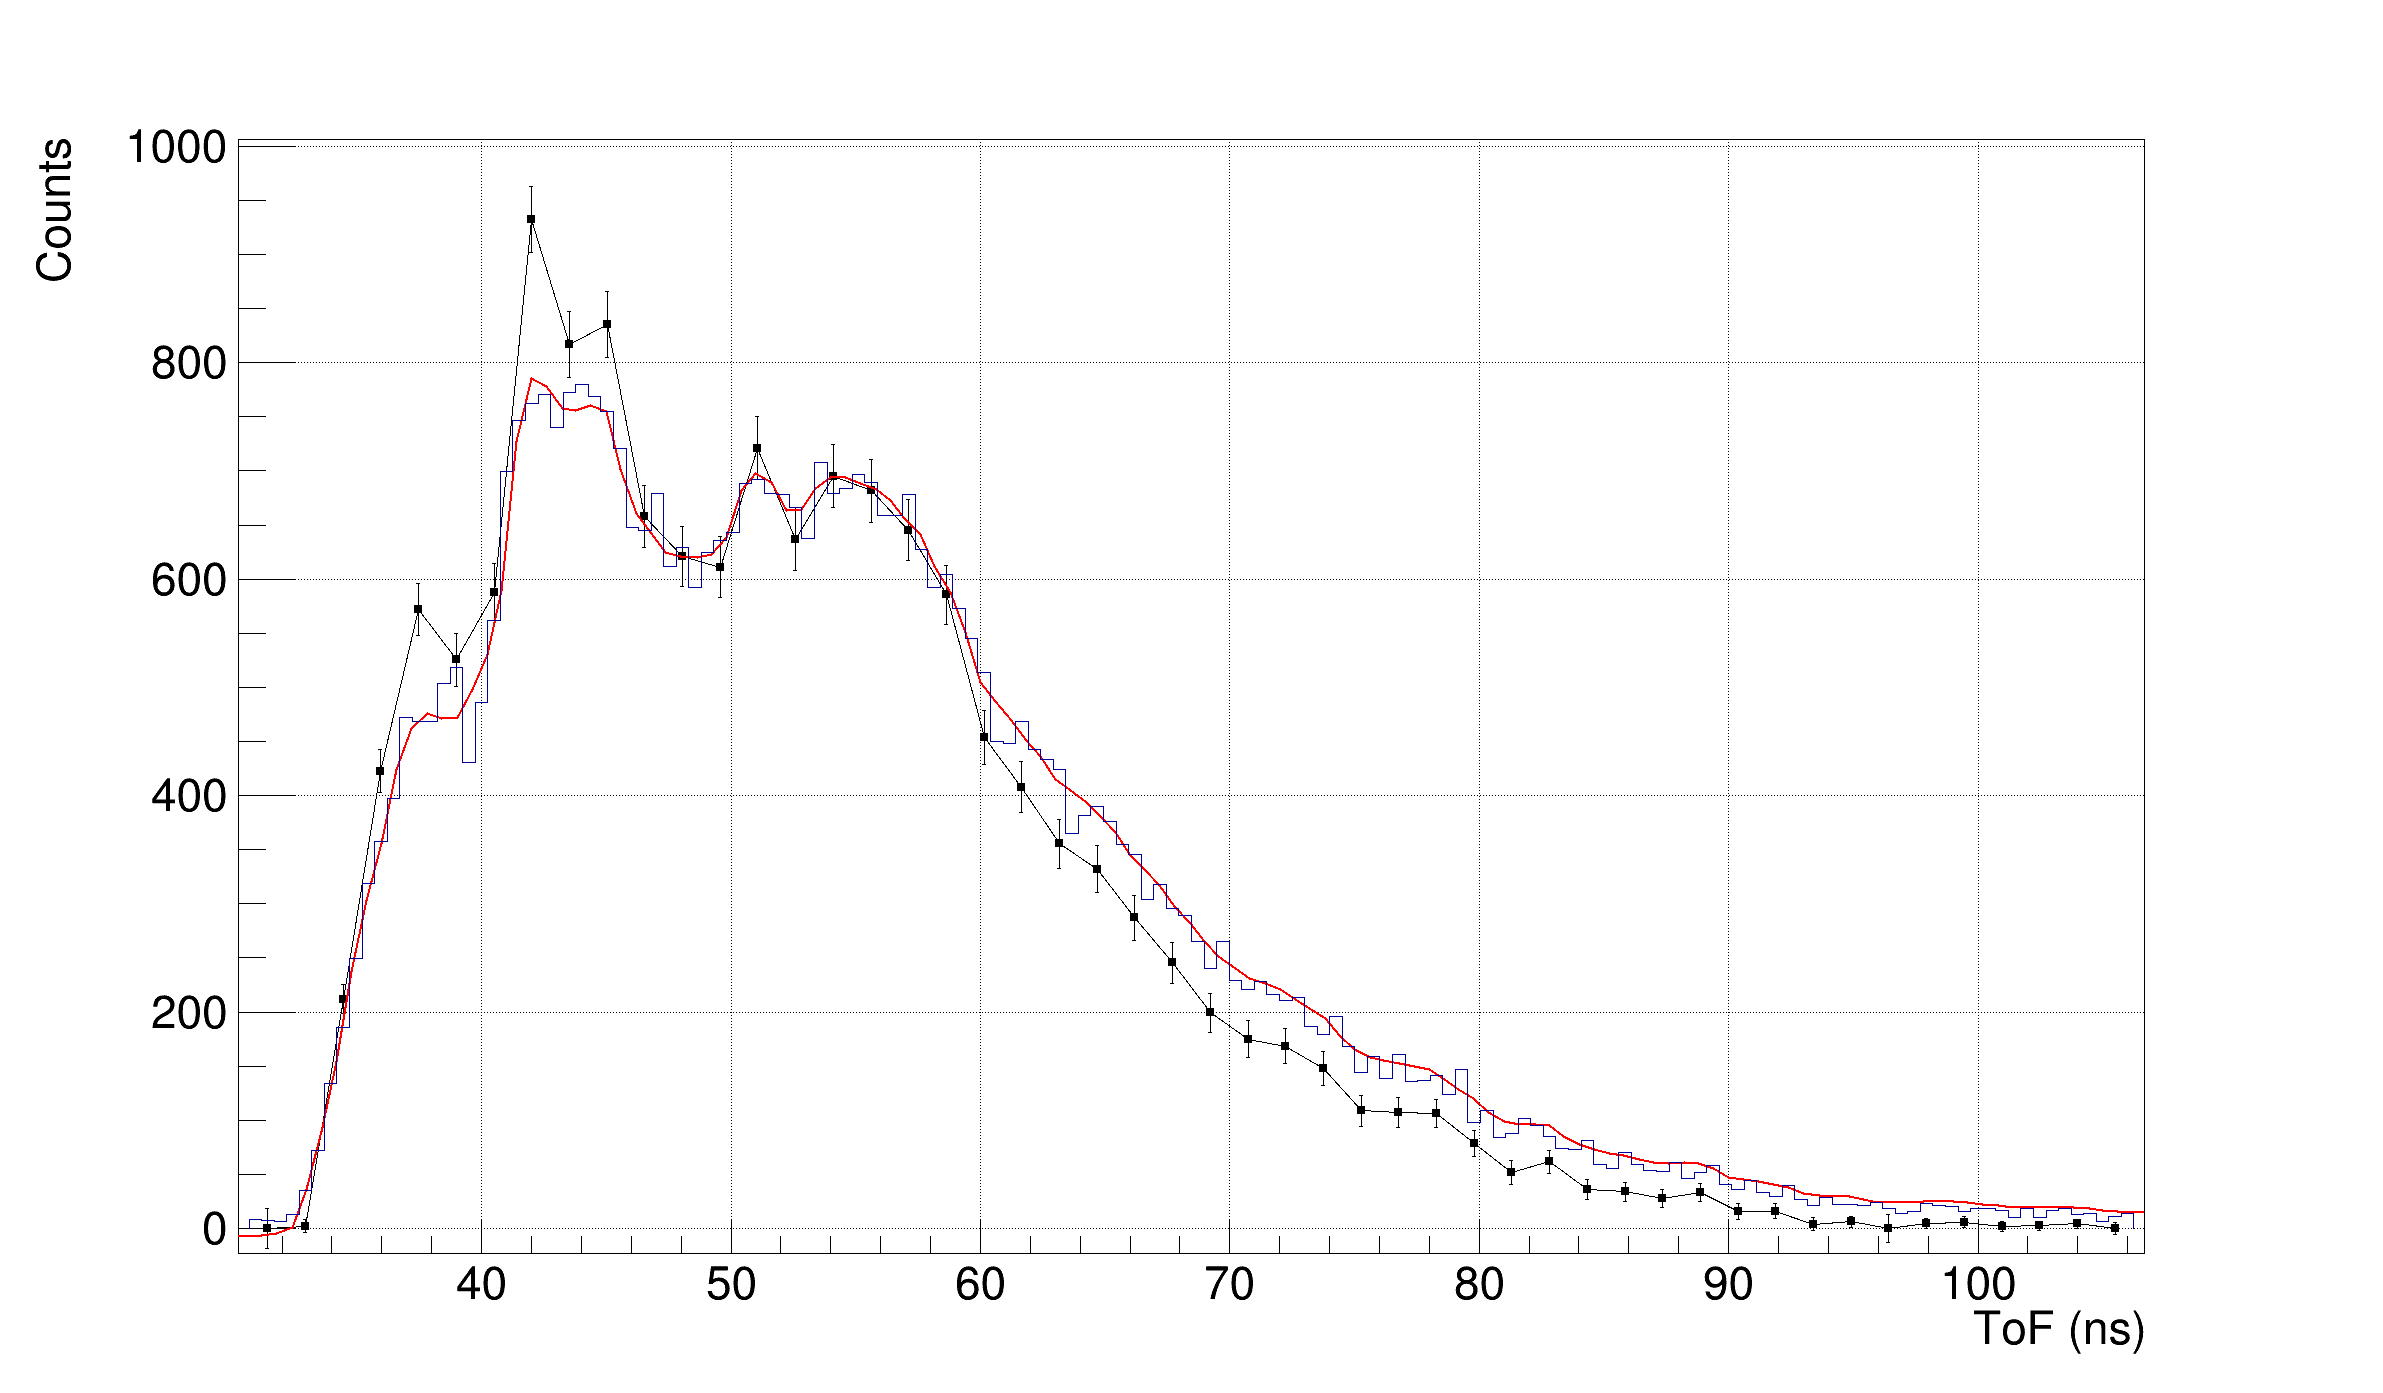
\includegraphics[width=0.80\textwidth]{pulsed_deconvolution_delta.png}
	\caption{Measured neutron response histogram (blue), result of the fitted deconvolution function (red) and parameters (black) for measurement number 4.}
	\label{pulsed_deconvolution_delta}
\end{figure}

\begin{figure}[H]
	\centering
	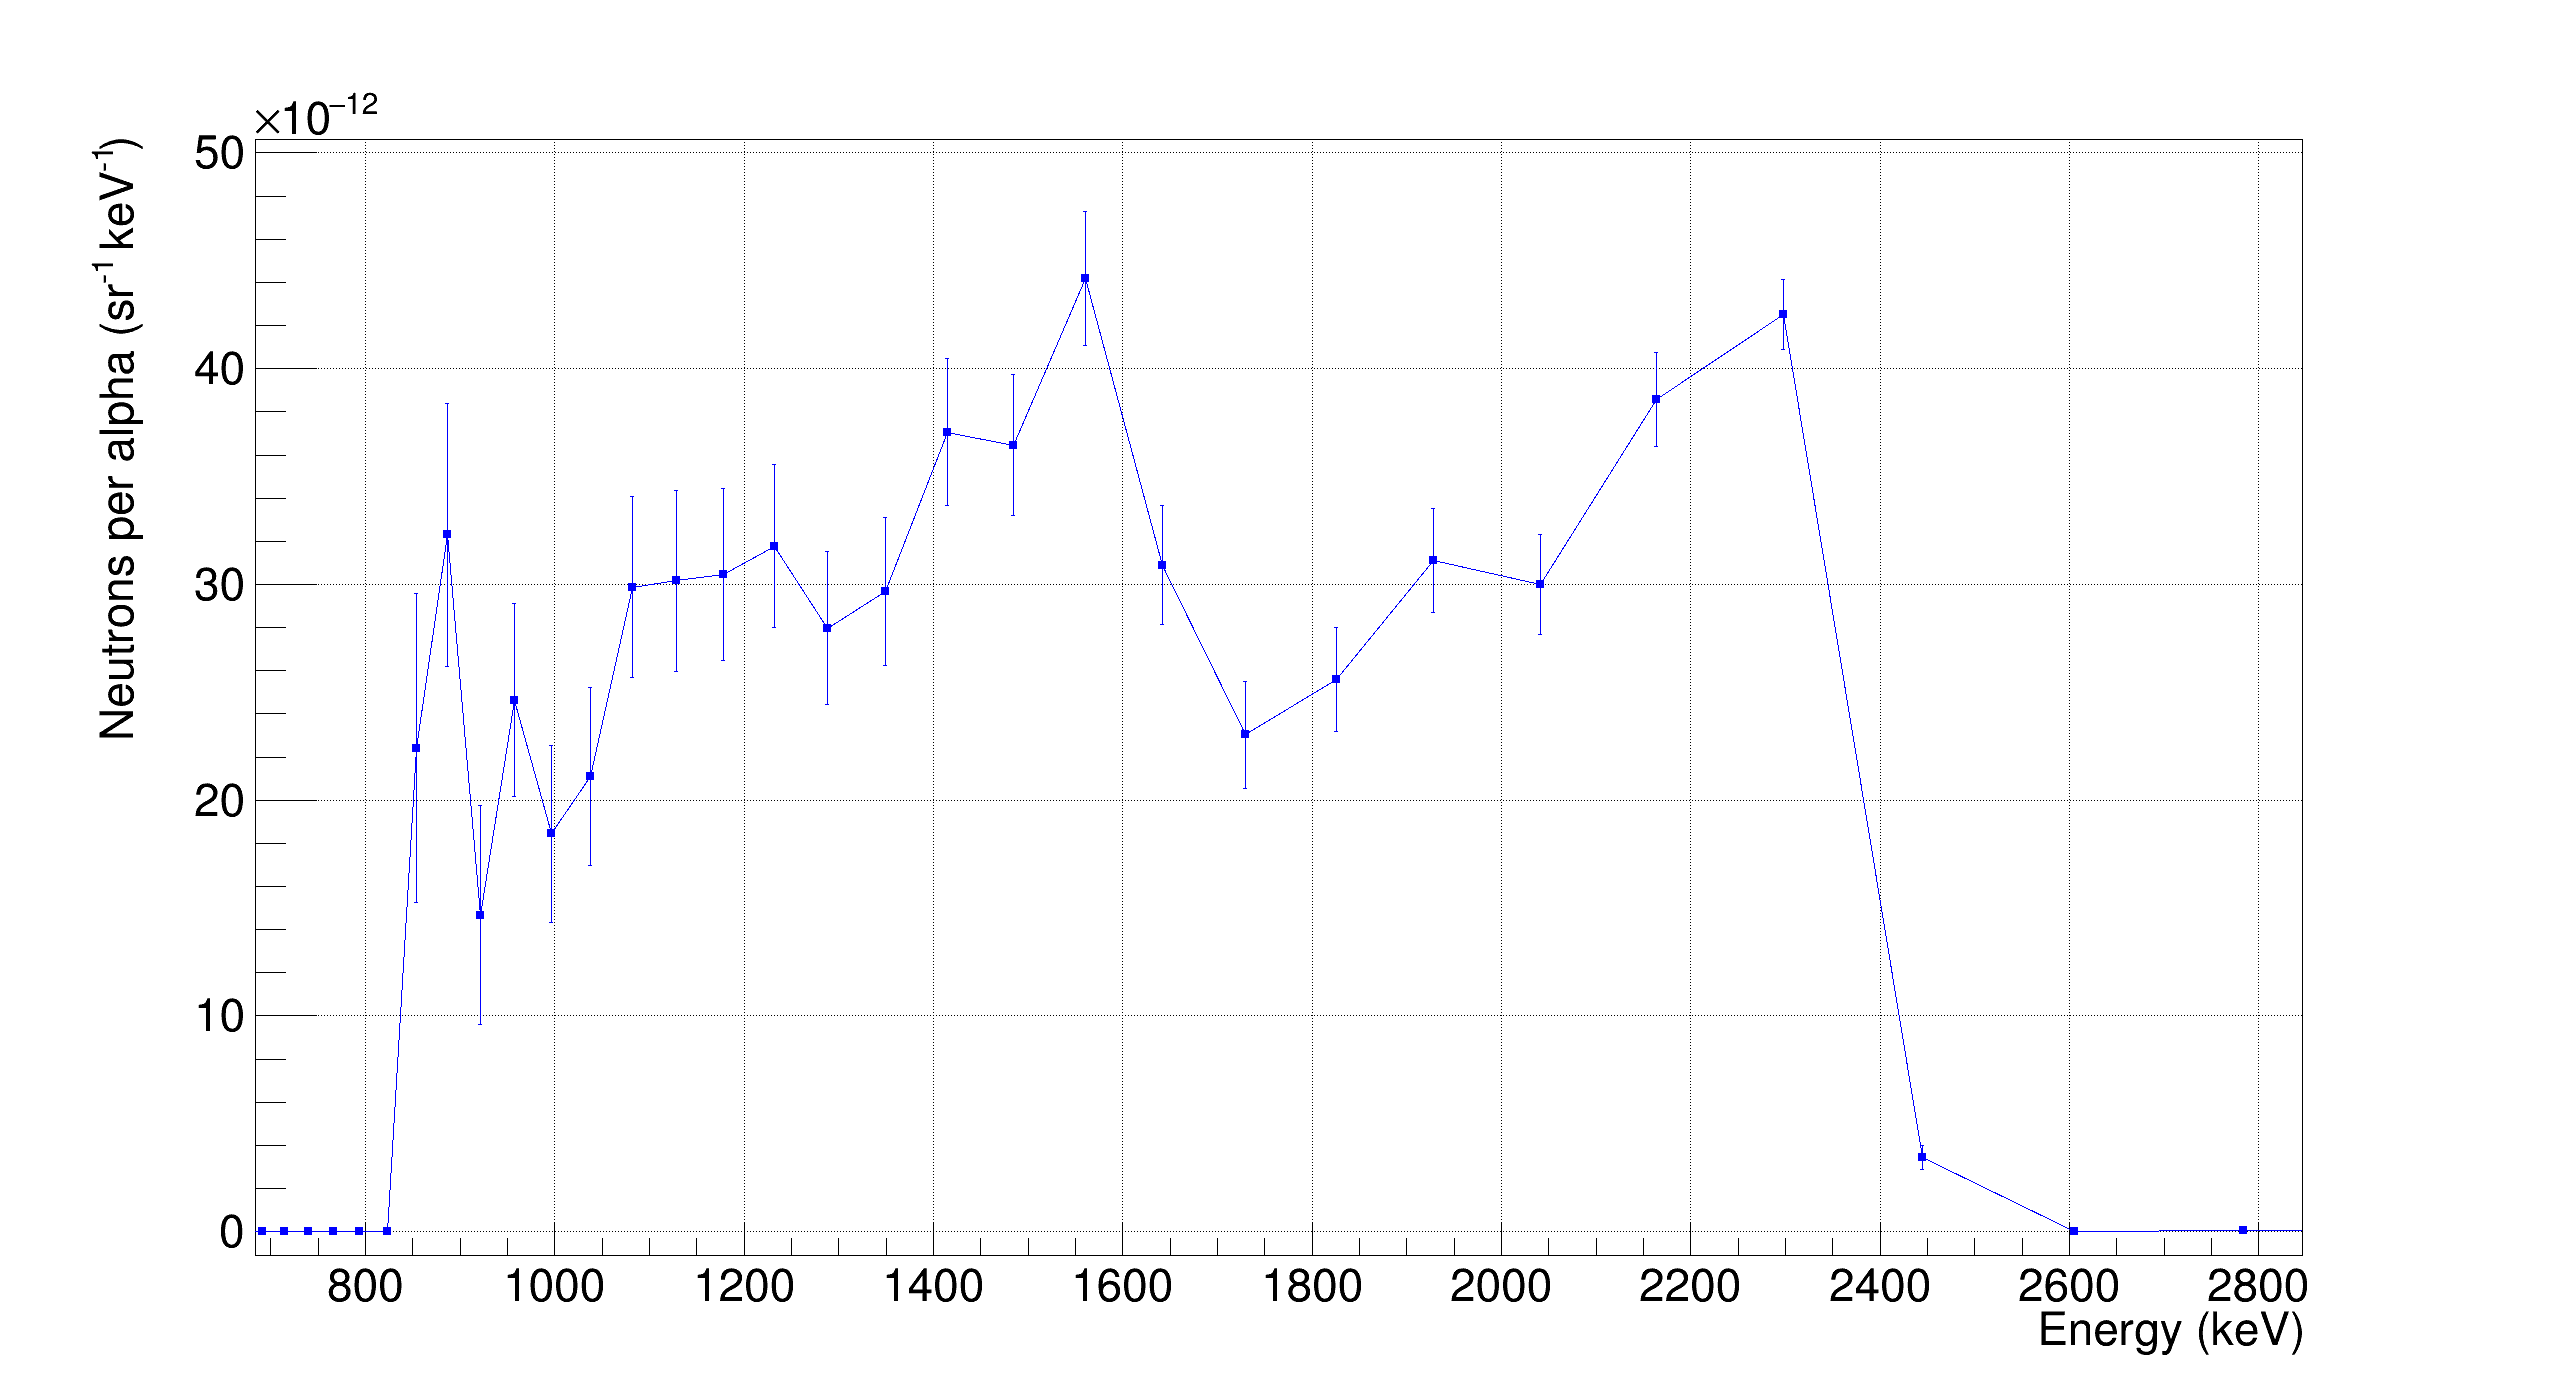
\includegraphics[width=0.80\textwidth]{pulsed_deconvolution.png}
	\caption{Parameters resulting from the deconvolution, forming the energy spectrum for measurement number 2.}
	\label{pulsed_deconvolution}
\end{figure}

\section{Results}
Both the simple method and the deconvolution agree with each other:
\begin{itemize}
	\item The deconvolution effectively moves some of the lower energy counts in the simple method spectra to higher energies, as they were created in the tail of the alpha pulses.
		Because of this, the deconvolution spectra are lower than the simple method's for low energies, and higher for higher energies.
	\item The deconvolution seems to only sometimes achieve better definition, which can be seen in the sharper peaks in the spectra.
		This is could in theory be improved with more parameters, but we run into problems with computing time and overfitting to noise.
\end{itemize}

Data to compare to only exists for the \qty{5.5}{\MeV} thick target yield spectrum.
We can see that the deconvolution matches quite well, while the simple method overestimates it, specially for low energies (figure \ref{pulsed_5mev}).
This is expected, because of the simple method taking neutrons with longer trajectories as having lower energies.

\begin{figure}[H]
	\centering
	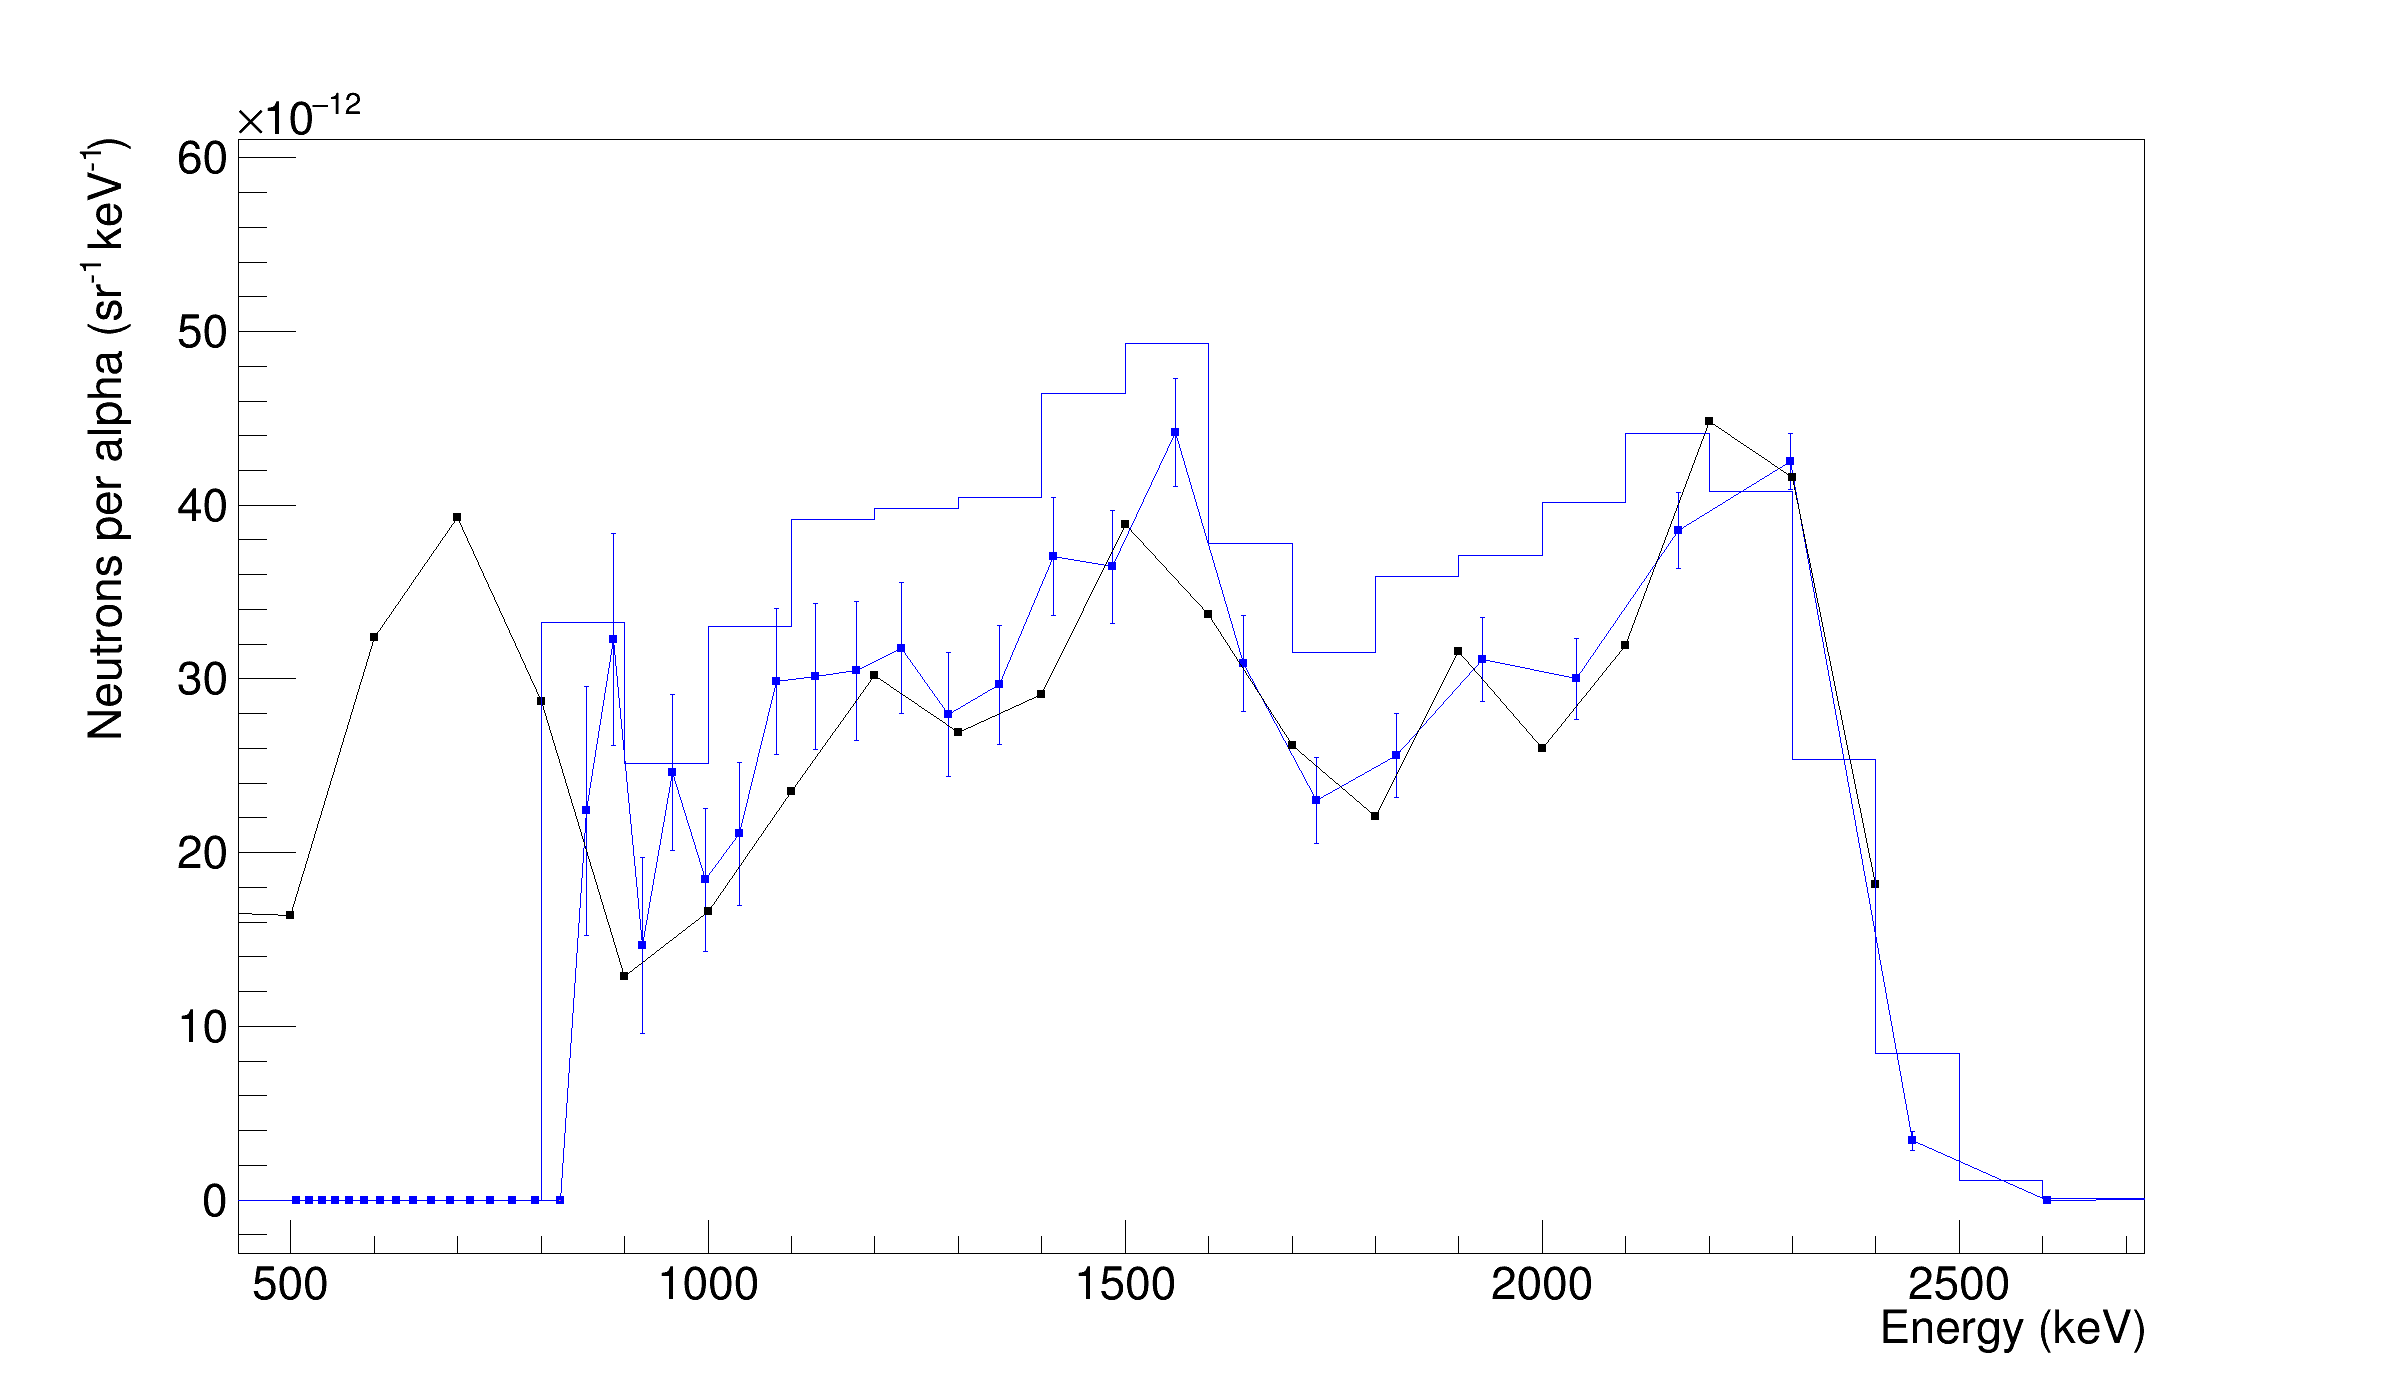
\includegraphics[width=0.80\textwidth]{pulsed_5mev.png}
	\caption{Neutron spectra for \qty{5500}{\keV}.
	EXFOR data (black), simple method (blue histogram) and deconvolution (blue squares).}
	\label{pulsed_5mev}
\end{figure}

For higher energies, there is no data to compare to.
However, we can calculate the maximum possible energy for neutrons, given the Q of the reaction and the cinematics; and see that that energy is not surpassed.
At \qty{8.5}{\MeV}, we also measured the spectrum at two different distances, and got similar results.

In general however, it is hard to estimate the uncertainty in deconvolution.
The error bars shown in the figures are the ones automatically calculated by the ROOT fitting method.

\begin{figure}[H]
	\centering
	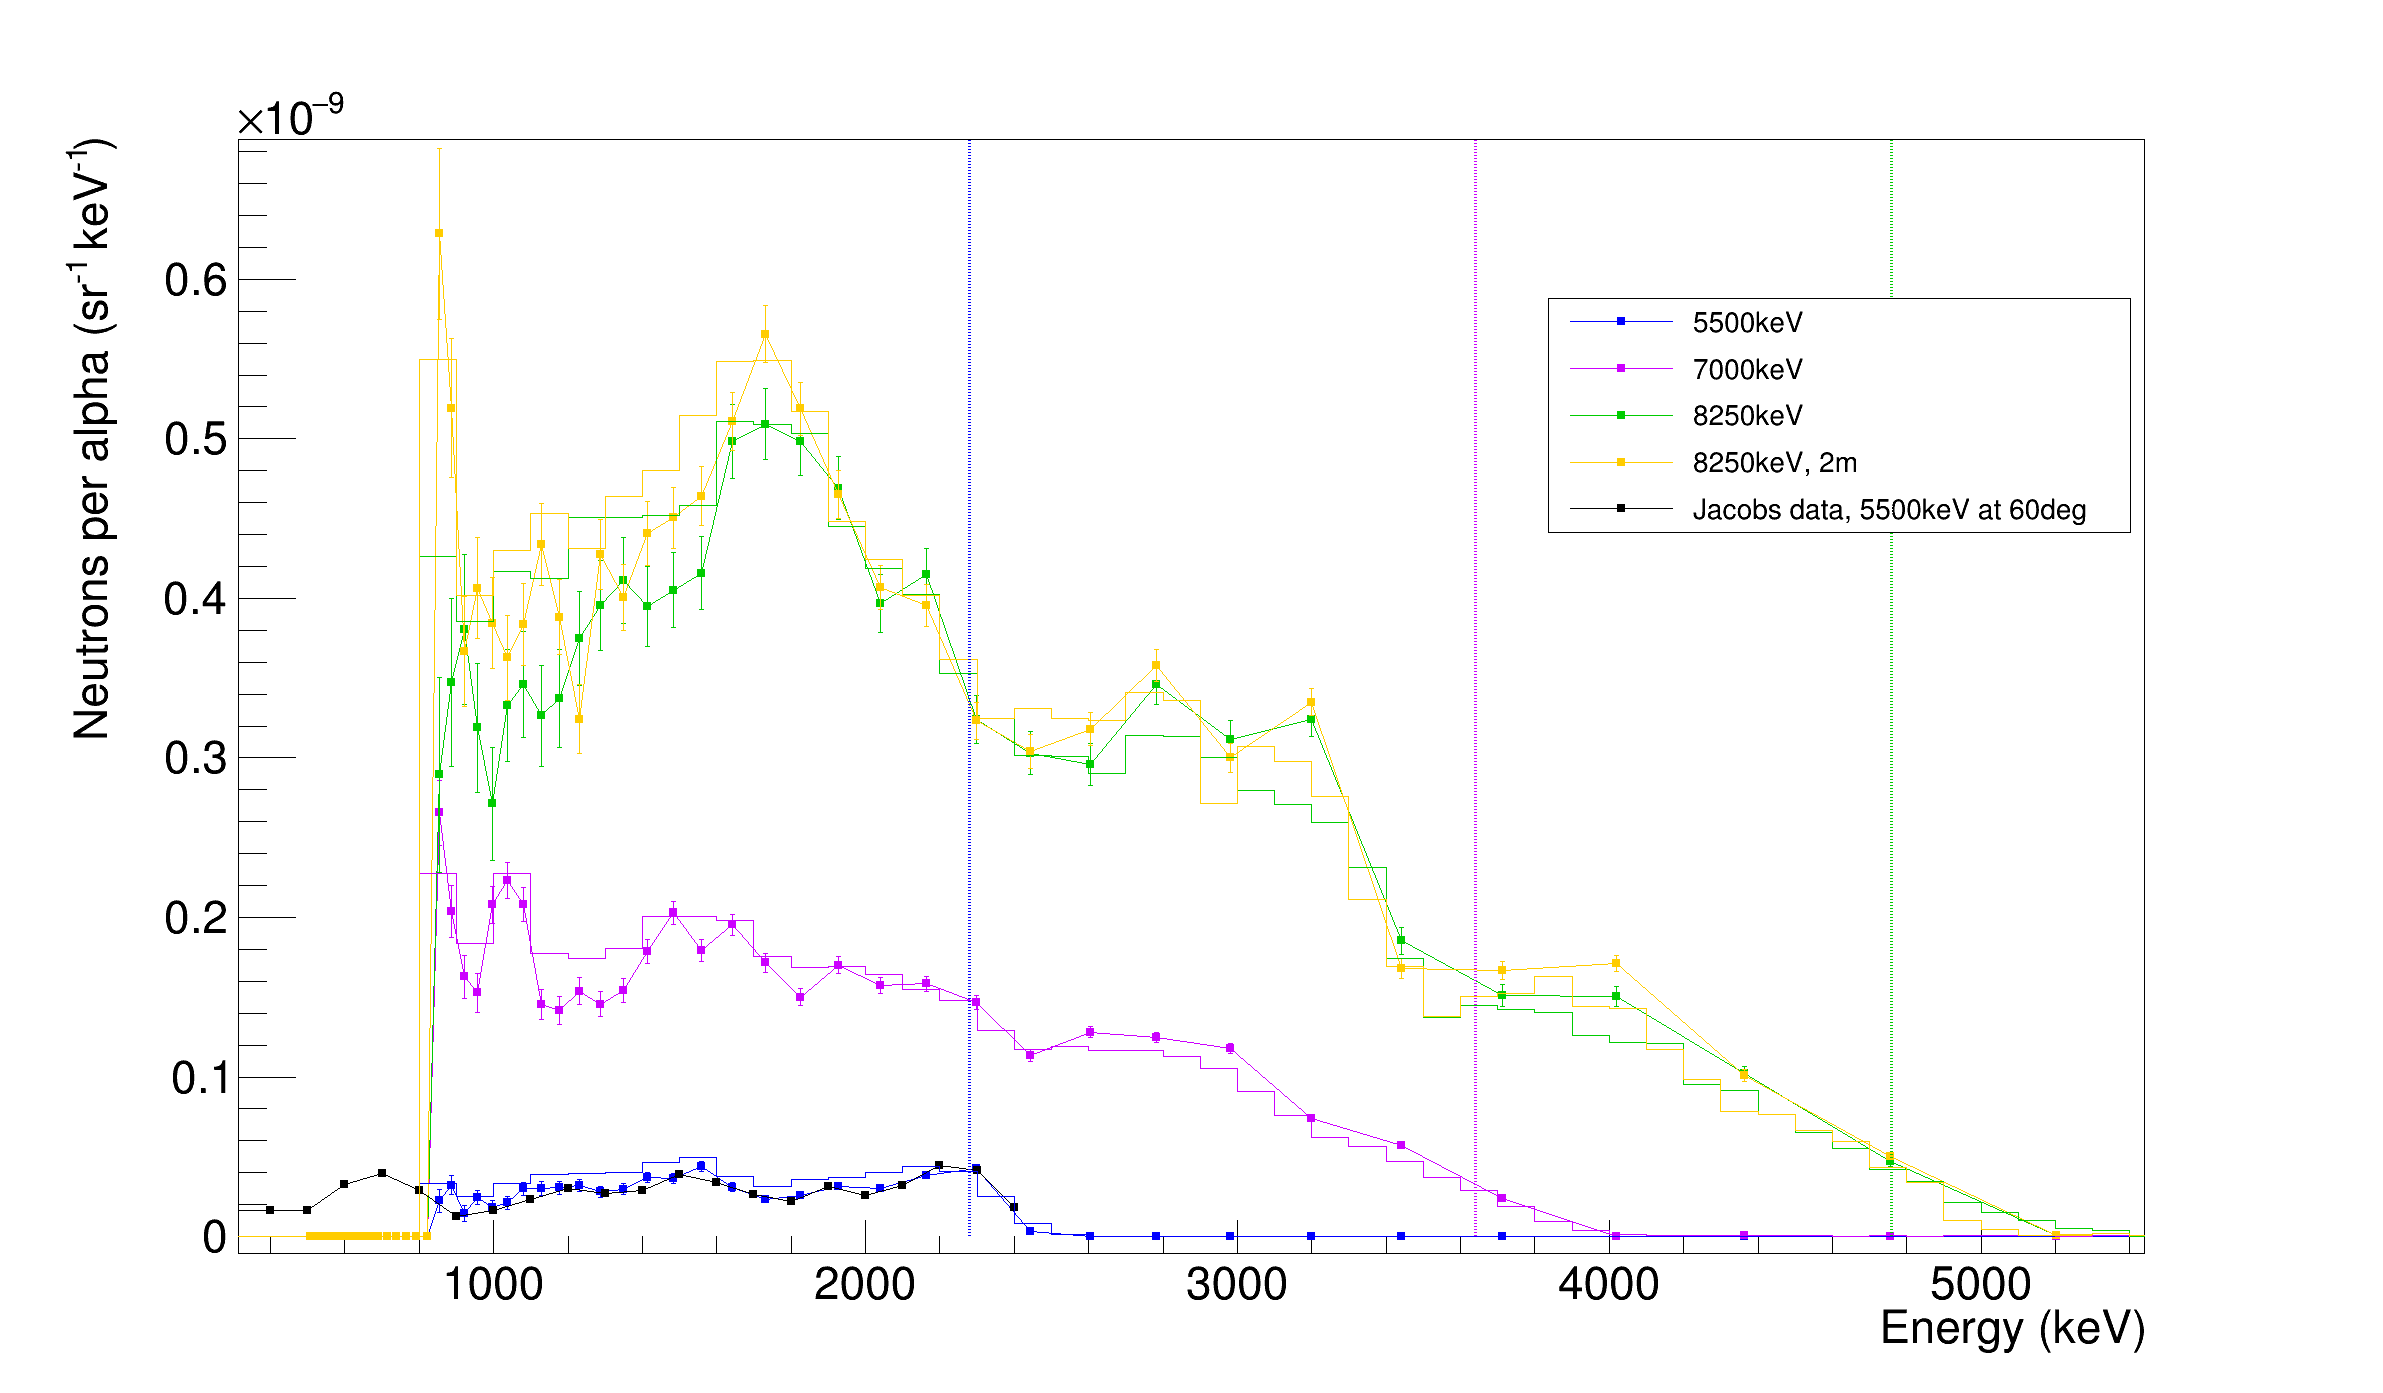
\includegraphics[width=0.80\textwidth]{pulsed_results.png}
	\caption{EXFOR data (black) and results for all of the time-of-flight measurements.
	The histograms are the simple method, the connected squares are the results of deconvolution, and the vertical dotted lines are the theoretical maximum neutron energies.}
	\label{pulsed_results}
\end{figure}

\chapter{Conclusions}
·We have managed to measure \an reaction yield in \Aliso with X uncertainty (given different detectors, days or months) and X agreement with previous measurements.\\
·We have managed to measure the corresponding neutron energy spectra with X uncertainty/resolution and X agreement with previous measurements.\\
·Improvements.\\

\begin{thebibliography}{5}
	\bibitem{neutron_in_an}Neutron production in \an reactions, \url{https://doi.org/10.1016/j.nima.2020.164095}
	\bibitem{}\url{https://doi.org/10.1016/j.nima.2009.04.032}
	\bibitem{}\url{https://doi.org/10.1016/j.nima.2017.09.007}
	\bibitem{nucleardatasheets}Nuclear Data Sheets 111, 2331 (2010), M. Shamsuzzoha Basunia.
\end{thebibliography}

\end{document}
